\def\nevergradnewbranch{OptimSuite}
\def\ngoptq{ABBO}


\chapter{Black-Box Optimization Revisited: Improving Algorithm Selection Wizards through Massive Benchmarking}
%{Towards Dynamic Algorithm Selection for Numerical\\ Black-Box Optimization: Investigating BBOB as a Use Case}
% \subtitle{Subtitle}
\label{paper:benchmark}

% \LetLtxMacro\latexincludegraphics\includegraphics
% \renewcommand{\includegraphics}[2][]{%
%   {\latexincludegraphics[#1]{#2}}}

Existing studies in black-box optimization suffer from low generalizability, caused by a typically selective choice of problem instances used for training and testing of different optimization algorithms. Among other issues, this practice promotes overfitting and poor-performing user guidelines. We address this shortcoming by introducing in this work a general-purpose algorithm selection wizard that was designed and tested on a previously unseen breadth of black-box optimization problems, ranging from academic benchmarks to real-world applications, from discrete over numerical to mixed-integer problems, from small to very large-scale problems, from noisy over dynamic to static problems, etc. Not only did we use the already very extensive benchmark environment available in Nevergrad, but we also extended it significantly by adding a number of additional benchmark suites, including Pyomo, Photonics, LSGO, and MuJoCo. Our wizard achieves competitive performance on all benchmark suites. It significantly outperforms previous state-of-the-art algorithms on some of the suites, including YABBOB and LSGO. Its excellent performance is obtained without any task-specific parametrization. 

The algorithm selection wizard, all of its base solvers, as well as the benchmark suites are available for reproducible research in the open-source Nevergrad platform.

% Note that keywords are not normally used for peerreview papers.



\section{Introduction: State of the Art}\label{sota}
Many real-world optimization challenges are effectively black-box problems; i.e., the main source of information when solving them is the evaluation of solution candidates. {These evaluations} often {require} simulations or even physical experiments. {Black-box optimization methods are thus widely applied in practice, with a particularly growing impact in} machine learning~\cite{salimans2016improved,lamcts}, to the point that they are considered a key research area of artificial intelligence. Black-box optimization algorithms are typically easy to implement and easy to adjust to different problem types. To achieve peak performance, however, proper algorithm selection and configuration are key, since black-box optimization algorithms have complementary strengths and weaknesses~\cite{rice1976,kerschke2018survey}. But while {automated} algorithm selection has become standard in SAT solving~\cite{satzilla} and AI planning~\cite{AIplanning}, {a manual selection and configuration of the algorithms---often entirely based on users previous experience and not necessarily on broader performance data---is still predominant in the broader black-box optimization context.}
% it is not yet widely used in the broader black-box optimization context.%, mostly due to an overspecialization of existing training sets.
{To reduce the bias inherent to such manual choices, and to support the automation of algorithm selection and configuration, sound comparisons of the different black-box optimization approaches are needed.}  
% Black-box optimization benchmarking aims to assist users and automated algorithm design tools in the challenging task of choosing the right algorithm and the right parameters for a given problem.
% \antoine{The real time aspect (ie chaining) is not evoked here, is it ok? }
% the overspecialization is explained a bit more in Generalization (under Desirable Features)
%in this challenging task. % I think the "overspecialization" is actually explained below: 
Existing benchmarking suites, however, are rather selective in the problems they cover. This leads to specialized algorithm frameworks whose performance suffer from poor generalizability. 
{We address this flaw in black-box optimization by presenting a high-performing algorithm selection wizard, \ngoptq{} ({Automated Black-Box Optimization}). \ngoptq{} uses very basic information about the problem and the available computational resources to select one or several algorithms, which are run for the allocated budget of function evaluations. The wizard was developed within the Nevergrad platform~\cite{nevergrad}, which we have significantly extended for this work to obtain an even broader set of benchmark problems.}

%\url{https://dl.fbaipublicfiles.com/nevergrad/allxps/list.html}. 
% For ICLR reviewers, all code  is available, thanks to github-anonymizer, at~\cite{source}. %\url{https://anonymous.4open.science/r/5118cc2c-e2b0-475f-ba8d-3a2971a93acd/}.

In summary, our key contributions are as follows: 
\underline{\textbf{(1) Algorithm Selection Wizard \ngoptq{}:}} Our algorithm selection technique, \ngoptq{} can be seen as an extension of the Shiwa wizard presented in~\cite{versatile}. 
The wizard takes as input information on the \emph{problem} (the dimension of the search domain, the type and range of each variable, and their order), the \emph{presence of noise} in the evaluation (but not its intensity), and the \emph{computational resources} that are available to solve the problem (the budget and the degree of parallelism, i.e., number of solution candidates that can be evaluated simultaneously). Based on this input, the wizard outputs one or several algorithms that it suggests to execute on the given problem. 
\ngoptq{} uses three types of selection techniques: 
\emph{passive algorithm selection} (choosing an algorithm as a function of a priori available features~\cite{versatile}), 
\emph{active algorithm selection} (a bet-and-run strategy which runs several algorithms for some time and stops all but the strongest {after a predefined number of evaluations}~\cite{mersmann2011,pitzer2012,FischettiM14,malan2013,munoz2015_as,cauwet2016algorithm,kerschke2018survey}), % Note that active algorithm selection is sometimes referred to as ``bet-and-run strategy''~\cite{FischettiM14}, 
and \emph{chaining} (running several algorithms in turn, in an a priori defined order~\cite{chaining}). 

Our wizard selects from and combines a very large number of base algorithms, among them algorithms suggested in~\cite{scipy,cma,de,powell,cobyla,versatile,beyerhellwignoise,artelyssqp2,fastga,adaptivecarola}. We compare the performance of \ngoptq{} to all these algorithms, as well as to its predecessor Shiwa, and to all other algorithms available in Nevergrad. 

\underline{\textbf{(2) Benchmark Collection:}} By integrating a number of additional benchmark suites into the Nevergrad platform, we obtain a huge benchmark collection that covers a previously unseen breadth of black-box optimization problems, ranging from academic benchmarks to real-world applications, from discrete over numerical to mixed-integer problems, from small to very large-scale problems, from noisy over dynamic to static problems, etc. 
% Details about this collection are available in Sec.~\ref{bench}. 
%combines several contributions that recently led to improved reliability and generalizability of black-box optimization benchmarking, 
% among others, LSGO~\cite{lsgo}, YABBOB~\cite{bbob,versatile}, Pyomo~\cite{pyomo}, MLDA~\cite{mlda}, and MuJoCo~\cite{mujoco,ars,lgrs}. {A more detailed summary can be found in Sec.~\ref{bench}).} 

{
\textbf{Structure of the Paper:} We motivate in Sec.~\ref{bench} why we have chosen to develop \ngoptq{} within the Nevergrad benchmarking environment and how we have extended it. Sec.~\ref{ngopt} summarizes \ngoptq{} and discusses differences to previous versions. Experimental results can be found in Sec.~\ref{xpr}. Sec.~\ref{sec:conclusions} concludes our paper with an outlook to future work.} 

{\textbf{Availability of Data and Code:} Our algorithm selection wizard \ngoptq{}, its base solvers, and the benchmark collection have all been merged to the \textbf{main Nevergrad master}, where they are available for reproducible, open-source research. Nevergrad periodically reruns all algorithms and makes all data available on the \textbf{public dashboard}~\cite{dash}. Note that ABBO is called \textbf{NGOpt8} within the Nevergrad environment, to allow for better version control in the latter: NGOpt is the name of the latest version of the optimization wizard, the current version (July 2021) is NGOpt14. Since Nevergrad is developing at fast pace, we have saved a \textbf{frozen version of its code base}. Together with the \textbf{performance data} used for this paper and the \textbf{videos} illustrating the performance of the policies learned for MuJoCo, this code is available on zenodo~\cite{zenodo}. }%change


\def\papa{p{0.3\textwidth}}
\def\pupu{p{0.1\textwidth}}
\def\popo{p{0.055\textwidth}}

% \begin{figure}[t]
%     \includegraphics[width=.55\textwidth]{benchmark/xp_yabbob.png}
%       \includegraphics[width=.4\textwidth]{benchmark/fa_yabbob.png}\\
       
%         %\twocaptions[Avg. norm. loss]{Heatmap}\\
% %    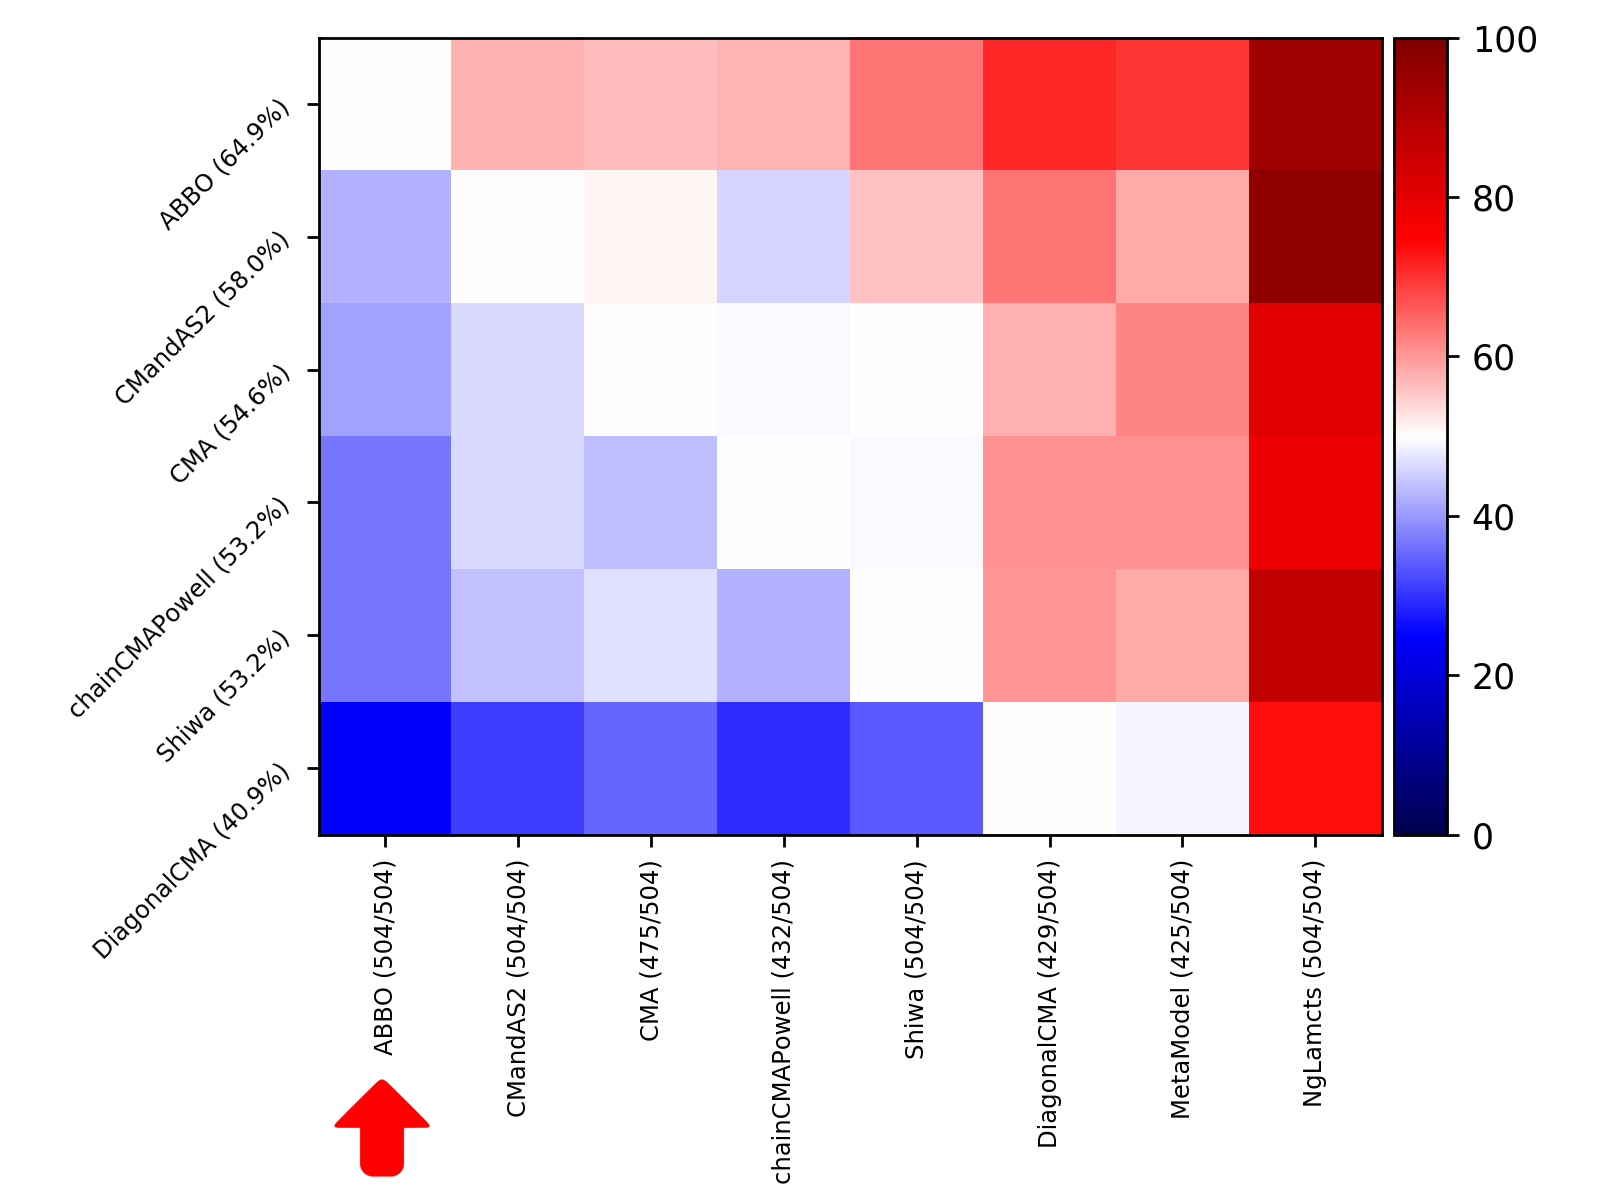
\includegraphics[width=.4\textwidth]{benchmark/fa_yabigbbob.png}
% %        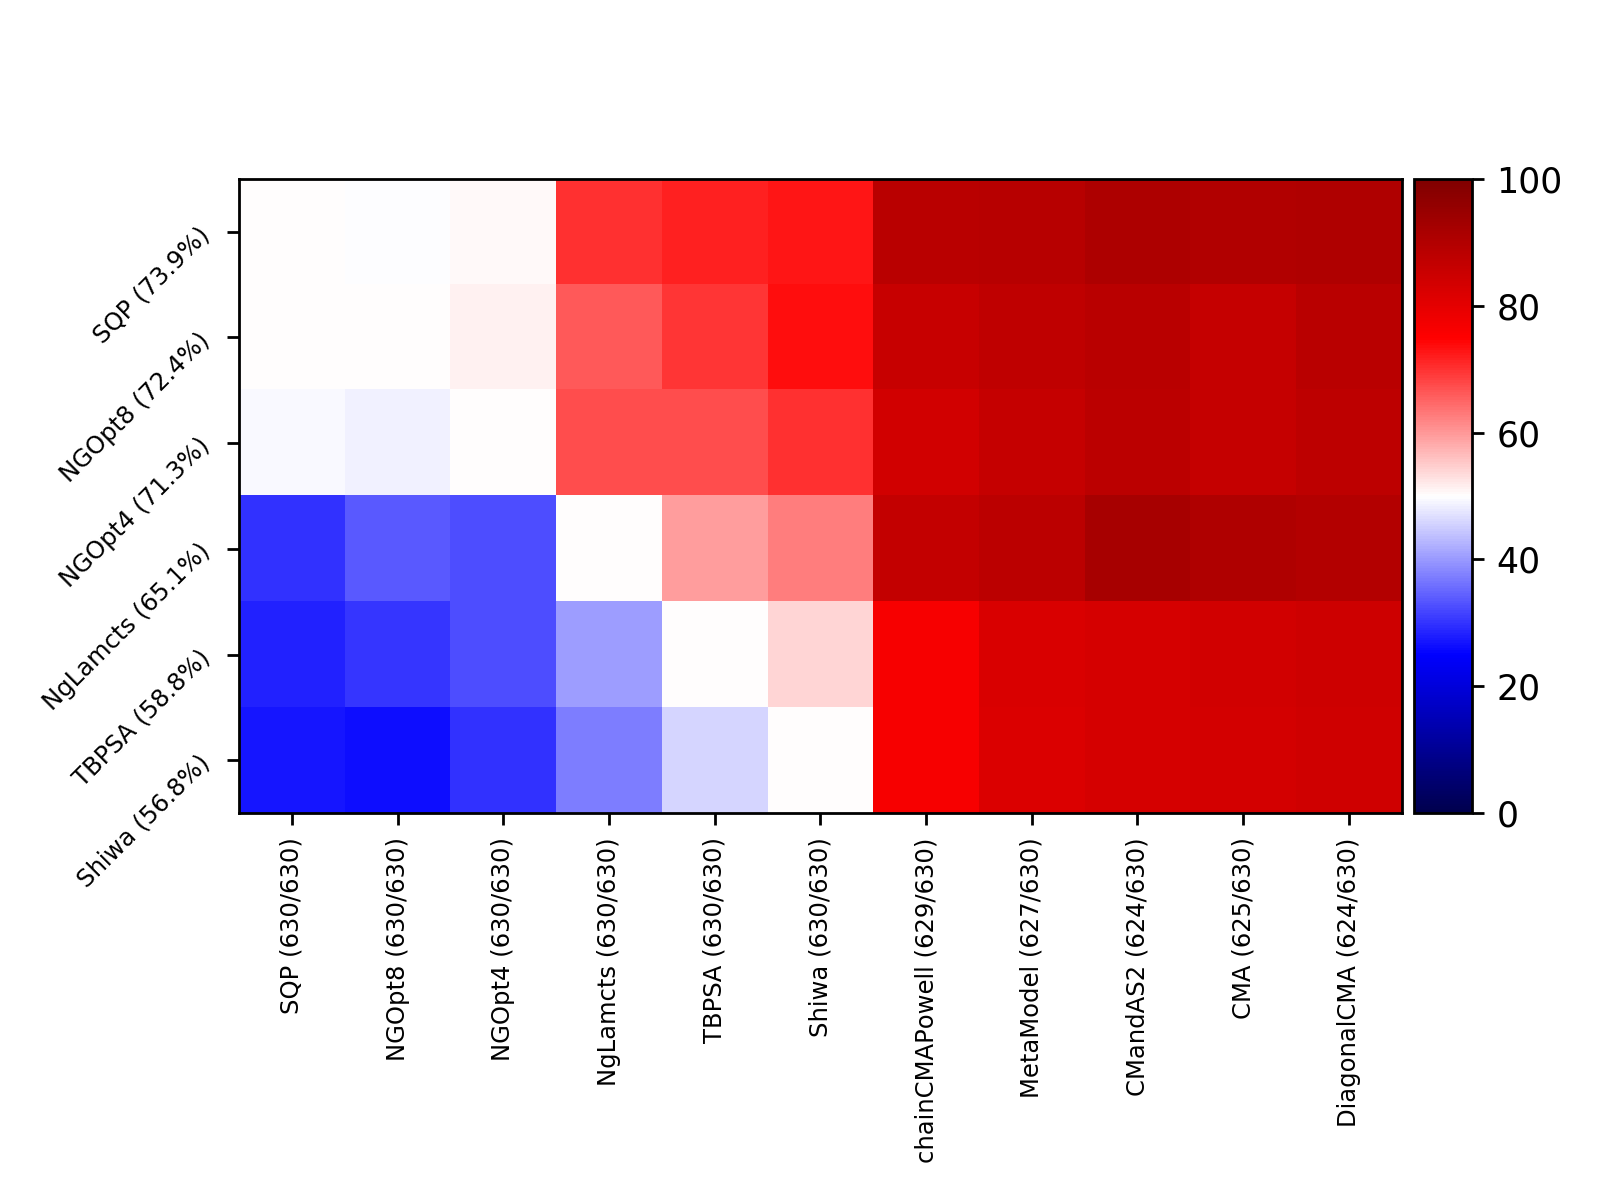
\includegraphics[width=.4\textwidth]{benchmark/fa_yanoisybbob.png}
% %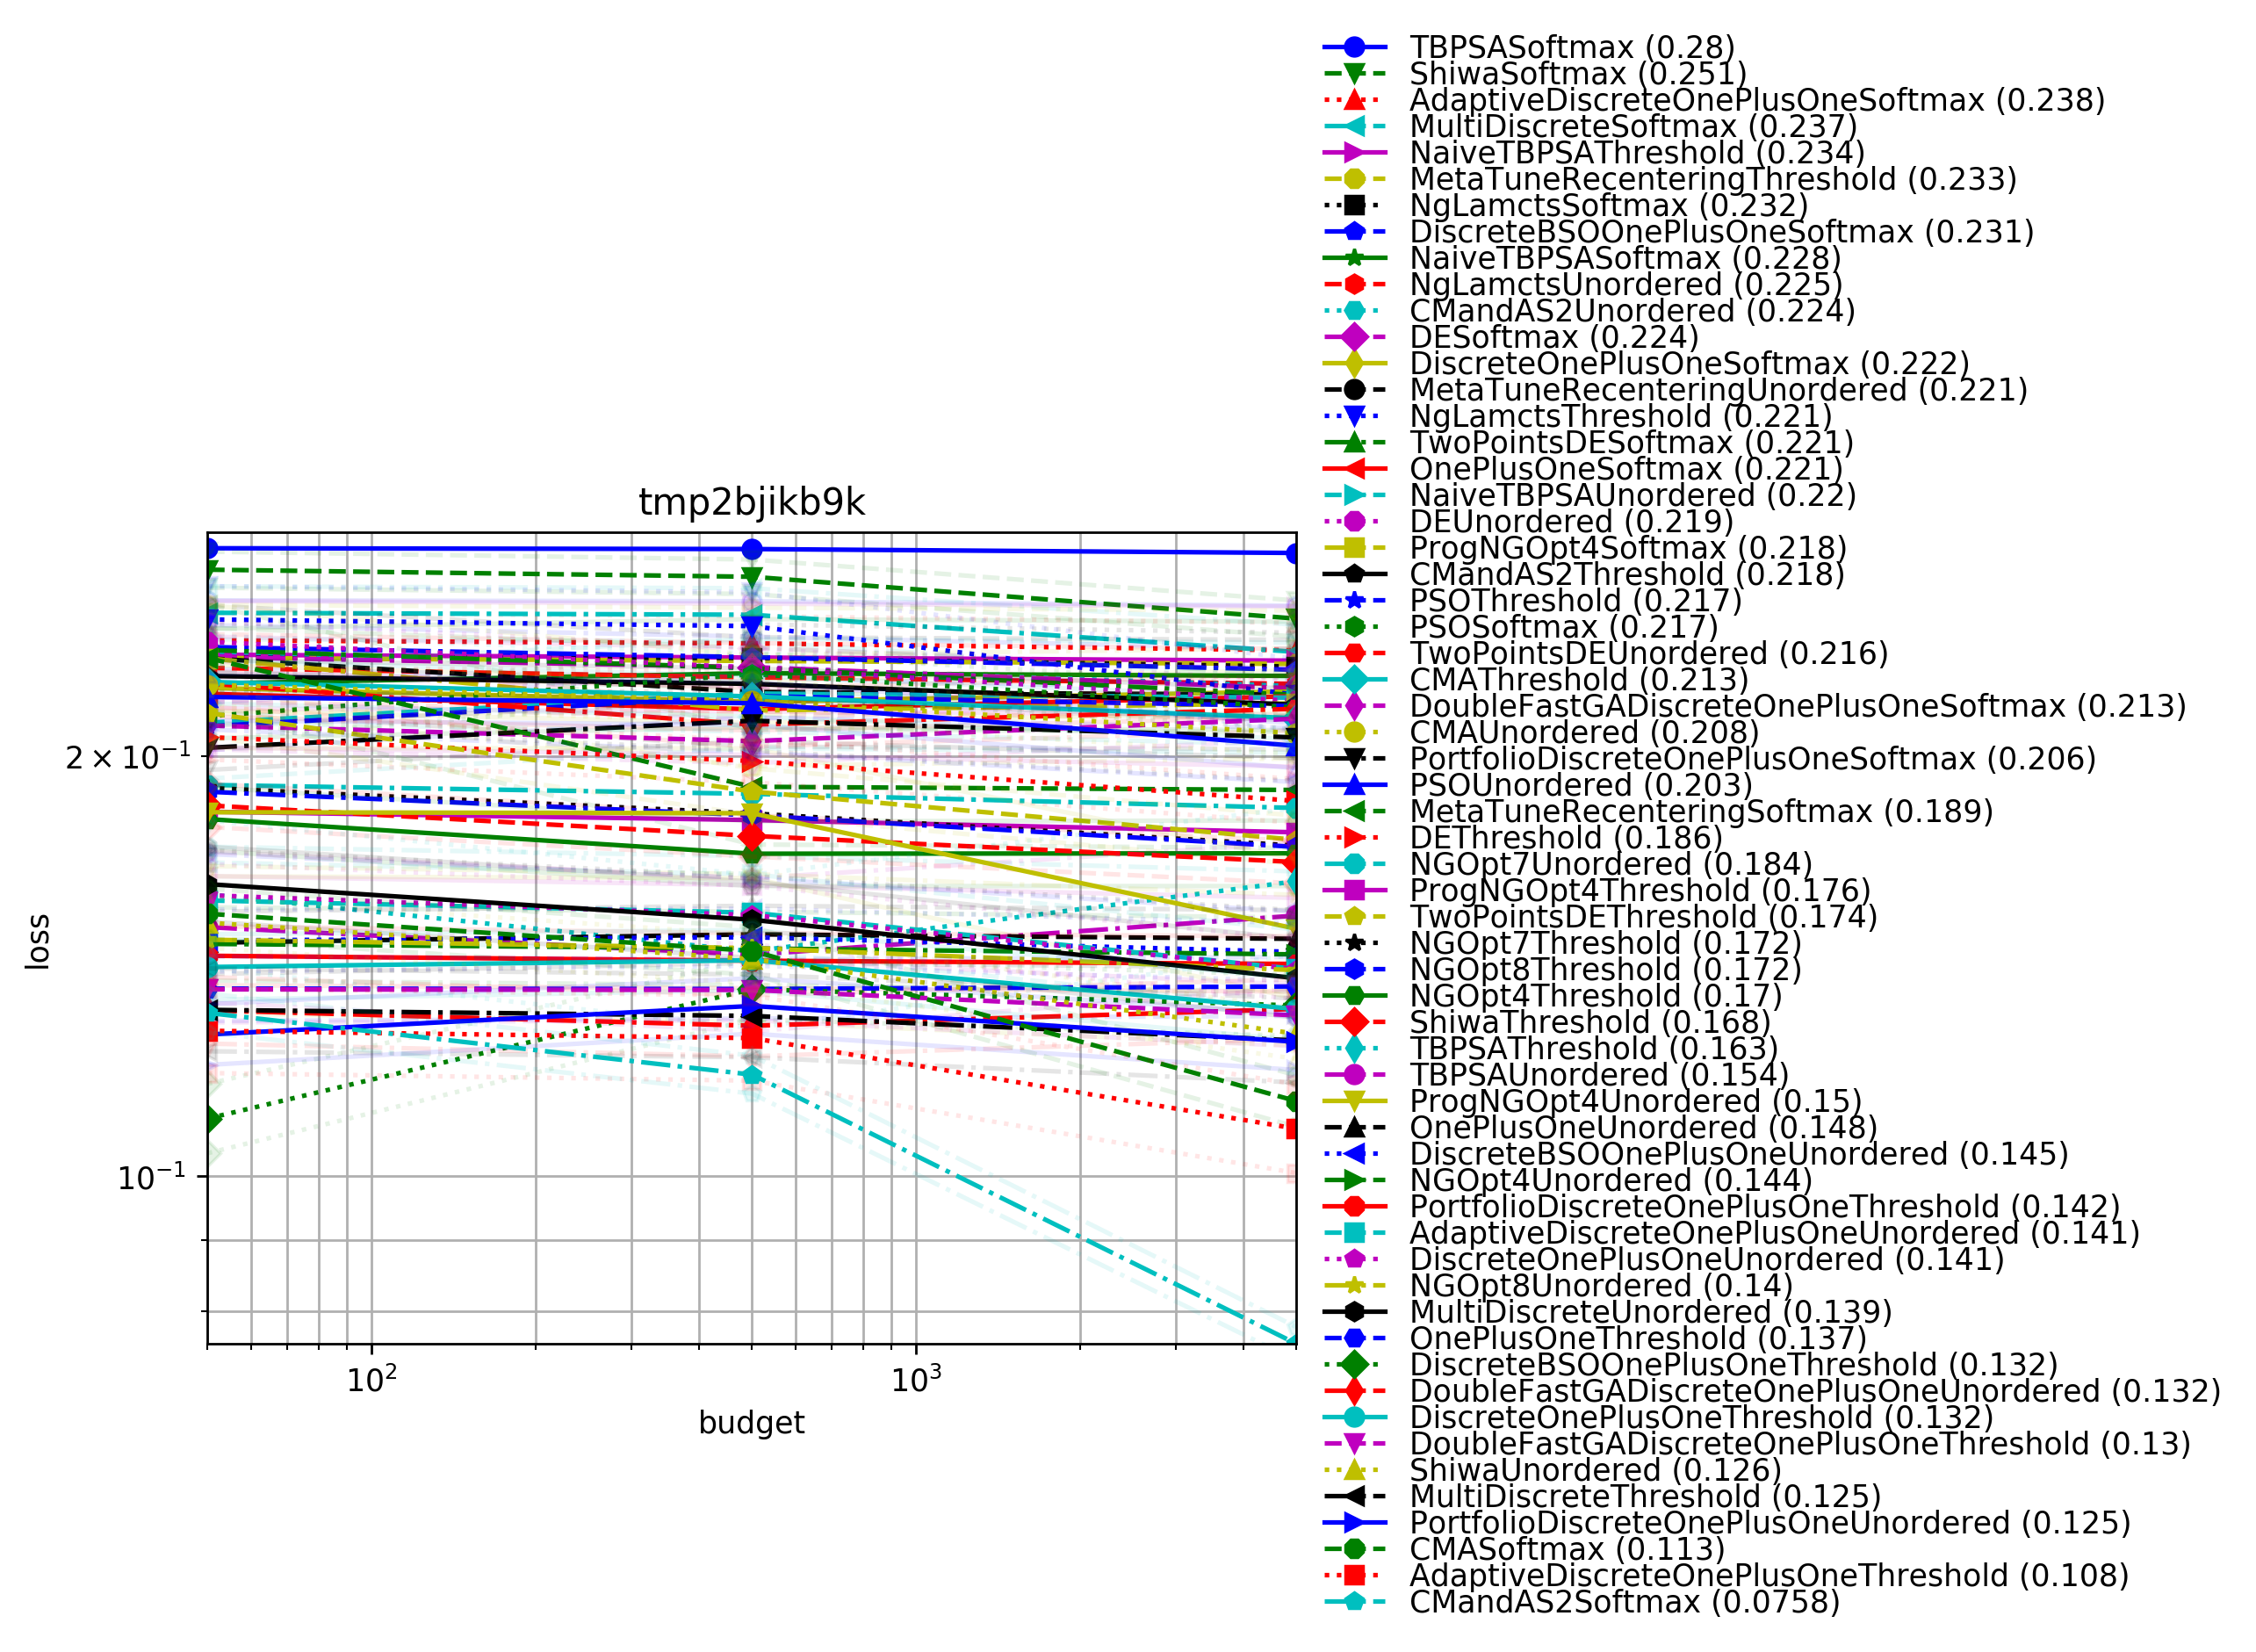
\includegraphics[width=.4\textwidth]{benchmark/xp_instrum_discrete.png}
% %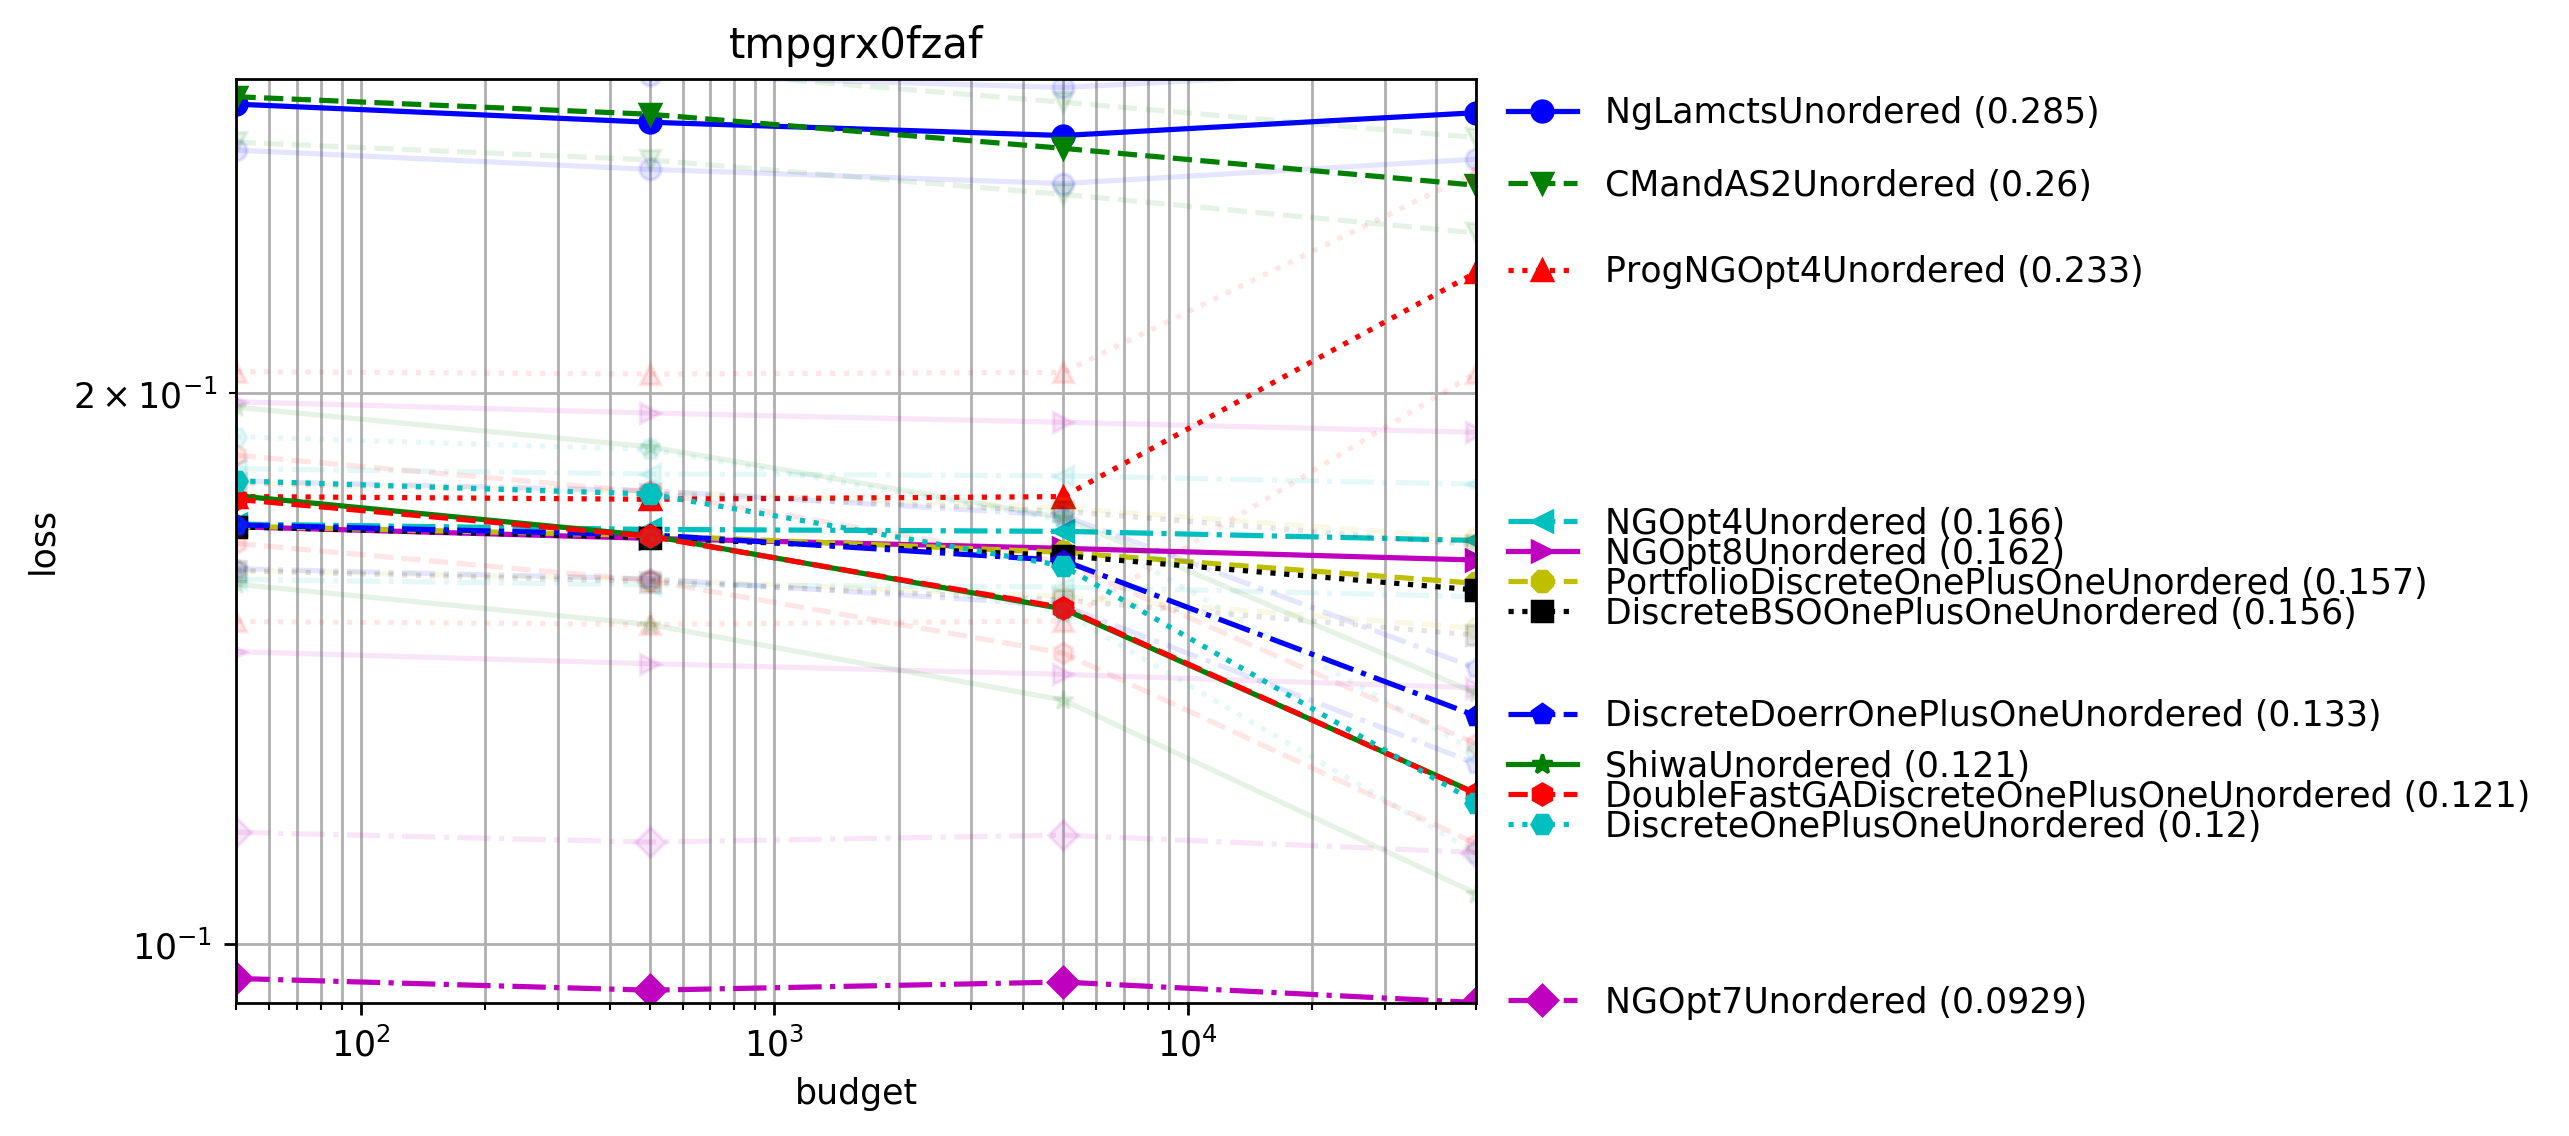
\includegraphics[width=.4\textwidth]{benchmark/xp_sequential_instrum_discrete.png}\\
% %%\twocaptions[InstrumDiscrete]{SequentialInstrumDiscrete}
% 	\caption{Average norm loss and heatmap for YABBOB. Additional plots for High-dimensional (HD), NoisyHD and Large budgets are available in Appendix~\ref{addfig}. Other variants include parallel, differences of budgets and combinations of those variants, with excellent results for \ngoptq{} (see Nevergrad's dashboard~\url{https://dl.fbaipublicfiles.com/nevergrad/allxps/list.html}, publicly visible with anonymized entries, for the part of our code which is already merged).}
%     \label{bbobfig}
% \end{figure}
% \begin{figure}[t]
%     \centering
%     \includegraphics[trim={0 0 0 150},clip,width=.485\textwidth]{benchmark/xp_alldes.png}
%     \includegraphics[trim={0 0 0 45},clip,width=.485\textwidth]{benchmark/xp_hdbo4d.png}\\
% 	%\twocaptions[AllDEs ($d\in\{5, 20,100\}$.)]{HDBO ($d\in\{20,2\,000\}$)}
% %\twocaptions[Cigar, Hm, Ellipsoid, Sphere.]{Cigar, Hm, Ellipsoid, Sphere.}
% %    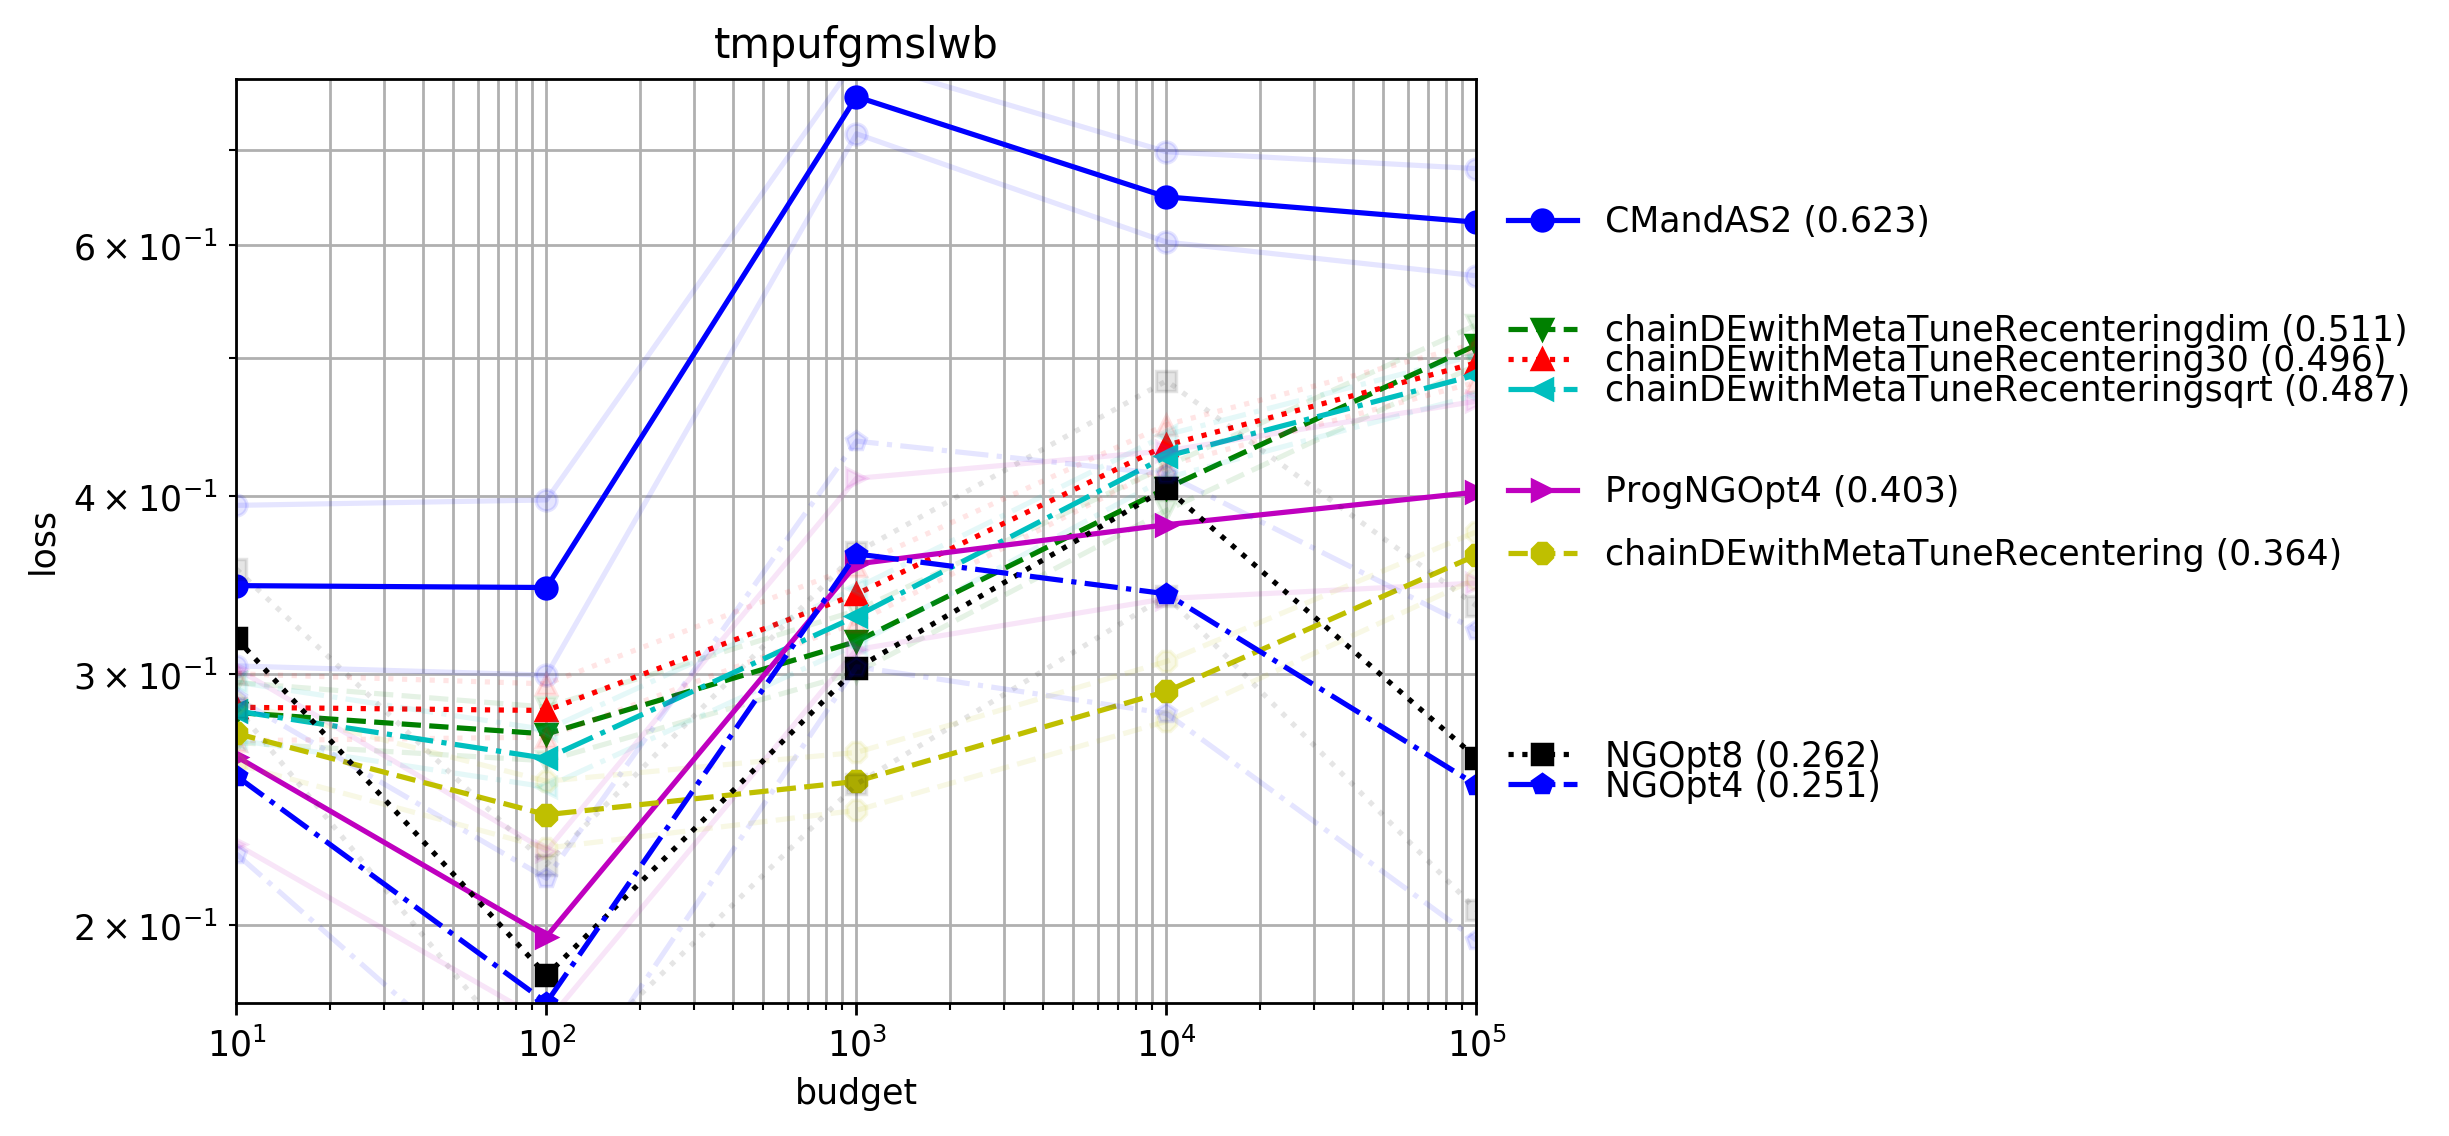
\includegraphics[width=.4\textwidth]{benchmark/xp_paraalldes.png}\\   
% %    %\twocaptions[AllDEs]{Para-AllDEs}
% %    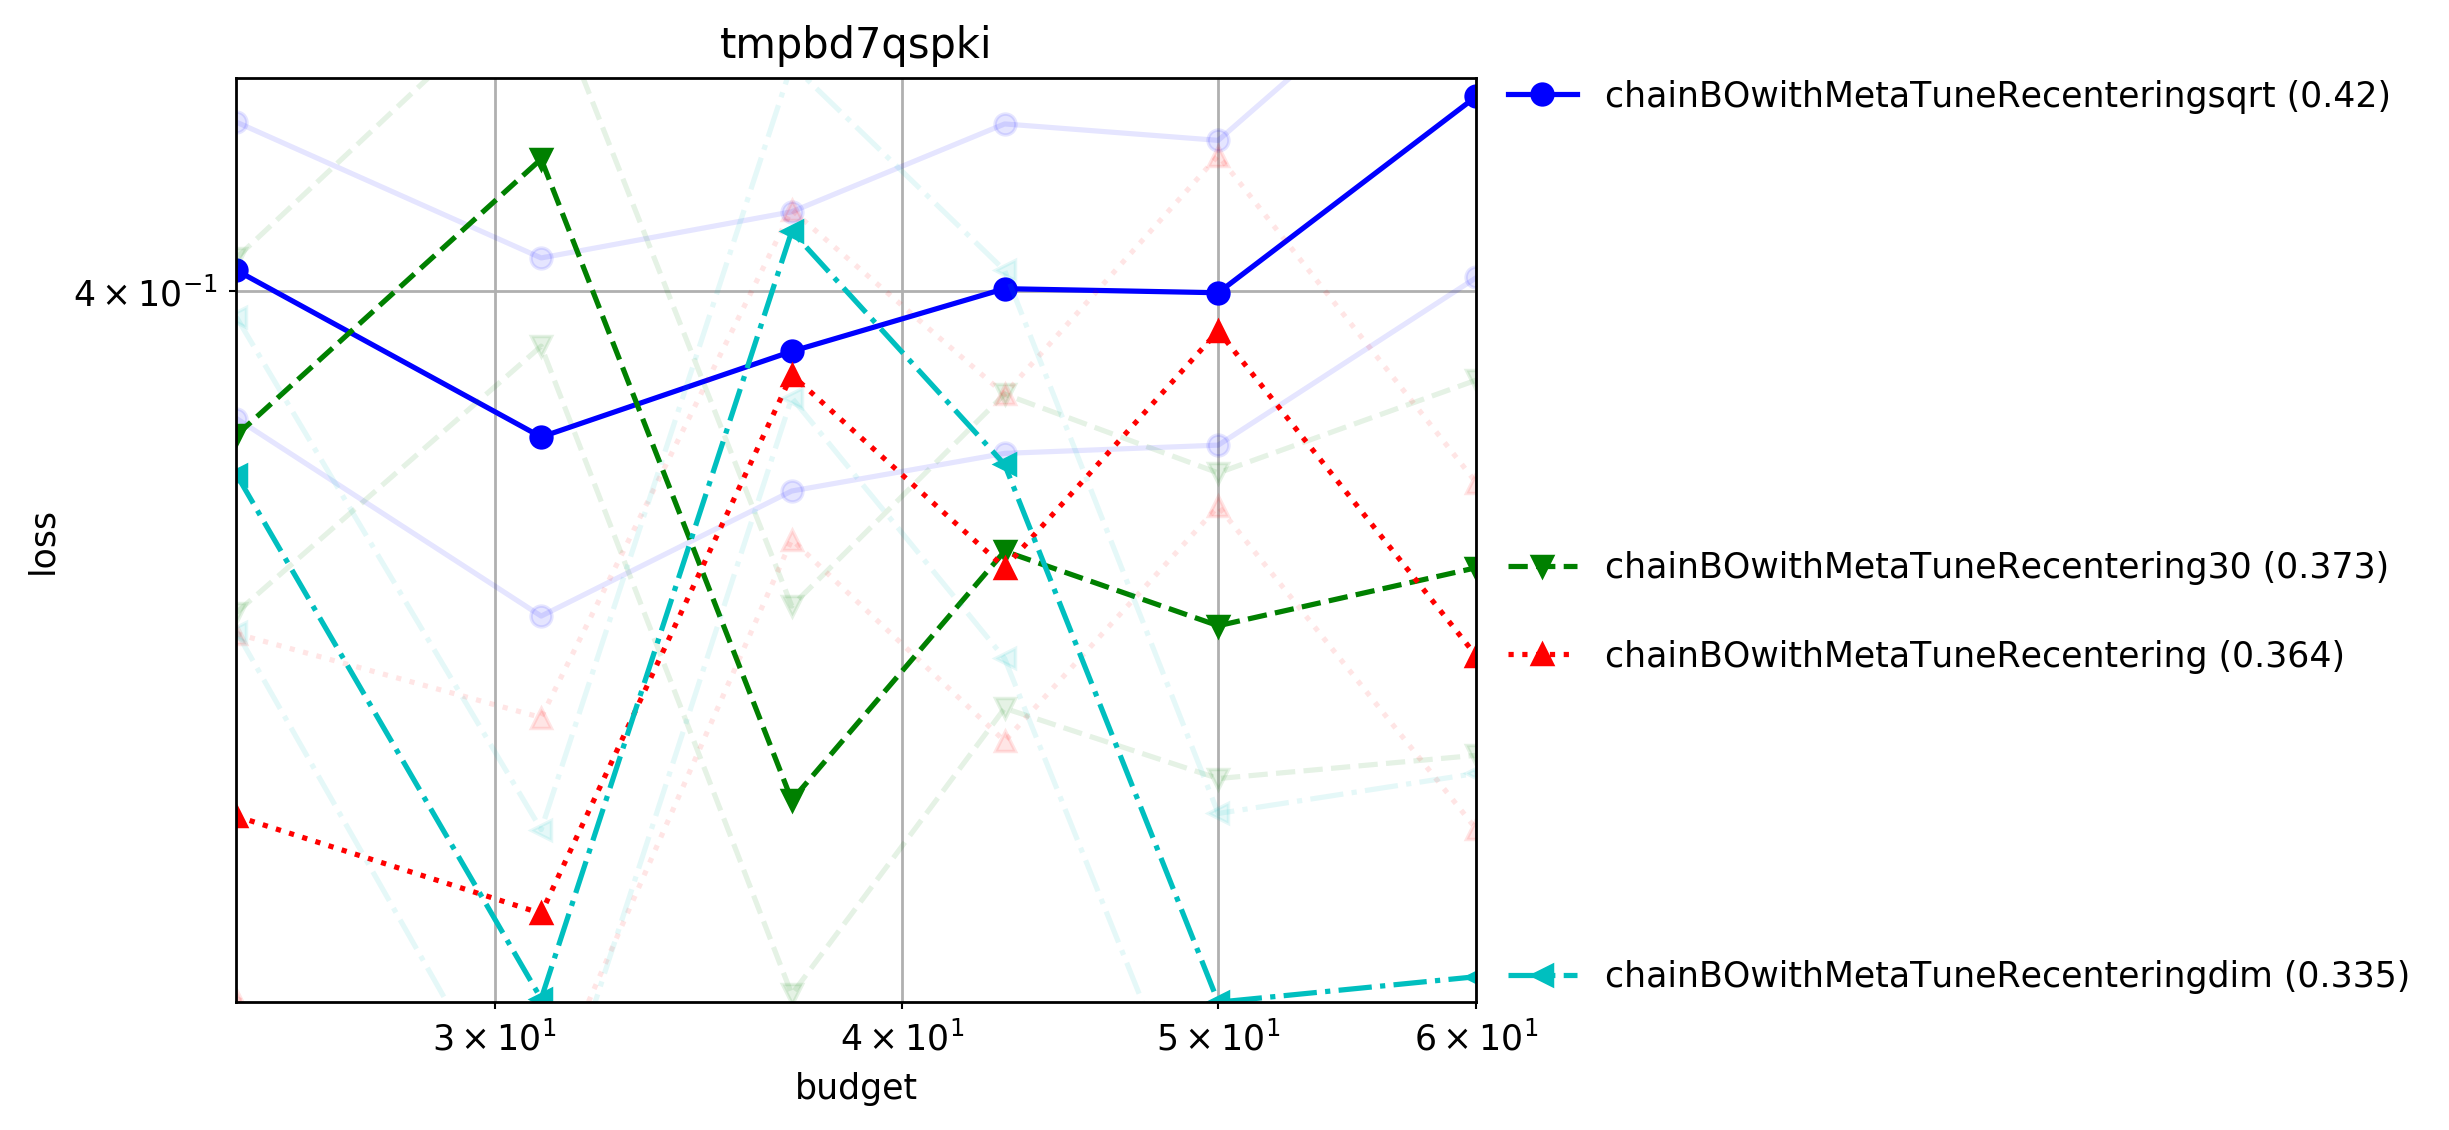
\includegraphics[width=.4\textwidth]{benchmark/xp_parahdbo4d.png}\\
% %    %\twocaptions[HDBO]{Para-HDBO}
%     \caption{\ngoptq{} vs specific families of optimization algorithms (DE, and BO in the high-dimensional case). Not all run algorithms are mentioned, for short. {Bayesian optimization {(Nevergrad uses \cite{BOpython})}, often exploring boundaries first, is outperformed in high dimension}~\cite{lamcts}.}
%     \label{specif}
% \end{figure}
% \begin{figure}[t]
% \centering
% \includegraphics[trim={0 0 0 54},clip,width=.45\textwidth]{benchmark/xp_paramultimodal.png}%\includegraphics[width=.4\textwidth]{benchmark/fa_far_optimum_es.png}\\
% 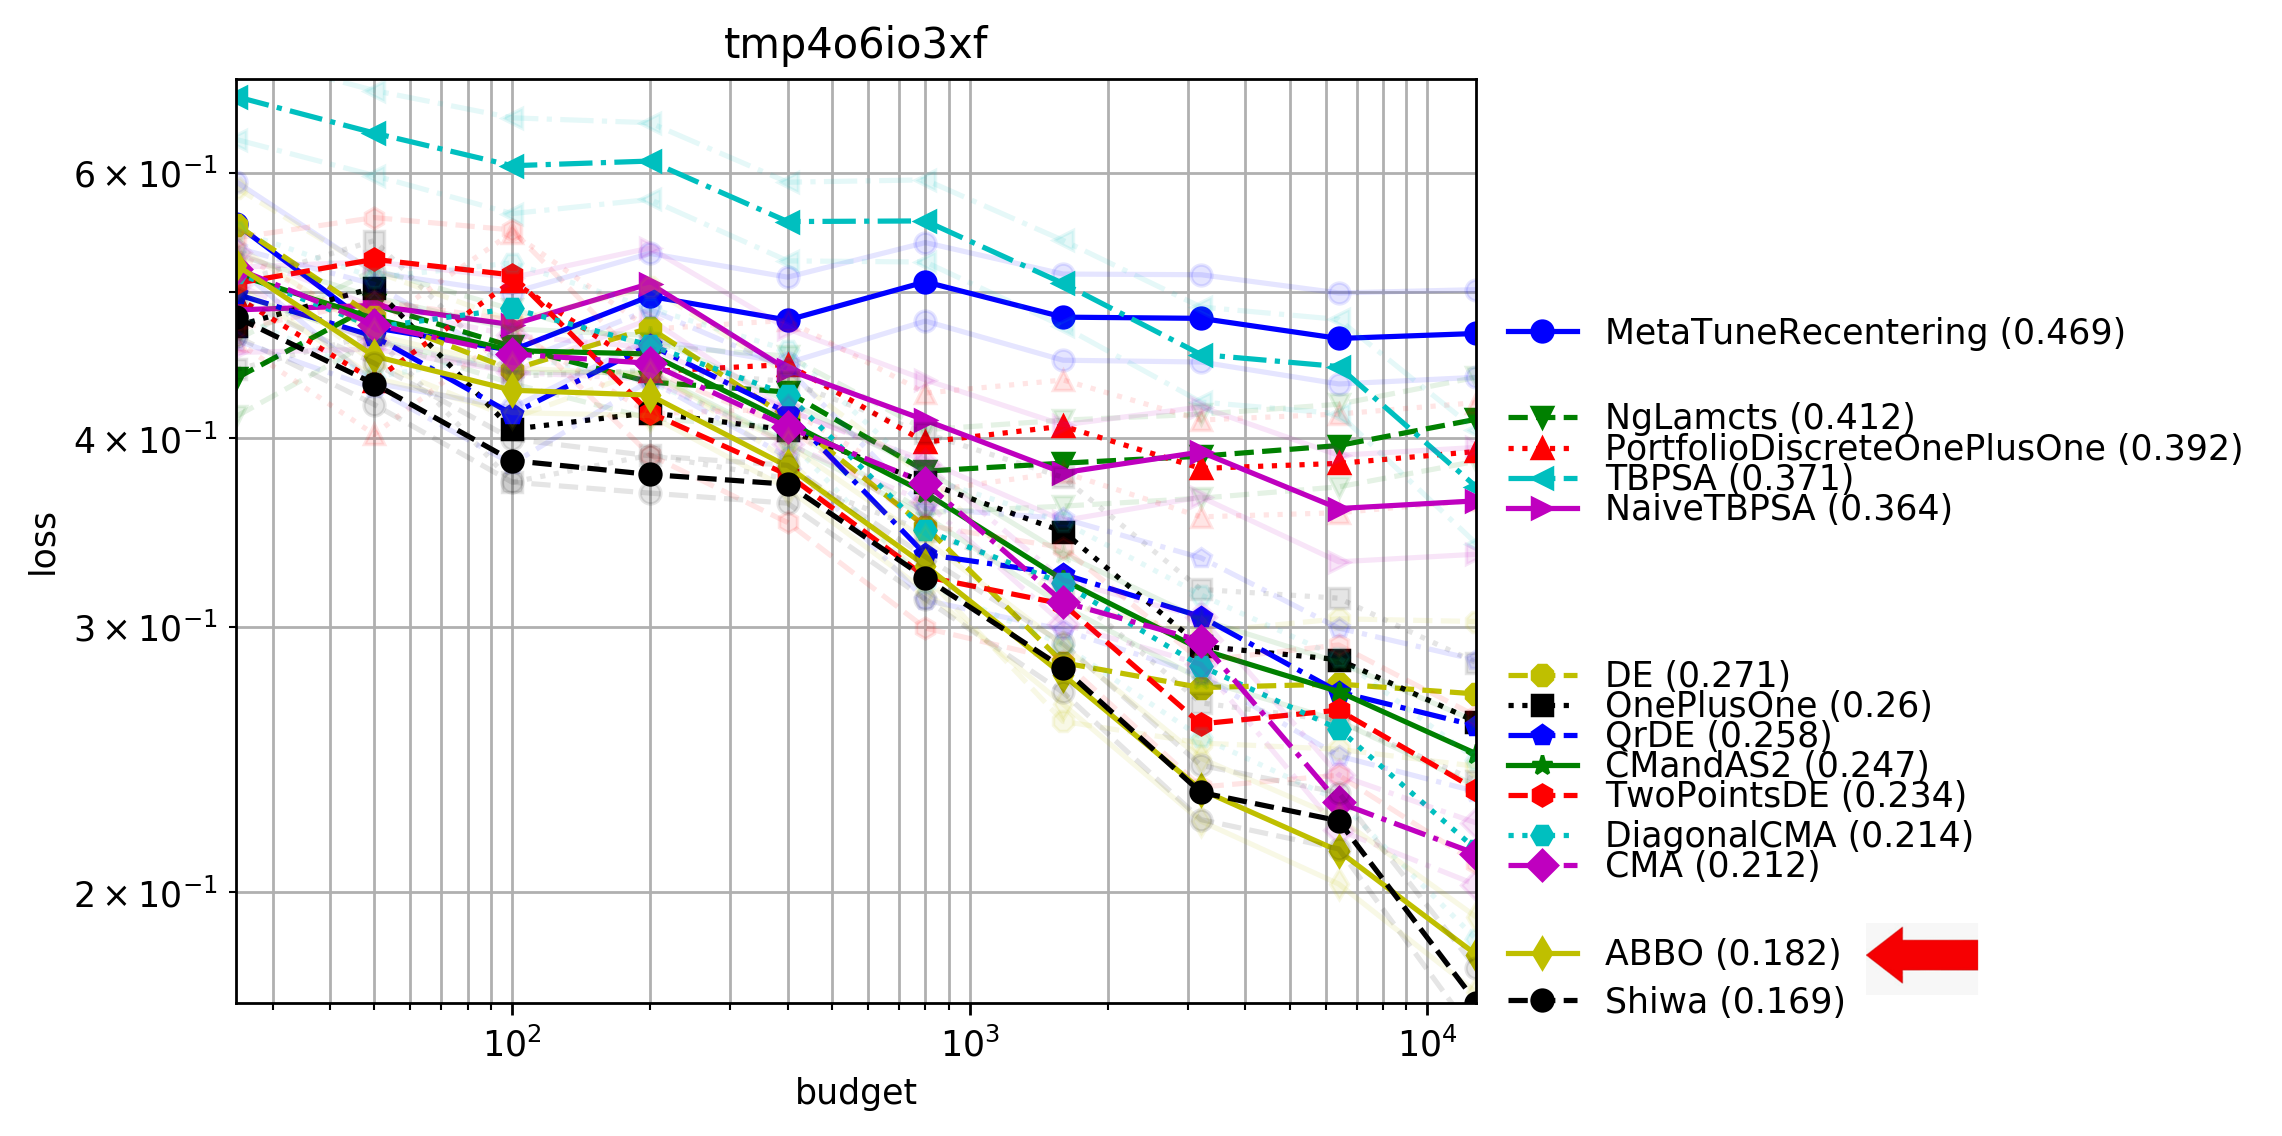
\includegraphics[trim={0 0 0 21},clip,width=.49\textwidth]{benchmark/xp_realworld.png}%\includegraphics[width=.4\textwidth]{benchmark/fa_realworld.png}\\ 
% 	\caption{Left: experiments for the parallel multimodal setting PARAMULTIMODAL. Budget up to 1\,00000, parallelism 1\,000, Ackley+Rosenbrock+DeceptiveMultimodal+Griewank+Lunacek+Hm. Right: Realworld benchmark from Nevergrad: games, Sammon mappings, clustering, small traveling salesman instance, small power systems.}\label{figrw}
% \end{figure}



\begin{table*}[ht]
\centering
	\caption{\label{overview} Properties of selected benchmark collections (details in the main text). ``+'' means that the feature is present, ``-'' that the feature is missing, and ``NA'' means that it is not applicable.}
\scriptsize
\begin{tabular}{|c|c|c|c|c|c|}
	\hline
		Testbed & BBOB & MuJoCo& LSGO & BBComp& Nevergrad \\
	\hline
	\hline
		Large scale     & - & NA & + & -  & + \\
		Translations    & + & NA& +  & + & + \\
		Symmetrizations / rotations & + & NA& +  &  -& + \\
		One-line reproducibility& - & - & -  & -& + \\
		Periodically automated dashboard & NA & NA& NA & NA & + \\
		Complex or real-world & - & + & -  & +& + \\
		%Multimodal & + & + & + & + & + \\
		Available open source and no licensing issues & +  & - &  + &  + & + \\
		Ask/tell/recommend framework & - & NA& +  & + & + \\
% 		Far-optimum & + & NA & - & - & + \\
		Human excluded / client-server & -& -& -& + &- \\
		%Included in \nevergradnewbranch & + & + & + & + & + \\
	\hline
\end{tabular}
\end{table*}


\section{Sound Black-Box Optimization Benchmarking}\label{bench}

{We discuss in this section which features we consider desirable for sound benchmarking, and how different suites address these. This discussion motivates our decision to design and to evaluate \ngoptq{} within the Nevergrad environment~\cite{nevergrad}. Tab.~\ref{overview} summarizes how some of the common benchmarking environments address the properties discussed below.}

{\subsection{Desirable Properties for Sound Benchmarking}} %We now discuss the properties listed in Tab.~\ref{overview}.

{\textbf{Generalization:}} The most obvious issue in terms of generalization is the statistical one: we need sufficiently many experiments for conducting valid statistical tests and for evaluating the robustness of algorithms' performance. However, this is probably not the main issue. A biased benchmark, excluding large parts of the real world needs, leads to biased conclusions, no matter how many experiments we perform. Inspired by~\cite{cifargeneralize} in the case of image classification, {and similar to the spirit of cross-validation for supervised learning}, we use 
a much broader collection of benchmark problems for evaluating algorithms in an unbiased manner. 
Another subtle issue in terms of generalization is the case of instance-based choices of (hyper-)parameters: an experimenter modifying the algorithm or its parameters specifically for each instance can easily achieve considerable performance improvements. In this paper, we consider that only the following problem properties are known in advance (and can hence be used for algorithm selection and configuration): the dimension of the domain, the type and range of each variable, their order, the presence of noise (but not its intensity), the budget, and the degree of parallelism (i.e., number of solution candidates that can be evaluated simultaneously). 
To mitigate the common risk of over-tuning, we evaluate algorithms on a broad range of problems, from academic benchmark problems to real-world applications. Each algorithm runs on all benchmarks without any change or task-specific tuning. 

\textbf{Large scale:} Since practical problems can reach very large dimensions, we consider it desirable to include benchmark suites that comprise such problems. A ``+'' in Table~\ref{overview} indicates that the collection provides benchmark problems in dimension  $\geq1\,000$.   
%Whether or not the suite comprises problems in dimension  $\geq1\,000$.

\textbf{Translations:} {The search point} zero frequently plays a special role in optimization. For example, complexity penalization often ``pushes'' towards zero. 
 {Also, large values in a neural network lead to saturation~\cite{xavier}: then, we get a plateau and cannot learn from the samples.} %numbers far from zero are often more likely to lead to bang-bang solutions (and therefore extract zero signal, leading to a needle-in-the-haystack optimization situation), in particular with neural networks.
% In one-shot optimization,~\cite{icmldoe,ppsnrescaling} have shown how much focusing to the center is a good idea in particular in high-dimension.
% Our experiments in control {(in particular MuJoCo)} confirm that the variance of randomized searches is critical. This can explain some of the misleading results observed in some optimization papers (see Sec.~\ref{MuJoCo} for a discussion). 
In artificial experiments, several classical test functions have their optimum at $(0,\ldots,0)$. To avoid misleading conclusions, it is now a standard procedure, advocated in particular in~\cite{bbob}, to randomly translate the objective functions. %This is unfortunately not always applied. 
Concretely, we consider that there is translation when optima are randomly translated by a ${\mathcal N}(0,\sigma^2)$ shift. This property is mainly interesting for artificially created benchmarks, but is unfortunately not always applied.
% in unbounded continuous domains, a standard deviation $\sigma$ has to be provided, for example for sampling the first and second iterates of the optimization algorithm. G
% given a standard deviation $\sigma$, we consider that there is translation when optima are randomly translated by a ${\mathcal N}(0,\sigma^2)$ shift. Only interesting for artificial cases.


{\textbf{Symmetrizations / Rotations:}} Some optimization methods may perform well on separable objective functions but degrade significantly when optimizing non-separable functions. If the dimension of a separable objective function is $d$, these methods can reduce the objective function into $d$ one-dimensional optimization processes~\cite{gaseparable}.  Therefore,~\cite{bbob,rotinv1} proposed that objective functions should be rotated {to generate more difficult non-separable objective functions}. In~\cite{bousquet}, the importance of dummy variables, which are not invariant under rotation, was pointed out. Several references in the genetic algorithms literature, including~\cite{holland}, argue that rotations may not always be the right approach, in particular when the order of the variables carries a meaning. 
% as we lose some properties of a real-world objective function, and in some real-world scenarios rotating would, e.g., mix temperature, distance and electric intensity.
% Permuting the order of variables is also risky, as their order is sometimes critical - {$k$-point} crossovers a la Holland~\cite{holland} typically assume some order of variables, which would be broken. Also, users sometimes rank variables with the most important first -- and some optimization methods do take care of this~\cite{icmldoe}.
% {In \nevergradnewbranch{},} we do include rotations, but include both cases, rotated or not. For composite functions which use various objective functions on various subsets of variables, we consider the case with rotations -- without excluding the non-rotated case.
% An extension of symmetrization that we will integrate later in \ngoptq{}, which makes sense for replicating an objective function without exact identity, consists in symmetrizing some variables: for example, if the $i${th} variable has range $[a,b]$, we can replace $x_i$ by $b+a-x_i$. Applying this on various subsets of variables leads to $2^d$ symmetries of an objective function, if the dimension is $d$. {This variation can reduce the bias toward symmetric search operations~\cite{lsgo}.}
Nevergrad uses rotations, but separates the rotated and non-rotated cases in its evaluation, allowing users to focus on the setting of their choice. Assuming an optimum at $0$ up to a translation step, we consider \emph{rotation} as the replacement of the function $x\mapsto f(x)$ by $x\mapsto f(M(x))$ for a randomly selected rotation matrix $M$. We speak of \emph{symmetrization} when $x \mapsto f(x)$ is replaced by $x\mapsto f(S(x))$, where $S$ is a randomly chosen diagonal matrix whose entries are either $1$ or $-1$. 

\textbf{One-line reproducibility:} Where reproducibility requires significant coding, it is unlikely to be of great use outside of a very small set of specialists. One-line reproducibility is given when the effort to reproduce an entire experiment does not require more than the execution of a single line. This is possible in Nevergrad, {as an example \emph{\textless python -m nevergrad.benchmark yabbob --plot \textgreater} will reproduce YABBOB results on 30 cores}. 

\textbf{Periodically automated dashboard:} Some platforms do not collect the algorithms, which severely limits their reproducibility, as their implementations may not be available for public comparison. An automated and periodically rerun dashboard mitigates this risk. It is also convenient because new problems can be added ``on the go'' without causing problems, as all algorithms will be executed on all these new problem instances. 

\textbf{Complex or real-world:} Benchmarks that contain real-world optimization problems, or at least complex simulators are desirable to evaluate our methods in realistic environments. MuJoCo is an example of a complex simulator.
% Whether or not the suite contains real-world optimization problems. Complex refers to a benchmark that involves a complex simulator, even if it is not real world. 
% MuJoCo is in the ``complex'' category.

% \textbf{Multimodal:} whether the suite contains problems for which there are local optima which are not global optima. 

\textbf{Open sourced / no license:} Another important aspect of benchmarking environments is whether or not algorithms, problems, and data are available under an open source agreement. BBOB does not collect algorithms, MuJoCo requires a license, BBComp is no longer maintained. As part of our work we integrated MuJoCo into Nevergrad, making it available to a broad public, since users can upload their algorithms in Nevergrad and they will be run on all benchmarks, including MuJoCo.

\textbf{Ask/tell/recommend framework:}   
Formalizing the concept of numerical optimization is typically made through the formalism of oracles or parallel oracles~\cite{oracles}. 
A recent trend is the adoption of the ask-and-tell format developed in~\cite{ath}. 
The bandit literature pointed out that we should distinguish \emph{ask}, \emph{tell}, and \emph{recommend}: the way we choose a point for gathering more information {(``ask'')} is not necessarily close to the way we choose an approximation of the optimum {(``recommend'')}, see~\cite{bubeck,coulomnoise,decocknoise} for detailed discussions. 
{The difference is particularly important in noisy optimization, where an algorithm that just happens to do one lucky evaluation should not be able to get credit unless it would actively recommend that solution. A closely related issue is that a run with budget $T$ is not necessarily close to the truncation of a run in budget~$10T$. }
% 
% where
% We adopt the following framework: given an objective function $f$ and an $optimizer$,
%  for $i\in \{1,\dots,T\}$, do 
% 	 $x\leftarrow optimizer.ask$ and  $optimizer.tell(x,f(x))$.
% Then, evaluate the performance with $f(optimizer.recommend)$. 
% The requirement of a recommend method distinct from the ask is critical in noisy optimization.
% A debate pointed out some shortcomings in the noisy counterpart of BBOB~\cite{noisybbob} which was assuming that $ask = recommend$:~\cite{bbobissue2,bbobissue3,bbobissue4} have shown that in the noisy case, this difference was particularly critical, and a framework should allow algorithms to ``recommend'' differently than they ``ask''. 
% 
% The ask and tell idea (developped in~\cite{ath}) is that an optimization algorithm should not come under the format $Optimizer.minimize(objective-function)$ because there are many settings in which this is not possible: you might think of agents optimizing concurrently their own part of an objective function, and problems of reentrance, or asynchronicity. All settings can be recovered from an ask/tell optimization method. This becomes widely used. However, as well known in the bandit literature (you can think of pure exploration bandits~\cite{bubeck}), it is necessary to distinguish ask, tell and recommend: the “recommend” method is the one which proposes an approximation of the optimum. Let us develop an example explaining why this matters: the domain is $\{1,2,3,4\}$, and we have a budget of $20$ in a noisy case. NoisyBBOB assumes that the optimum is found when “ask” returns the optimum arm: then, the status remains ``found'' even if the algorithm has no idea where is the optimum and never comes back nearby. So an algorithm which just iteratively ``asks'' $1,2,3,4,1,2,3,4,\dots$ reaches the optimum with at most $4$ iterations. This does not mean anything in the noisy case, as the challenge is to figure out which of the four numbers is the optimum. With a proper ask/tell/recommend, the optimizer chooses an arm at the end of the budget. A simple regret is then computed. Actually this also matters in the noise-free case, but the issue is much more critical in noisy optimization. The case of continuous noisy optimization also has counter-examples and all the best noisy optimization algorithms use ask/tell/recommend. We add the reference to the paper above.



% {\textbf{Far-optimum:} This property refers to problems with optimum far from the center or on the side of the domain. Such benchmarks test the ability of optimization algorithms to answer promptly to a bad initialization~\cite{farcsa}. In BBOB, the Linear Slope function has its optimum on the boundary of the domain. In Nevergrad, we added $2$-dimensional benchmark functions that translate the optimum at various positions of $\R^2$ far from zero, at $(0.8, 1.)$, $(80, 100)$, and $(0.8, 100)$,  respectively.} %This is a bigger translation than the standard Gaussian used in e.g. YABBOB.

\textbf{Human excluded / client-server:} Whether or not the problem instances are truly black-box. In the proper black-box setting, algorithms can only suggest points and observe function values, but neither the algorithm nor its designer have access to any other information about the problem apart from the number of variables, their type, ranges, and order. It is impossible to repeat experiments for tuning hyperparameters without ``paying'' the budget of the tuning. %This is something we could not do, as everything is public and open sourced: however, we believe that we mitigate this issue by considering a large number of benchmarks.
% 
Nevergrad does not reproduce the extreme black-box nature of {BBComp~\cite{BBCOMP2017}, where the objective function is evaluated on a server and the algorithms really only perform function evaluations over the internet without having access to any other source of information about the problem at hand.} Still, by integrating a wide range of benchmarks in a single open-source framework, which, in addition, is periodically re-run, we nevertheless conclude that Nevergrad provides the right environment for the development and the evaluation of \ngoptq{}.


\subsection{Benchmarking Suites (Now) Available in Nevergrad} 
% We summarize in Tab.~\ref{overview} some existing benchmark collections and their desirable properties (details are provided below). Key advantages of Nevergrad are the automatic rerun of experiments and reproducibility in one line.
As a result of our work, Nevergrad now includes \underline{PBT} (a small scale version of Population-Based Training~\cite{pbt}), \underline{Pyomo}~\cite{pyomo}, Photonics (problems related to optical properties and nanometric materials), YABBOB and variants, \underline{LSGO}~\cite{lsgo}, MLDA~\cite{mlda}, \underline{PowerSystems}, FastGames, 007, \underline{Rocket}, \underline{SimpleTSP}, Realworld~\cite{nevergrad,versatile}, \underline{MuJoCo}~\cite{mujoco}, and others, including a (currently small) benchmark of hyperparameters of Scikit-Learn~\cite{sklearn}, and Keras-tuning. In this list, underlined means that the benchmark is either new (i.e., created by us), or, in the case of PowerSystems and SimpleTSP, significantly modified compared to previous works, or, in the case of Pyomo, LSGO, and MuJoCo, included for the first time inside Nevergrad. For MuJoCo, we believe that interfacing with Nevergrad is particularly useful, to ensure fair comparisons, which rely very much on the precise setup of MuJoCo. 
{Some more details about the suites will be given in Sec.~\ref{xpr} when  we discuss results for selected benchmark collections.} 




%%%%%%%%%%%%%%%%%%%%%
%%%%%%%%%% ABBO %%%%%%%%%%
%%%%%%%%%%%%%%%%%%%%%%%%%%%%


\begin{algorithm*}[t]
\scriptsize
\centering
\begin{tabular}{p{0.34\textwidth}|p{0.46\textwidth}}%carola: was .34 and .46
\textbf{Case} & \textbf{Choice} \\
\hline
		  \hline
		  \multicolumn{2}{c}{{\textbf{A: Discrete decision variables only, {noise-free case}}}}\\%Discrete case}\\
		  \hline
{Noisy optimization with categorical variables}
		     & {Genetic algorithm mixed with bandits~\cite{igel,versatile}.} \\
		 %Discrete variables,  
		 alphabets of size $<5$, sequential evaluations  & 
		 {$(1+1)$-Evolutionary Alg. with linearly decreasing stepsize}\\
		 {%Discrete variables with 
		 alphabets of size $<5$, parallel case} & {Adaptive $(1+1)$-Evolutionary Alg.~\cite{adaptivecarola}.}\\
		 {Other discrete cases with finite alphabets} &{Convert to the continuous case using SoftMax as in~\cite{versatile} and apply CMandAS2~\cite{gecco2019} }\\
		 	% 	  \hline
 %\multicolumn{2}{c}{Infinite discrete case}\\
%		  \hline
		 {Presence of infinite discrete domains}&
		 {FastGA \cite{fastga}}
		  \\
		  \hline
 \multicolumn{2}{c}{{\textbf{B: Numerical decision variables only, evaluations are subject to noise}}}\\%Noisy continuous case}\\
		  \hline
% 		 {Noisy, fully continuous and dimension $>$ 100} 
		 {$d>100$} &
		 {progressive optimization as in~\cite{berthierDE}.}
		  \\
% 		 {Noisy and fully continuous and dimension $d<30$} 
		 {$d\le 30$}&
		 {TBPSA~\cite{beyerhellwignoise}}
		  \\
		  %{Noisy, fully continuous and budget $>$ 100}&
        {$b>100$}&    
		 {sequential quadratic programming}
		  \\
% 		 {Noisy and fully continuous} &
        {Other cases}  &
		 {TBPSA~\cite{beyerhellwignoise}}
		  \\
		 		  \hline
		  \multicolumn{2}{c}{{\textbf{C: Numerical decision variables only, high degree of parallelism, {noise-free}}}}\\% Highly parallel continuous case}\\
		  \hline 
		 {Parallelism $>b/2$ or $b<d$ }&
		 {MetaTuneRecentering~\cite{ppsnrescaling}}
		  \\
		 {Parallelism $>b/5$, $d<5$, and $b<100$ }&
		 {DiagonalCMA-ES~\cite{diagcma}}
		  \\
		 {Parallelism $>b/5$, $d<5$, and $b<500$}&
		 {Chaining of DiagonalCMA-ES (100 asks), then 
		 CMA-ES+meta-model~\cite{astnew}}
		  \\
		 {Parallelism $>b/5$, other cases} &
		 {NaiveTBPSA as in~\cite{naiveTBPSA}}
		  \\
		  		 		  \hline
		  \multicolumn{2}{c}{{\textbf{D: Numerical decision variables only, sequential evaluations, {noise-free}}}}\\%Sequential continuous case, some cases}\\
		  \hline 
		 {%Sequential case (parallelism $=1$) and 
		  $b>6\,000$ and  $d>7$}&
		 {Chaining of CMA-ES and Powell, half budget each}.
		  \\
% 		 {Sequential case and 
		 {$b<30d$ and $d>30$}&
		 {$(1+1)$-Evol. Strategy w/ 1/5-th rule~\cite{rechenberg}}
		  \\
% 		 {Sequential case and dimension 
		 {$d<5$ and $b<30d$}&
		 {CMA-ES + meta-model~\cite{astnew} }
		  \\
% 		 {Sequential case and 
		 {$b<30d$ }&
		 {Cobyla~\cite{cobyla}}
		  \\
		  		 		  \hline
		  \multicolumn{2}{c}{\textbf{E: other cases.} Noisy discrete cases: progressive methods. Other continuous noise-free cases than C and E}\\
		  \multicolumn{2}{c}{apply DE or CMA depending on the dimension (see code and \cite{versatile}).}\\
		  \hline 
% 		 { $d>2\,000$}&
% 		 {Use differential evolution \cite{de}}
% 		  \\
% 		 {$d<10$ and budget $<500$}&
% 		 {Use CMA+meta-model}
% 		  \\
% 		 {Dimension $>40$ and parallelism $>$ dimension and budget $<7\times d^2$}&
% 		 {Use Diagonal-CMA}
% 		  \\
% 		 {Parallelism $>d^2$ and budget $>d^2$}&
% 		 {Use CMA+meta-model}
% 		  \\
% 		 Other cases & {Use CMA}\\
 		 \end{tabular}
	 \caption{\label{ngoptalg} High-level overview of \ngoptq{}. Selection rules are followed in this order, first match applied. $d=$ dimension, budget $b=$ number of evaluations. Details of ABBO and {the configuration of its base solvers} are available in the Nevergrad platform~\cite{nevergrad}, where ABBO is listed as NGOpt8. %Details in the source code. %{Rules are in this order, first match applied.}}%We refer to the platform for details. 
	 }
 \end{algorithm*}


\section{The \ngoptq{} Algorithm Selection Wizard}\label{ngopt}

{\textbf{Base Solvers:}} 
Black-box optimization problems are often tackled using evolutionary computation.
%Evolution strategies~\cite{cma} have been particularly dominant in the continuous case, in comparisons based on the Black-Box Optimization Benchmark BBOB~\cite{bbob} or variants thereof. Parallelization advantages~\cite{salimans2016improved} are particularly appreciated in the machine learning context. However, differential evolution~\cite{de} is a key component of all winning competitions {check grammar of this sentence, I do not get the meaning} based on variants of Large Scale Global Optimization (LSGO\cite{lsgo}), suggesting a significant different {difference?} between these benchmarks - in particular, LSGO is much more based on correctly identifying a partial decomposition and scaling to $\geq 1\,000$ variables whereas BBOB focuses (mostly, except \cite{bbob-large-ASOC}) on $\leq 40$ variables. Mathematical programming techniques~\cite{sqp,powell,cobyla,NM} are rarely used in the evolutionary computation world, but it turned out that they sometimes joined and won competitions~\cite{artelyssqp} and significantly improve evolution strategies through memetic methods~\cite{memetic}.
Evolution strategies~\cite{Beyer_02_EvolutionStrategiesComprehensive,Beyer:bookES,rechenberg} have been particularly dominant in the continuous case, in experimental comparisons based on the Black-Box Optimization Benchmark BBOB~\cite{bbob} or variants thereof. Parallelization advantages~\cite{salimans2016improved} are particularly appreciated in the machine learning context. Differential Evolution~\cite{de} is a key component of most winning algorithms in competitions based on variants of Large Scale Global Optimization (LSGO~\cite{lsgo}). 
%suggesting a significant {difference} between these benchmarks. In particular, 
LSGO is more based on correctly identifying a partial decomposition and scaling to $\geq 1\,000$ variables, whereas BBOB focuses (mostly, except~\cite{bbob-large-ASOC}) on $\leq 40$ variables. Mathematical programming techniques~\cite{powell,cobyla,NM,artelyssqp2} are rarely used in the evolutionary computation world, but they {have} won competitions~\cite{artelyssqp2} and significantly improved evolution strategies through memetic methods~\cite{memetic}.
{Methods focused on MuJoCo~\cite{ars,lgrs} have rarely been tested on other benchmarks such as BBOB or LSGO.  Reproducibility in MuJoCo is problematic as its results can depend on very small details in the implementation.} Closer to machine learning, efficient global optimization~\cite{ego} is widely used, although it suffers from the curse of dimensionality more than other methods~\cite{bo}. The LAMTCS algorithm presented in~\cite{lamcts} applies black-box optimization on MuJoCo, i.e., for the control of various realistic robots~\cite{mujoco}.

{\textbf{Algorithm Selection Wizards:} 
As mentioned, \ngoptq{} combines the various base algorithms available in Nevergrad in three different ways (see Sec.~\ref{sota}). Its high-level structure is summarized in Algorithm~\ref{ngoptalg} for selected optimization scenarios. We cannot replicate the full set of case distinctions here. All details are accessible via the implementation of \ngoptq{} in Nevergrad. Written in Python, this implementation is comparatively easy to navigate even for users with limited programming experience.} 

The most relevant predecessor of \ngoptq{} is the Shiwa algorithm presented in~\cite{versatile}. Shiwa was also developed within Nevergrad and was shown to outperform each of the base algorithms when averaged over diverse benchmark problems.  {Also our \ngoptq{} entirely relies on the base algorithms as available in Nevergrad; that is, we did not modify the configuration of any method. We have, however, added a number of different algorithms for the development of \ngoptq{}, almost exclusively taken from the research literature (see below for details).} We therefore acknowledge that the efficiency of \ngoptq{} heavily relies on the quality of these base components, which is based on cumulative effort of numerous research teams.  	

From a high-level perspective, \ngoptq{} extends Shiwa by the following features:
 
(1) Better use of chaining~\cite{chaining} and more intensive use of mathematical programming techniques for the last part of the optimization run, {i.e., the local convergence, thanks to Meta-Models (simple quadratic forms trained on the best points, used in the parallel case) and more time spent in Powell's method~\cite{powell} (in the sequential case).}
  This explains the improvement visible in Sec.~\ref{yabbob}.
 
(2) Better performance in discrete optimization, achieved, in particular, by adaptive mutation rates (i.e., step size distributions). 
 	
(3) Better segmentation of the different cases of continuous optimization. 
 	
{More concretely, and for the parts of the \ngoptq{} that are detailed in Algorithm~\ref{ngoptalg}, the main differences between \ngoptq{} and Shiwa are as follows. 
(A) We have added several evolutionary algorithms with variable mutation rates, 36 for the parallel cases and one for the sequential case (using a linearly decreasing mutation rate). We also introduced active algorithm selection (``bet-and-run'') with CMandAS2, which---depending on the budget $b$---races three copies of CMA-ES or two copies of CMA-ES and a (1+1)~ES for $b/10$ steps. 
 (B) We use progressive methods ({i.e., progressively adding variables in the optimization run, starting at a small set and then growing to the entire set of variables}, as in~\cite{berthierDE}) for high-dimensional cases, and we use {Sequential Quadratic Programming (SQP)~\cite{artelyssqp2}} when {the budget is sufficient for training a quadratic model}.
 (C) We make use of the space filling design MetaTuneRecentering proposed in~\cite{ppsnrescaling}: we use it in the highly parallel case, but also in the sequential setting if the budget is smaller than the dimension. %In some cases we combine diagonalCma or CMA with meta-models; meta-models are particularly good in parallel cases. 
 {(D) We also use  meta-models for some small dimensional cases. Overall, meta-models are helping our algorithms in the continuous setting except for sequential or  high-dimensional cases.}
 } 
 
% The high-level structure of \ngoptq{} is summarized in Algorithm~\ref{ngoptalg}. Details about its performance is provided in Tab.~\ref{bigtable}. % and a detailed dashboard is available at \url{https://dl.fbaipublicfiles.com/nevergrad/allxps/list.html}.
 %Compared to Shiwa, our method contains improvements in the discrete setting (in particular use of adaptive step-size for moderate alphabet size), and improvements for large budgets thanks to the chaining. 
 

 
\section{Experimental Results}\label{xpr}

When presenting results on a single benchmark function, we present the average objective function value for different budget values. 
%In some cases, in particular real-world objective functions, the optimal objective value might be unknown. It is then replaced by zero, without impact for an empirical comparison.
When a collection comprises multiple benchmark problems, we present the aggregated experimental results with two distinct types of plots: 

(1) Loss: normalized average (over all runs) objective value for each budget, averaged over all problems. The normalized objective value is the average objective value linearly rescaled to $[0,1]$: then we normalize over different problems.

    (2) Heatmaps, showing for each pair (x, y) of optimization algorithms the frequency at which Algorithm~x outperforms Algorithm~y. Algorithms are ranked by average winning frequency. {For instance, in Figure~\ref{bbobfig}, ABBO wins in 63.8\% of the cases against other algorithms, whereas CMA wins $50.4\%$.}
% In all plots that follow, we use red arrows to highlight ABBO. 

  \begin{table*}[t]
  	    \caption{Rank of ABBO, Shiwa, and CMA-ES on Selected Benchmark Suites. See main text for an explanation of symbols.}
	        \label{bigtable}
        \centering
       \setlength{\tabcolsep}{1pt}
       \scriptsize
{\begin{tabular}{|l|c|c|c|c|c|c|c|}
		\hline
	%\textbf{Problem} & \textbf{Target (ioa)} & \textbf{SOTA w/o grad (ioa)} & \textbf{SOTA w grad} &  \textbf{\ngoptq{}} \\
        %\textbf{Problem} & \textbf{Target (ioa)} & \textbf{SOTA w/o grad (ioa)} & \textbf{SOTA w grad (ioa)} &  \textbf{\ngoptq{} result (ioa)} \\
        \textbf{Benchmark} &\textbf{Use for ABBO}& \textbf{\# of configs}& \multicolumn{3}{|c|}{\textbf{ranking}} & \textbf{ABBO  best competitor} \\
         & & & ABBO & Shiwa  & CMA-ES & \\
        \hline 		  \hline
         HDBO& Designing & 24 & {2/21} &1$^\dagger$ &2  & {Shiwa}  \\ \hline
        PARAMULTIMODAL & Designing& 112 & \textbf{1/27} &  3$^\dagger$ & 6 & {DiagonalCMA-ES}~\cite{diagcma} \\ \hline
        Realworld& Designing & 486 & \textbf{1/6} &  2$^\dagger$ & 3 & Shiwa \\ \hline

        Illcondi & Designing & 12 &\textbf{ 1/24 }&  3$^\dagger$ & 8 & {Cobyla} \\ \hline
        Illcondipara & Designing & 12 & 5/28 & 7$^\dagger$ & 3 &{ DiagonalCMA-ES} \\ \hline
        YABBOB & Designing* & 630 & \textbf{1/8} & 2 &   5 & Shiwa \\ \hline 
        YAPARABBOB & Designing* & 630 & \textbf{1/6} & 4 &    5 &  MetaModel\\ \hline 		
        YAHDBBOB & Designing* & 378 & 2/19 & 3 &   18 & {$(1+1)$-ES}\\ \hline
        YANOISYBBOB & Designing* & 630 & 2/11 & 6 & 10 & {SQP} \\ \hline
        YAHDNOISYBBOB & Designing* & 630 & 4/24 & 2 & 13 & {SQP} \\ \hline 		  
        YASMALLBBOB & Designing* & 378 & \textbf{1/8} & 2 & 7 & Shiwa \\ 		  \hline
        \hline
                HdMultimodal & Validation  & 42 & \textbf{1/14} &  2$^\dagger$ &4 & {Shiwa} \\ \hline
        Noisy & Validation & 96 & 16/28 & 19$^\dagger$ &NA & {RecombiningOptimisticNoisyDiscrete$(1+1)$}\\ \hline
        RankNoisy & Validation  & 72 & 4/25 & NA & 19 & {ProgD13} \\ \hline
        AllDEs & Validation & 60 & \textbf{1/28} &  2$^\dagger$ & 3 & {Shiwa} \\ \hline 		 \hline
        %Adv.Attacks & Evaluating & 3 & 1/11 & \st{DE} \\
        %ILLCONDI \& ILLCONDIPARA (ill conditioned functions), HDMULTIMODAL (a multimodal case focusing on high-dimension), NOISY \& RANKNOISY (two noisy continuous testbeds), YAWIDEBBO
        Pyomo& Evaluating & 104 &\textbf{ 1/19} & 3$^\dagger$ & 10 & {Shiwa} \\   \hline
        Rocket & Evaluating & 13 & 5/18 &  4$^\dagger$ & 3 & {DiagonalCMA-ES~\cite{diagcma}} \\   \hline
        SimpleTSP & Evaluating& 52 & 3/15 &  2$^\dagger$ & 7 & {PortfolioDiscrete$(1+1)$} \\   \hline
        Seq. Fastgames& Evaluating &  20 & 3/28 &  4$^\dagger$ & 23 & {OptimisticDiscrete$(1+1)$}\\    \hline
        LSGO& Evaluating & 45 & \textbf{1/6} & 4$^\dagger$ & 6 & {MiniLHSDE} \\ \hline
        Powersystems& Evaluating & 48 & {10/26} & NA & 25 & {$(1+1)$-ES} \\ \hline
        \end{tabular}} %TOTOTOTO
    \end{table*}

\textbf{High-Level Overview:} 
Tab.~\ref{bigtable} summarizes the rank of \ngoptq{} on some  of the benchmark suites. The rank is based on the winning rate in Nevergrad's dashboard~\cite{dash}.   
Each of the suites listed in Tab.~\ref{bigtable} comprises several problems and different settings with respect to budget, objective function, possibly dimension, and noise level. We separate benchmarks that were used for designing ABBO from those used for its validation, and those only used for testing. 

The ``*'' symbol marks suites that were used for designing ABBO's predecessor Shiwa. Some of our modifications also improve the performance of Shiwa compared to the version published in~\cite{versatile}; for example, our chaining implies that the $(k+1)$-{st} code starts from the best point obtained by the $k$-th algorithm, which significantly improves in particular the chaining CMA-ES+Powell or CMA-ES+SQP. Experiments with ``$^\dagger$'' in the ranking of Shiwa correspond to this improved version of Shiwa.

Since the submission of this paper, several variants of bandit-based algorithms have been added for high-dimensional noisy optimization. They outperform ABBO, hence its poor rank for these cases. 
	   % Detailed plots are available in Figures~\ref{bbobfigbis} and~\ref{figaddrwbis}. 
	   % 
	   % As expected, CMA-ES variants are strong for YABBOB (see Fig.~\ref{bbobfig}) and DE variants are strong on LSGO (see~\cite{zenodo} for details). 
	   % For the MuJoCo testbed, details are available in Tab.~\ref{lamctsnumbers},  Fig.~\ref{figMuJoCobis}, and in~\cite{zenodo}. 


\subsection{Suites Used for Designing and Validating \ngoptq{}}
%\subsubsection{Yabbob}
\label{yabbob}\label{b1}
{\textbf{YABBOB}} (Yet Another Black-Box Optimization Benchmark~\cite{gecco2019}), is an adaptation of BBOB~\cite{bbob}, with extensions such as parallelism and noise management.
It contains many variants, including noise, parallelism, high-dimension (prior to~\cite{bbob-large-ASOC} BBOB was limited to dimension $<50$). 
% Several extensions, for the high-dimensional, the parallel, and the big-budget case have been developed. 
Results are available in Figures~\ref{bbobfig} and~\ref{bbobfigbis}. The high-dimensional suite is inspired by~\cite{lsgo}, the noisy one is related to the noisy counterpart of BBOB but implements the difference between ask and recommend as discussed in Sec.~\ref{bench}. The parallel one generalizes YABBOB to {settings in which several evaluations can be executed in parallel.} % several simultaneous computations of objective functions..
Results on PARAMULTIMODAL are presented in  Fig.~\ref{figrw} (left).
{In addition, \ngoptq{} was run on ILLCONDI \& ILLCONDIPARA (ill conditioned functions), HDMULTIMODAL (a multimodal case focusing on high-dimension), NOISY \& RANKNOISY (two noisy continuous testbeds), YAWIDEBBOB (a broad range of functions including discrete cases and cases with constraints). } 
%\subsubsection{Benchmarking vs specific families of optimization algorithms}
\begin{figure*}[t] %left bottom right top
    \includegraphics[trim={0 0 0 20},clip,width=.55\textwidth]{sections/appendix/h220benchmarks/benchmark/xp_yabbob.png}
       \includegraphics[width=.4\textwidth]{sections/appendix/h220benchmarks/benchmark/fa_yabbob.png}\\
       
        %\twocaptions[Avg. norm. loss]{Heatmap}\\
%    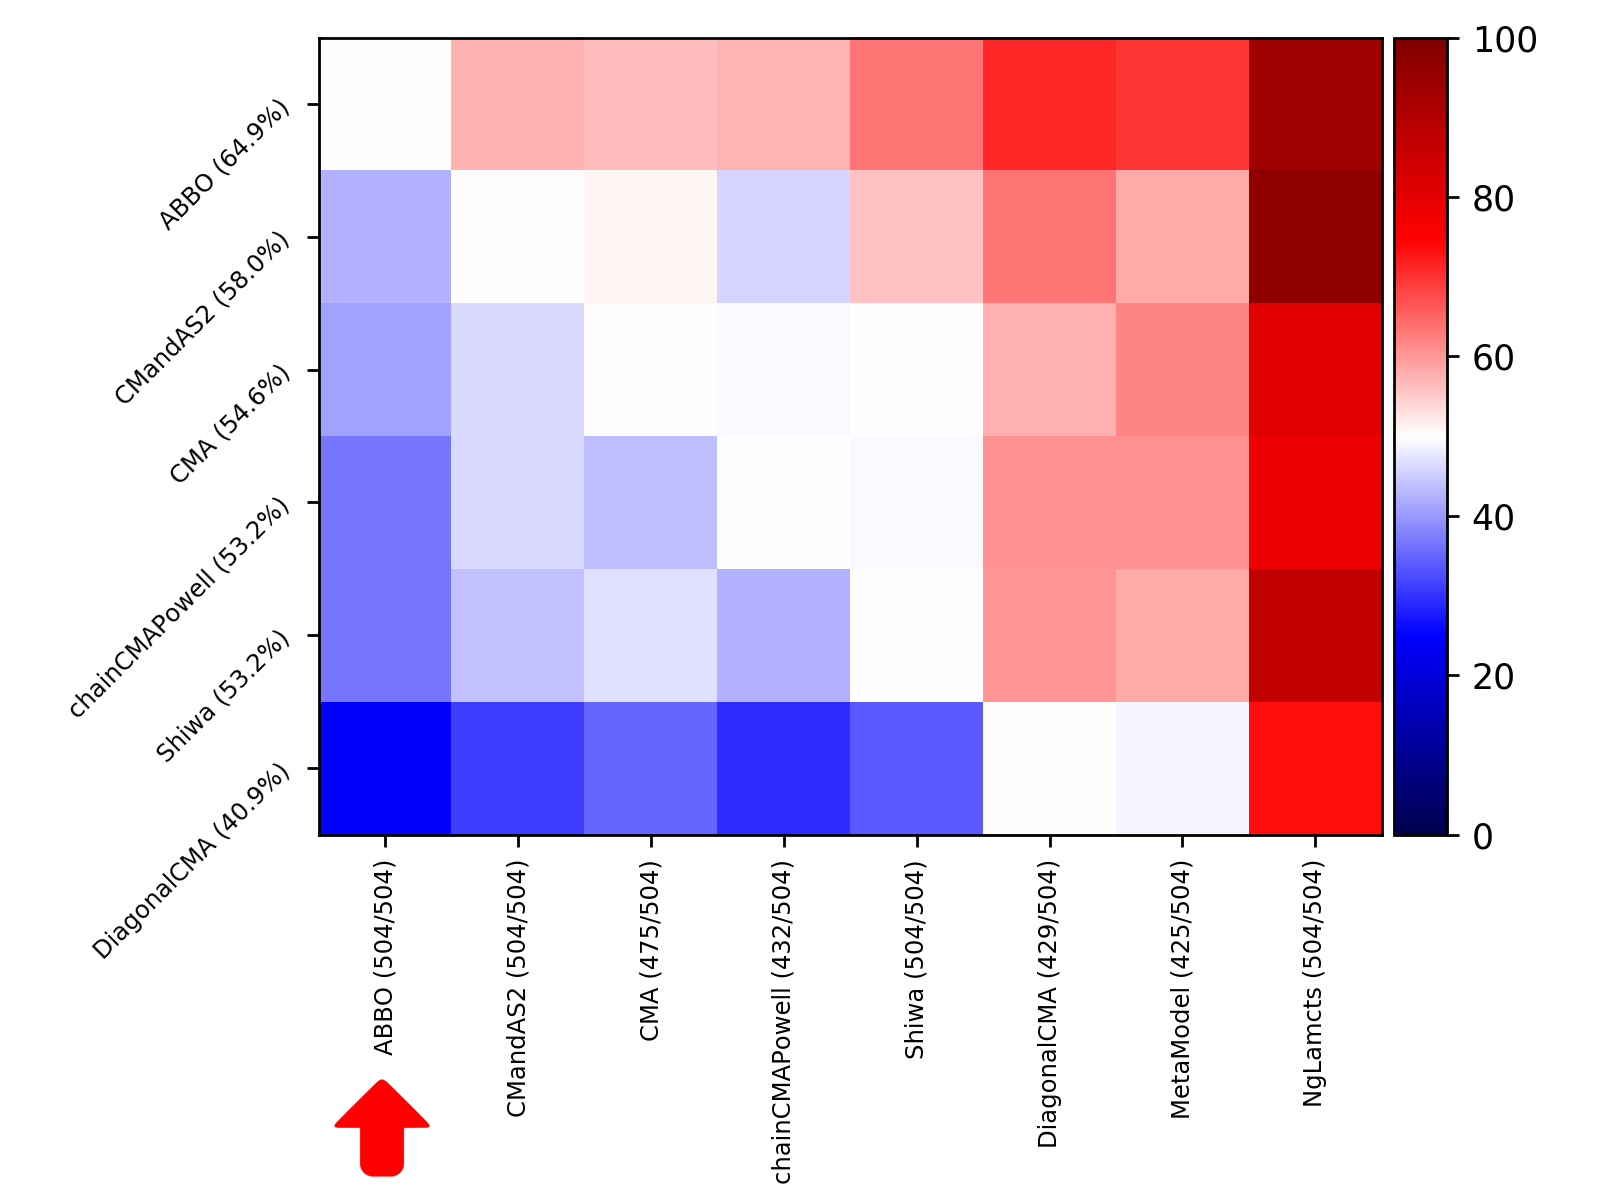
\includegraphics[width=.4\textwidth]{benchmark/fa_yabigbbob.png}
%        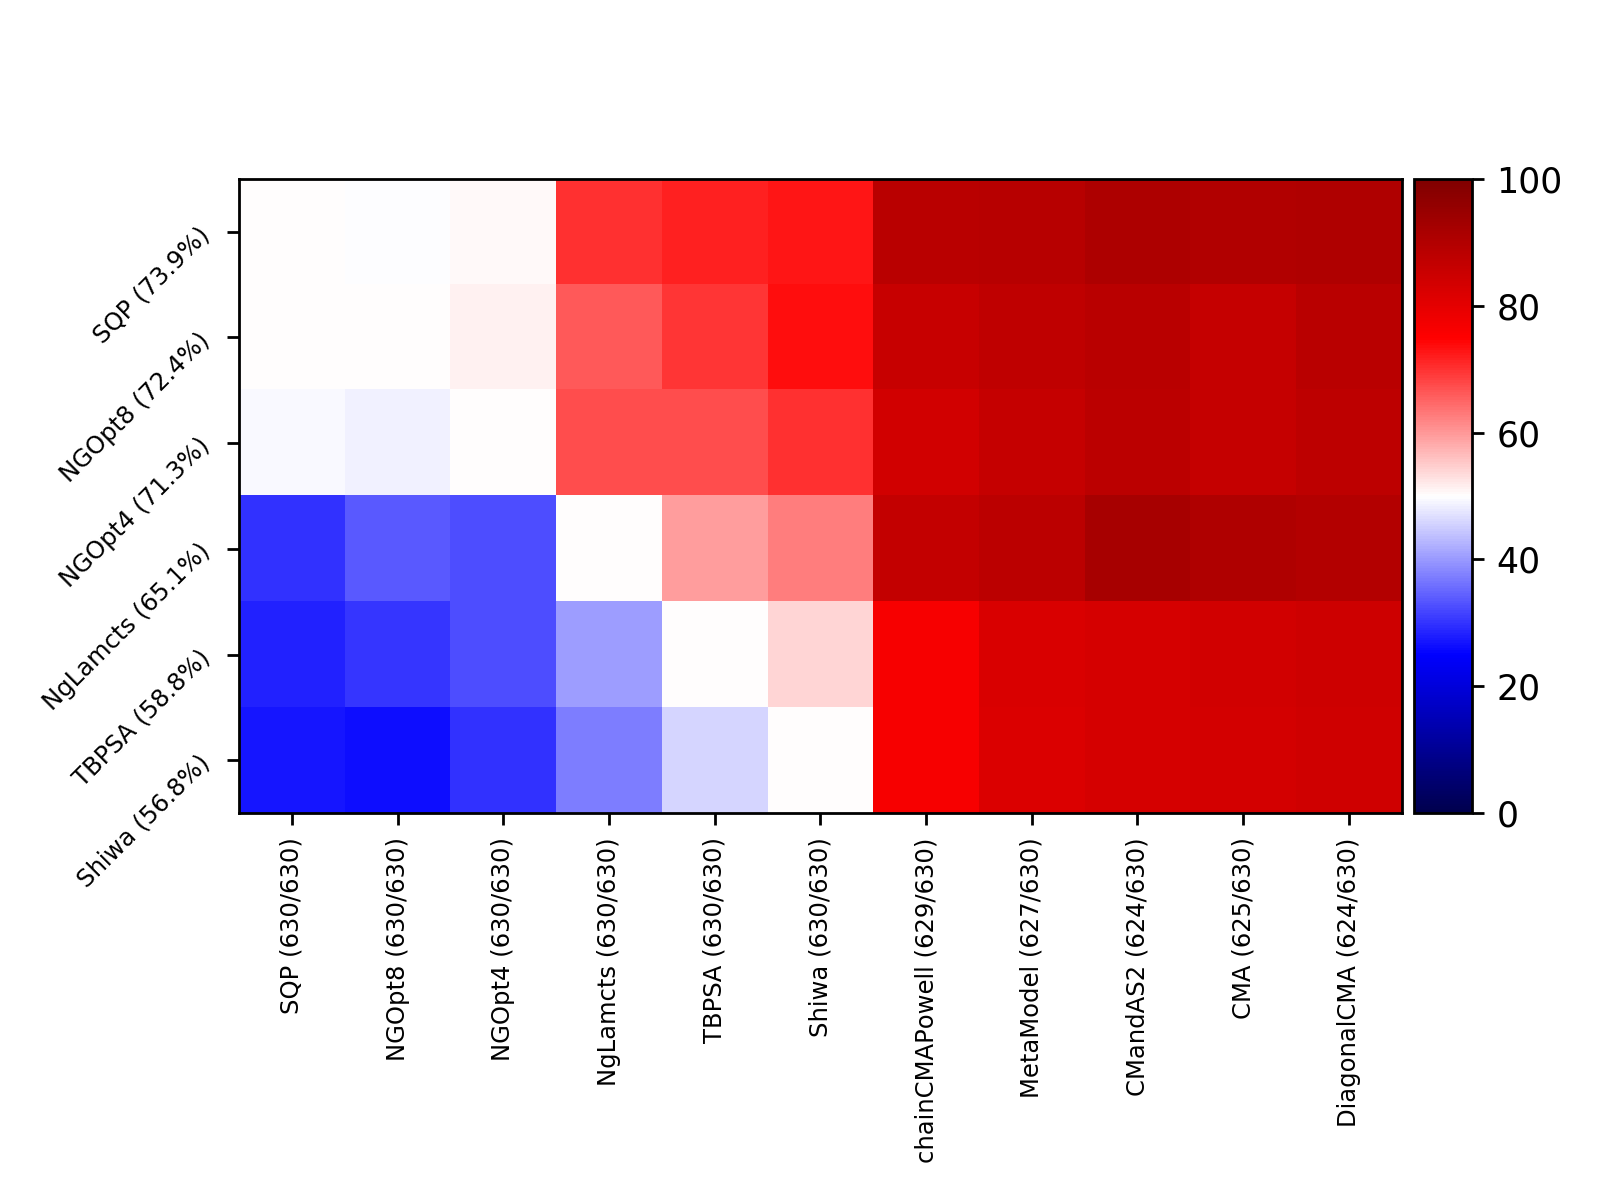
\includegraphics[width=.4\textwidth]{benchmark/fa_yanoisybbob.png}
%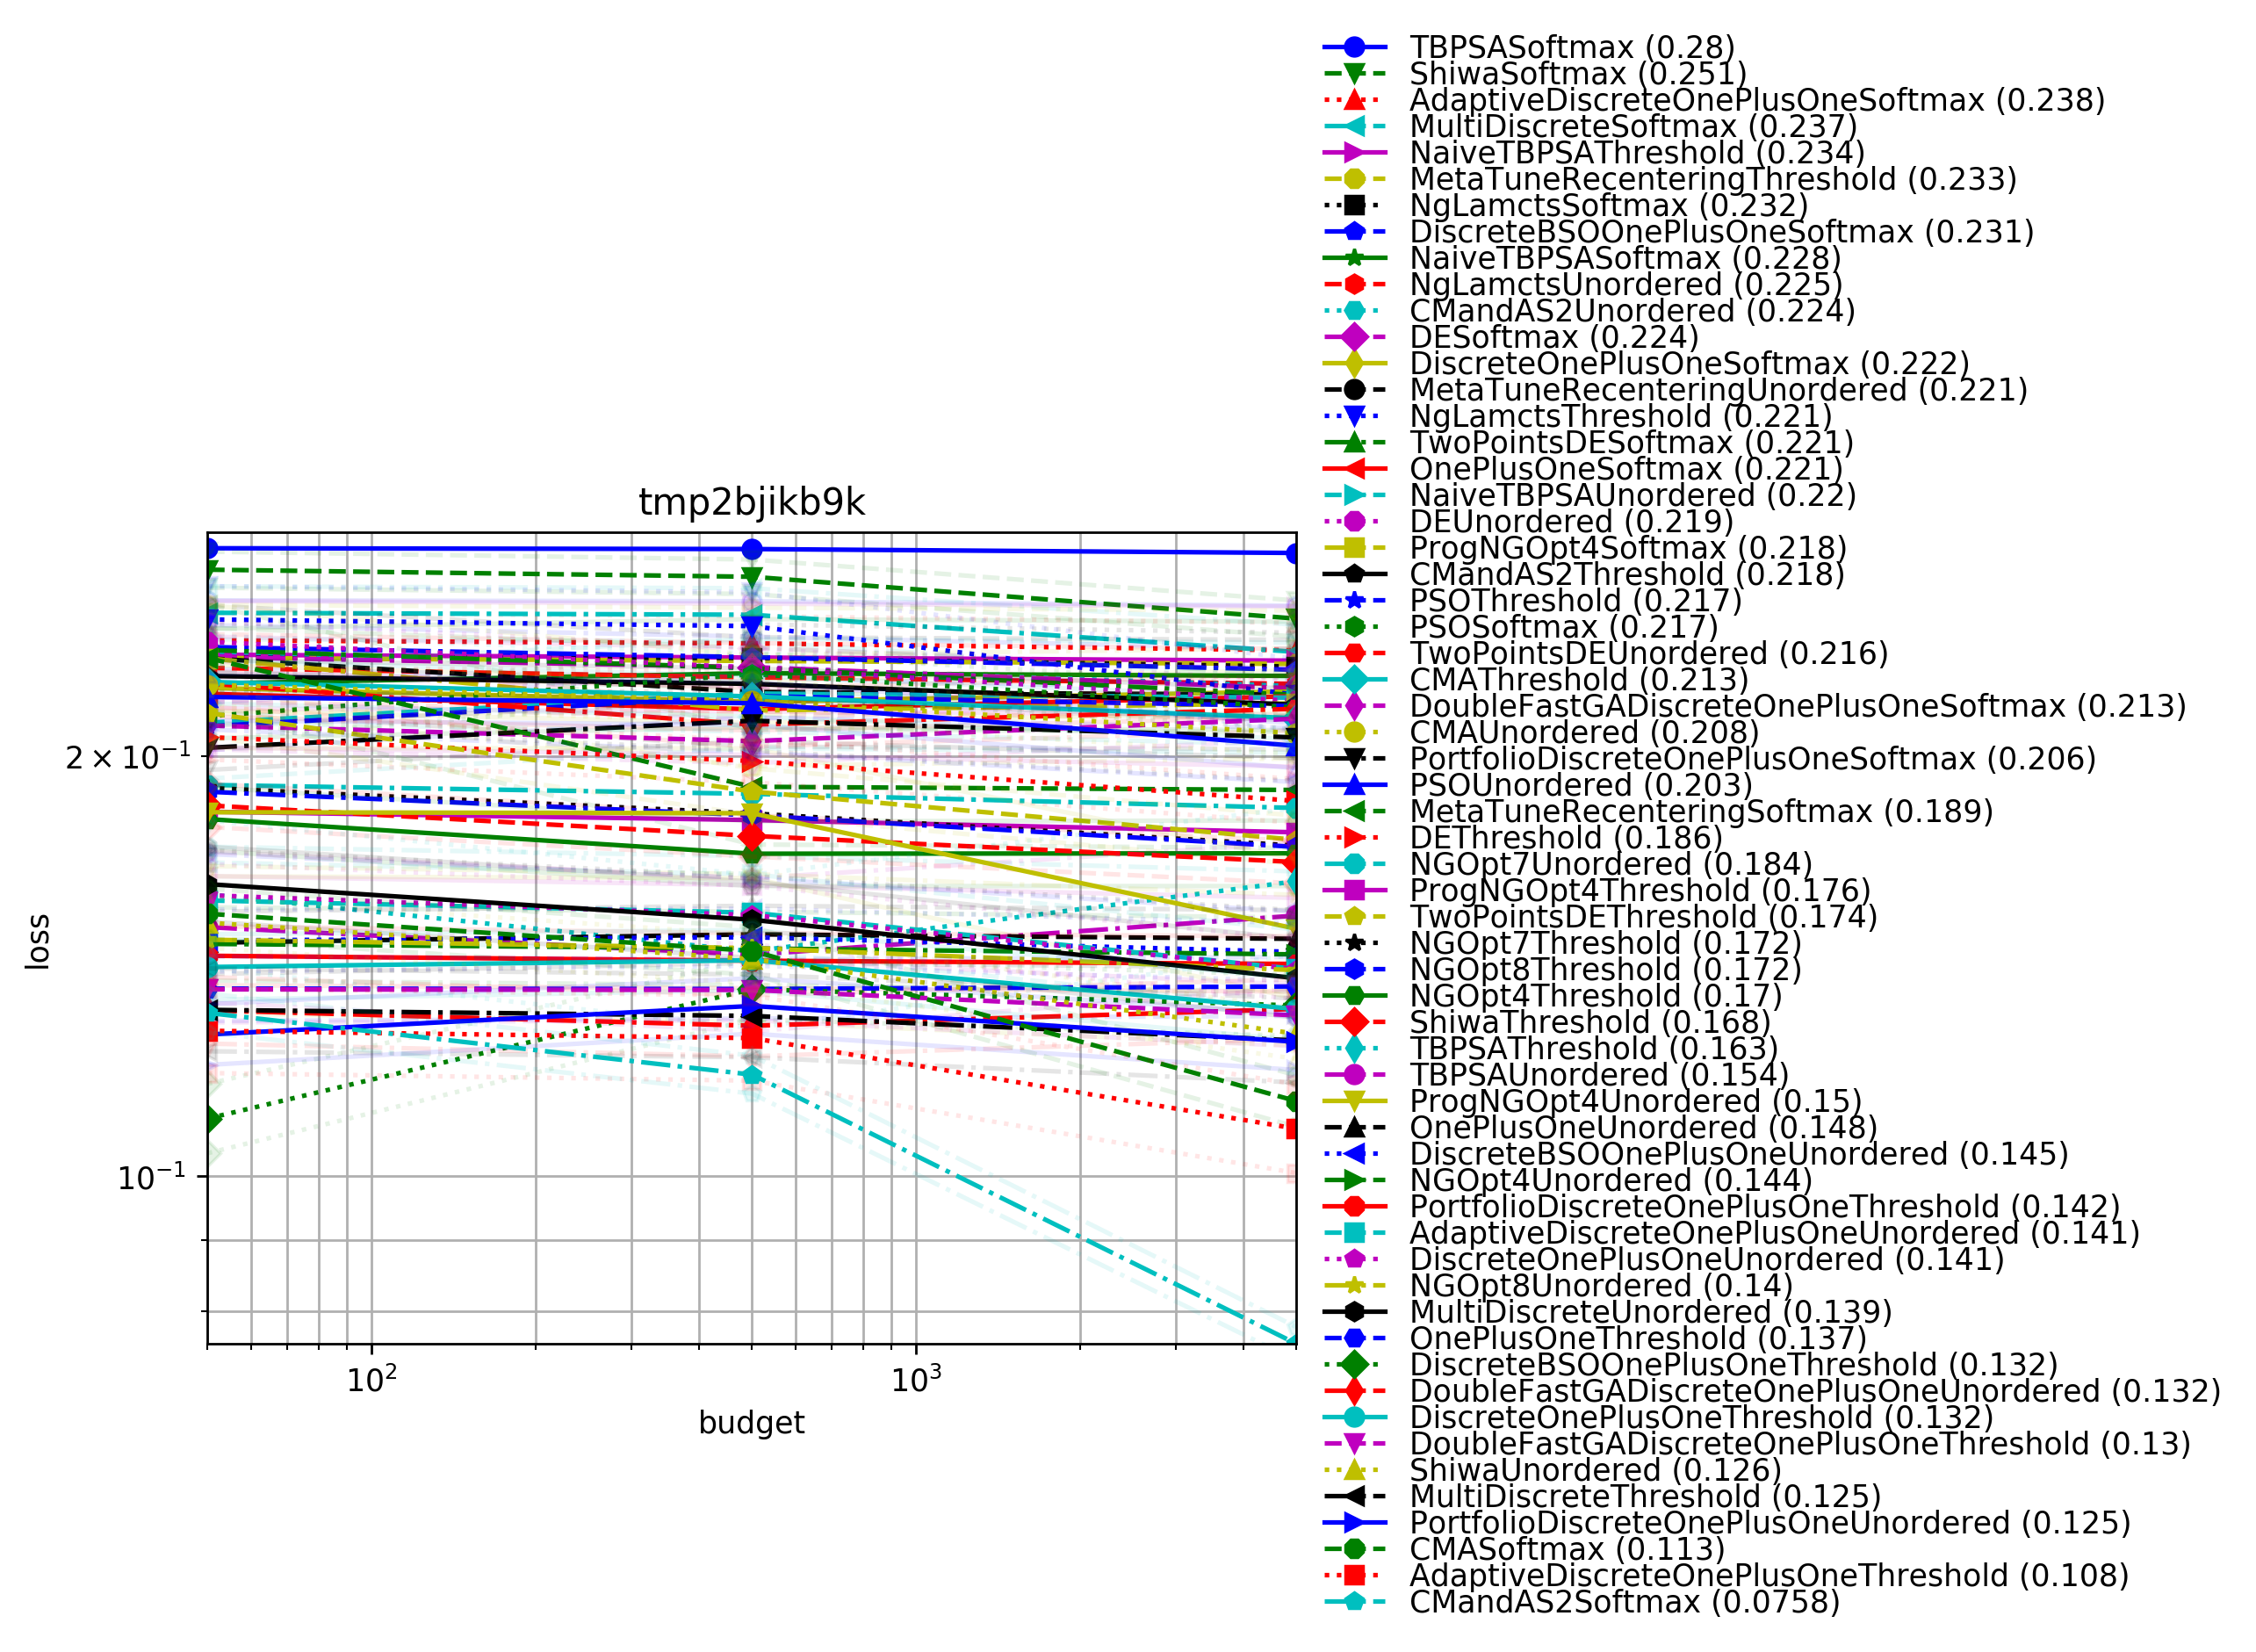
\includegraphics[width=.4\textwidth]{benchmark/xp_instrum_discrete.png}
%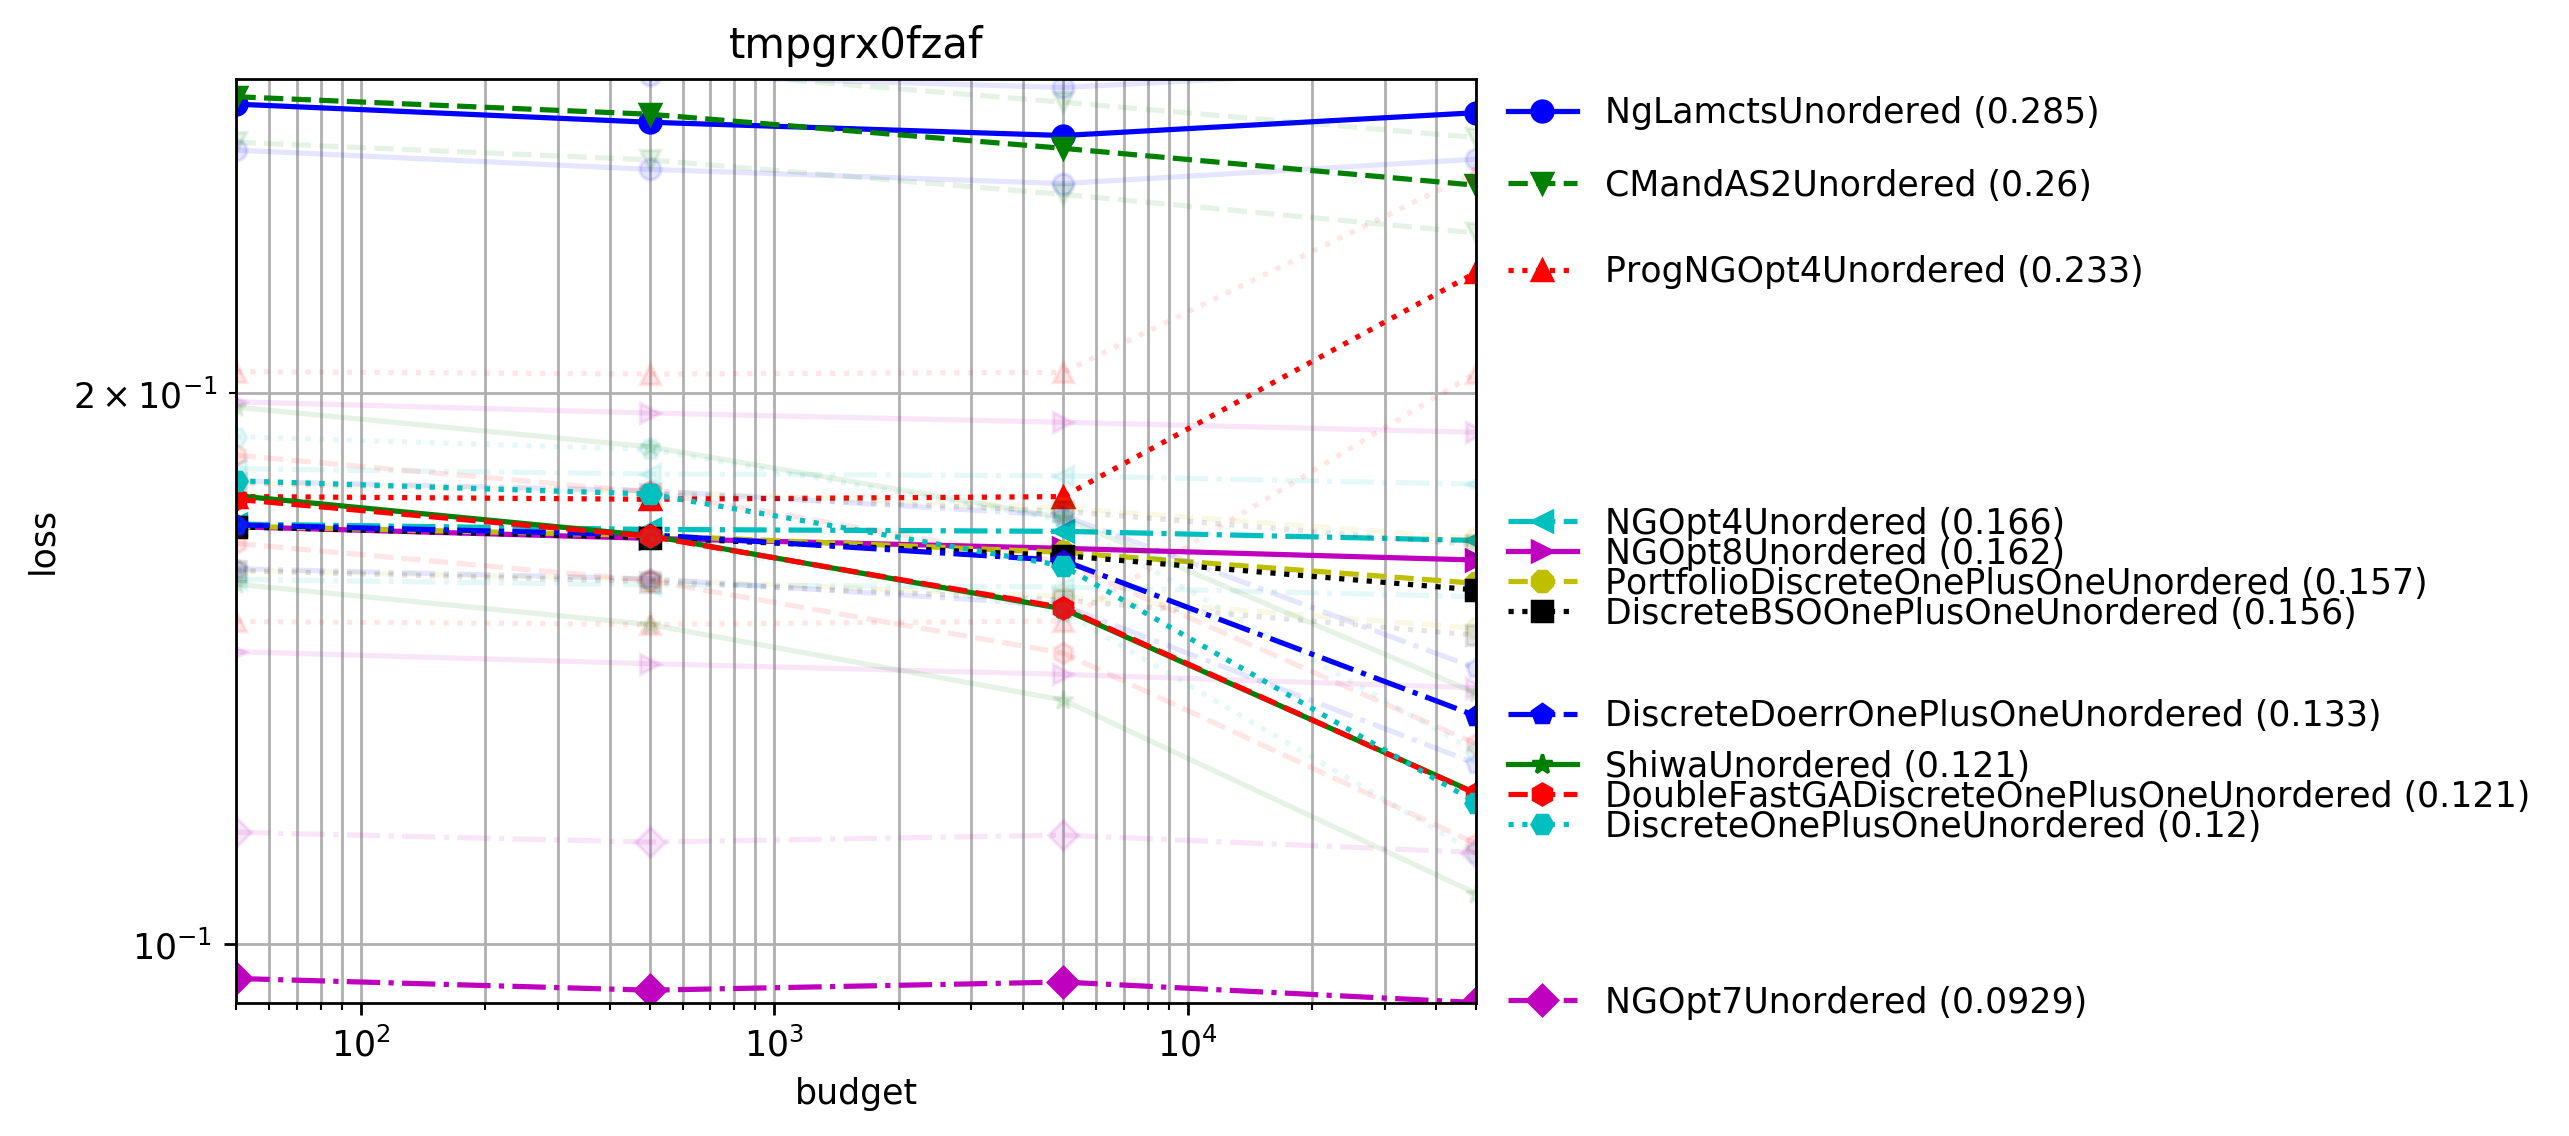
\includegraphics[width=.4\textwidth]{benchmark/xp_sequential_instrum_discrete.png}\\
%%\twocaptions[InstrumDiscrete]{SequentialInstrumDiscrete}
	\caption{Average normalized loss and heatmap for YABBOB. Additional plots for High-dimensional (HD), NoisyHD, and Large budgets are available in Fig.~\ref{bbobfigbis}. Other variants include parallel, differences of budgets, and combinations of those variants, with excellent results for \ngoptq{}.}
    \label{bbobfig}
\end{figure*}
\begin{figure*}[t]
    \centering
\includegraphics[trim={0 0 0 28},clip,width=.58\textwidth]{sections/appendix/h220benchmarks/benchmark/xp_pyomo.png}
\includegraphics[trim={0 0 130 90},clip,width=.4\textwidth]{sections/appendix/h220benchmarks/benchmark/fa_sequential_fastgames.png}
\\%\includegraphics[width=.4\textwidth]{benchmark/fa_photonics.png}\\ 
%	%\onecaption{Photonics}\\
%\twocaptions[Pyomo]{Seq. Fastgames}
	\caption{Additional problems: Pyomo (left figure, covering Knapsack, P-median and others) and SequentialFastgames (on the right, presented as heatmaps due to the high noise. Subsumes GuessWho, War, Batawaf, Flip). Rockets, SimpleTSP, PowerSystems, and LSGO plots are available in Figs.~\ref{figaddrwbis}, and~\ref{figaddrwbisbis}. Pyomo and SimpleTSP include discrete variables. Pyomo includes constraints. Rocket, PowerSystems, SequentialFastGames are based on open source simulators.}
	\label{figaddrw}
\end{figure*}


\label{b2}
{\textbf{AllDEs and Hdbo}} are {benchmark collections specifically designed to compare DE variants (AllDEs) and high-dimensional Bayesian Optimization (Hdbo), respectively~\cite{nevergrad}.} %comparisons with benchmarks specifically designed for DE variants (All DEs) and high-dimensional Bayesian Optimization (Hdbo).
These benchmark functions are similar to the ones used in YABBOB. % though not equal.
Many variants of DE (resp. BO) are considered.
Results are presented in  Fig.~\ref{specif}. They show that the performance of \ngoptq{}, relatively to DE or BO, is consistent over a wide range of parametrizations of DE or BO, at least in their most classical variants, which are all available in Nevergrad for empirical comparisons. 
%\subsubsection{Benchmarking for an optimum far away}
% {\textbf{Far-optimum:}}
% \label{b3}
% \cite{farcsa} pointed out the importance of being able to quickly adapt to areas with a smooth improvement direction. Therefore, benchmarks with an optimum far from zero can be interesting. We add such a feature, directly inspired from \cite{farcsa}, in \nevergradnewbranch{} and compare some optimization algorithms in Fig.~\ref{faroptim}. 

{\textbf{Realworld:}}
\label{b4}
%The Realworld optimization benchmark was proposed in \cite{nevergrad}, it includes testbeds from \cite{mlda} and \cite{versatile}. We present experiments in Fig.~\ref{figrw}. They show that \ngoptq{} performs well also on benchmarks never used for defining it, and on real-world functions. 
{A test of \ngoptq{} is performed on the Realworld optimization benchmark suite proposed in~\cite{nevergrad}. This suite includes testbeds from MLDA~\cite{mlda} and from~\cite{versatile}. Results for this suite, presented in  Fig.~\ref{figrw}, confirm that \ngoptq{} performs well also on benchmarks that were not explicitly used for its design. However, this benchmark was used for designing Shiwa, which was the starting point for the design of \ngoptq{}. A rigorous cross-validation, on benchmarks {totally} independent from the design of Shiwa, is provided in {the} next sections.}

\subsection{New Benchmark Suites Used Only for Evaluating \ngoptq{}}% and others}

% \begin{figure}[t]
%     \centering
% \includegraphics[trim={0 0 0 28},clip,width=.58\textwidth]{benchmark/xp_pyomo.png}
% \includegraphics[trim={0 0 130 90},clip,width=.4\textwidth]{benchmark/fa_sequential_fastgames.png}
% \\%\includegraphics[width=.4\textwidth]{benchmark/fa_photonics.png}\\ 
% %	%\onecaption{Photonics}\\
% %\twocaptions[Pyomo]{Seq. Fastgames}
% 	\caption{Additional problems: Pyomo (covering Knapsack, P-median and others) SequentialFastgames (presented as heatmaps due to the high noise: GuessWho, War, Batawaf, Flip). Rockets, SimpleTSP, PowerSystems and LSGO plots are available in Appendix~\ref{addfig}, Figures~\ref{figaddrwbis} and~\ref{figaddrwbisbis}. Pyomo and SimpleTSP include discrete variables. Pyomo includes constraints. Rocket, PowerSystems, SequentialFastGames are based on open source simulators and are already merged from \nevergradnewbranch{} to Nevergrad.}
% 	\label{figaddrw}
% \end{figure}

{\textbf{ Pyomo}}\label{b5}
 is a modeling language in Python for optimization problems~\cite{pyomo}.
It has been adopted for formulating large models for complex and real-world systems, including energy systems and network resource systems.
We implemented an interface to Pyomo for Nevergrad. % and enriched our benchmark problems~\cite{source}, which include discrete variables and constraints.
Experimental results are summarized in Fig.~\ref{figaddrw}. They show that \ngoptq{} also performs decently in discrete settings and in constrained cases. %note{is this also cross-validation? Or did you use this to refine \ngoptq{}? OT: this is cross-validation}


% \begin{figure}[t]
%     \centering
%     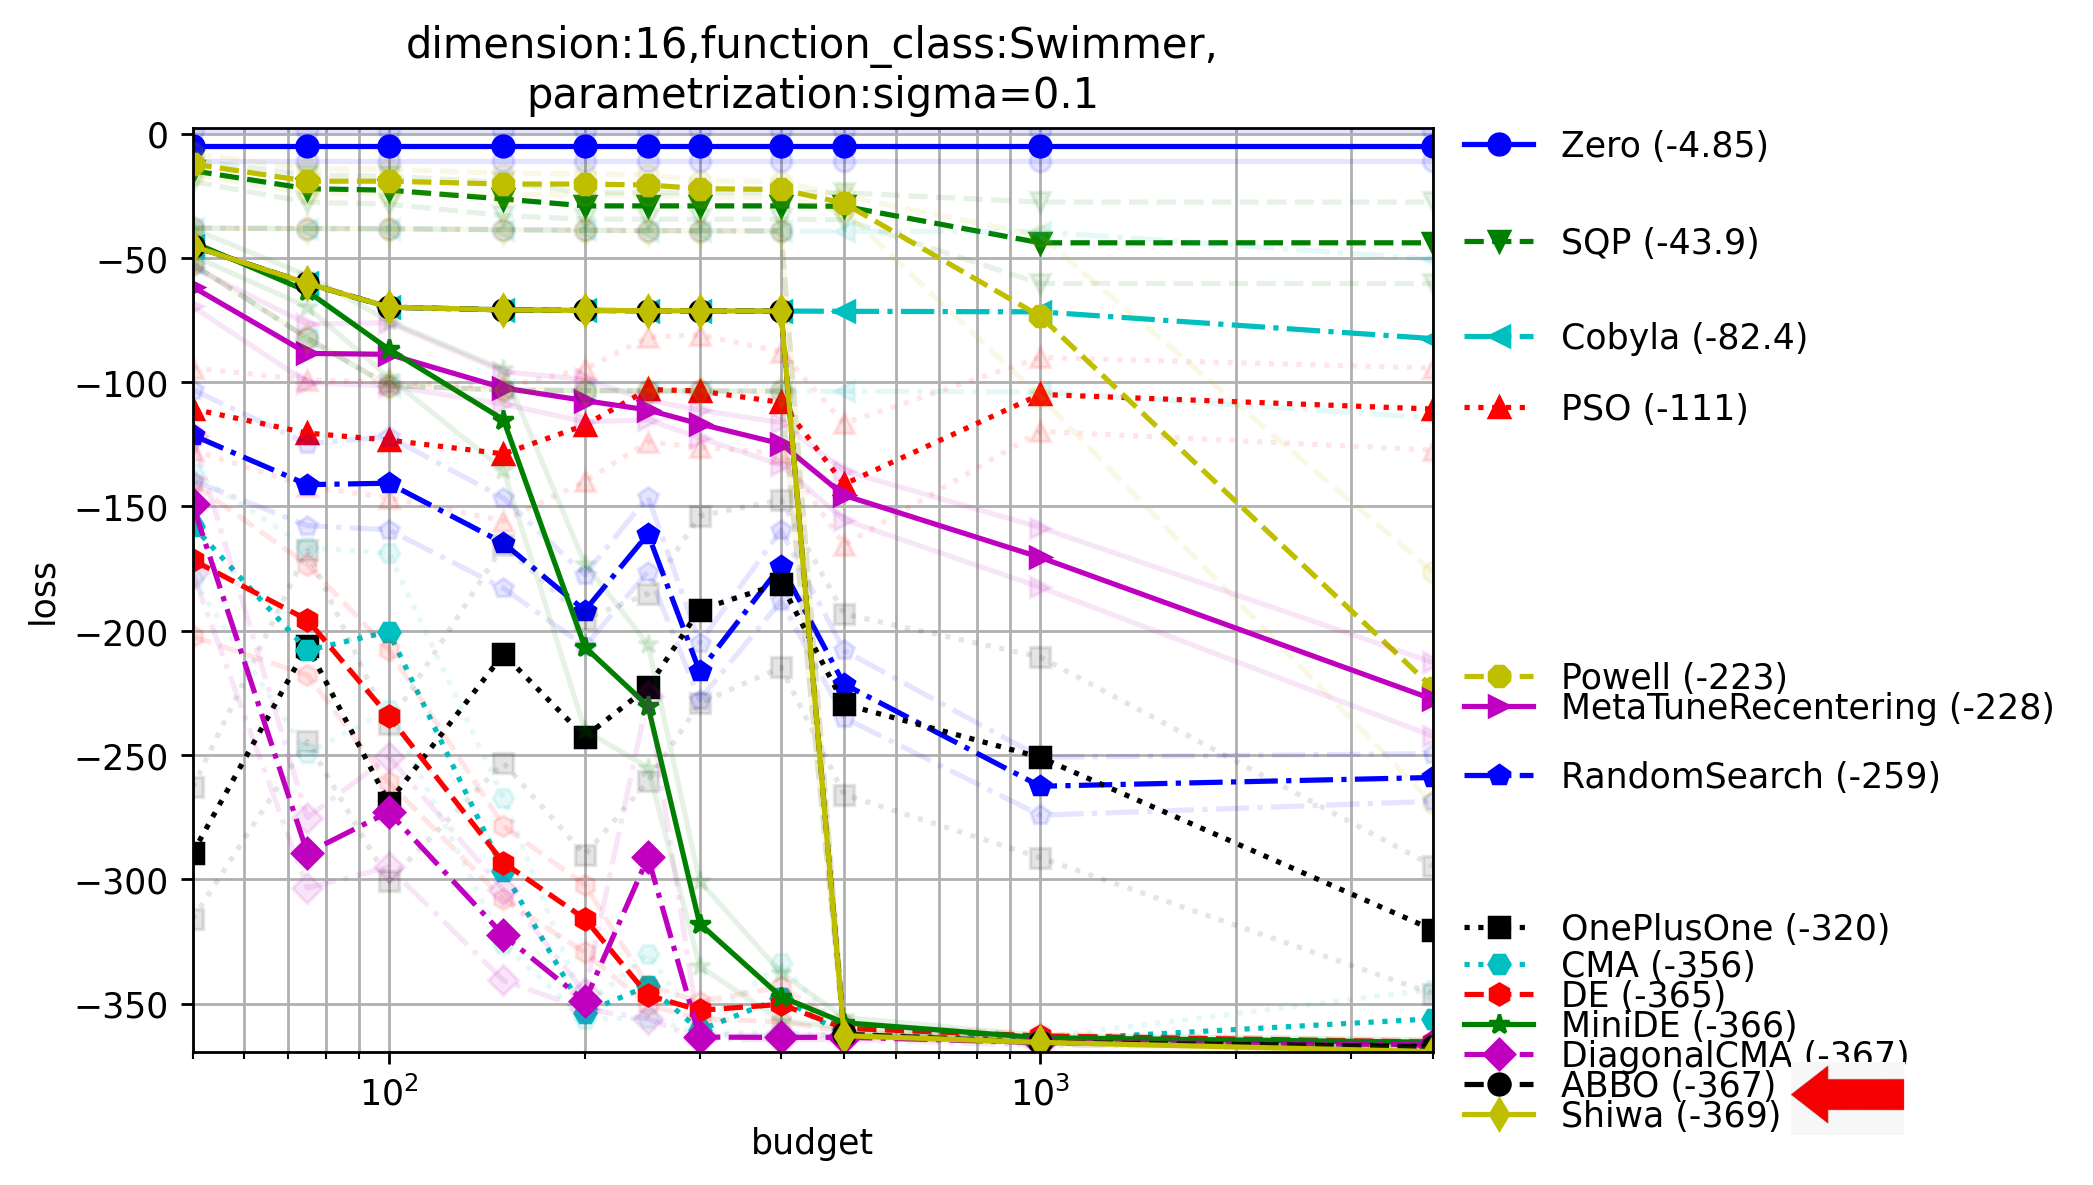
\includegraphics[width=.49\textwidth]{benchmark/control_problem/xpresults_dimension16,function_classSwimmer,parametrizationsigma=0.1.png}
%     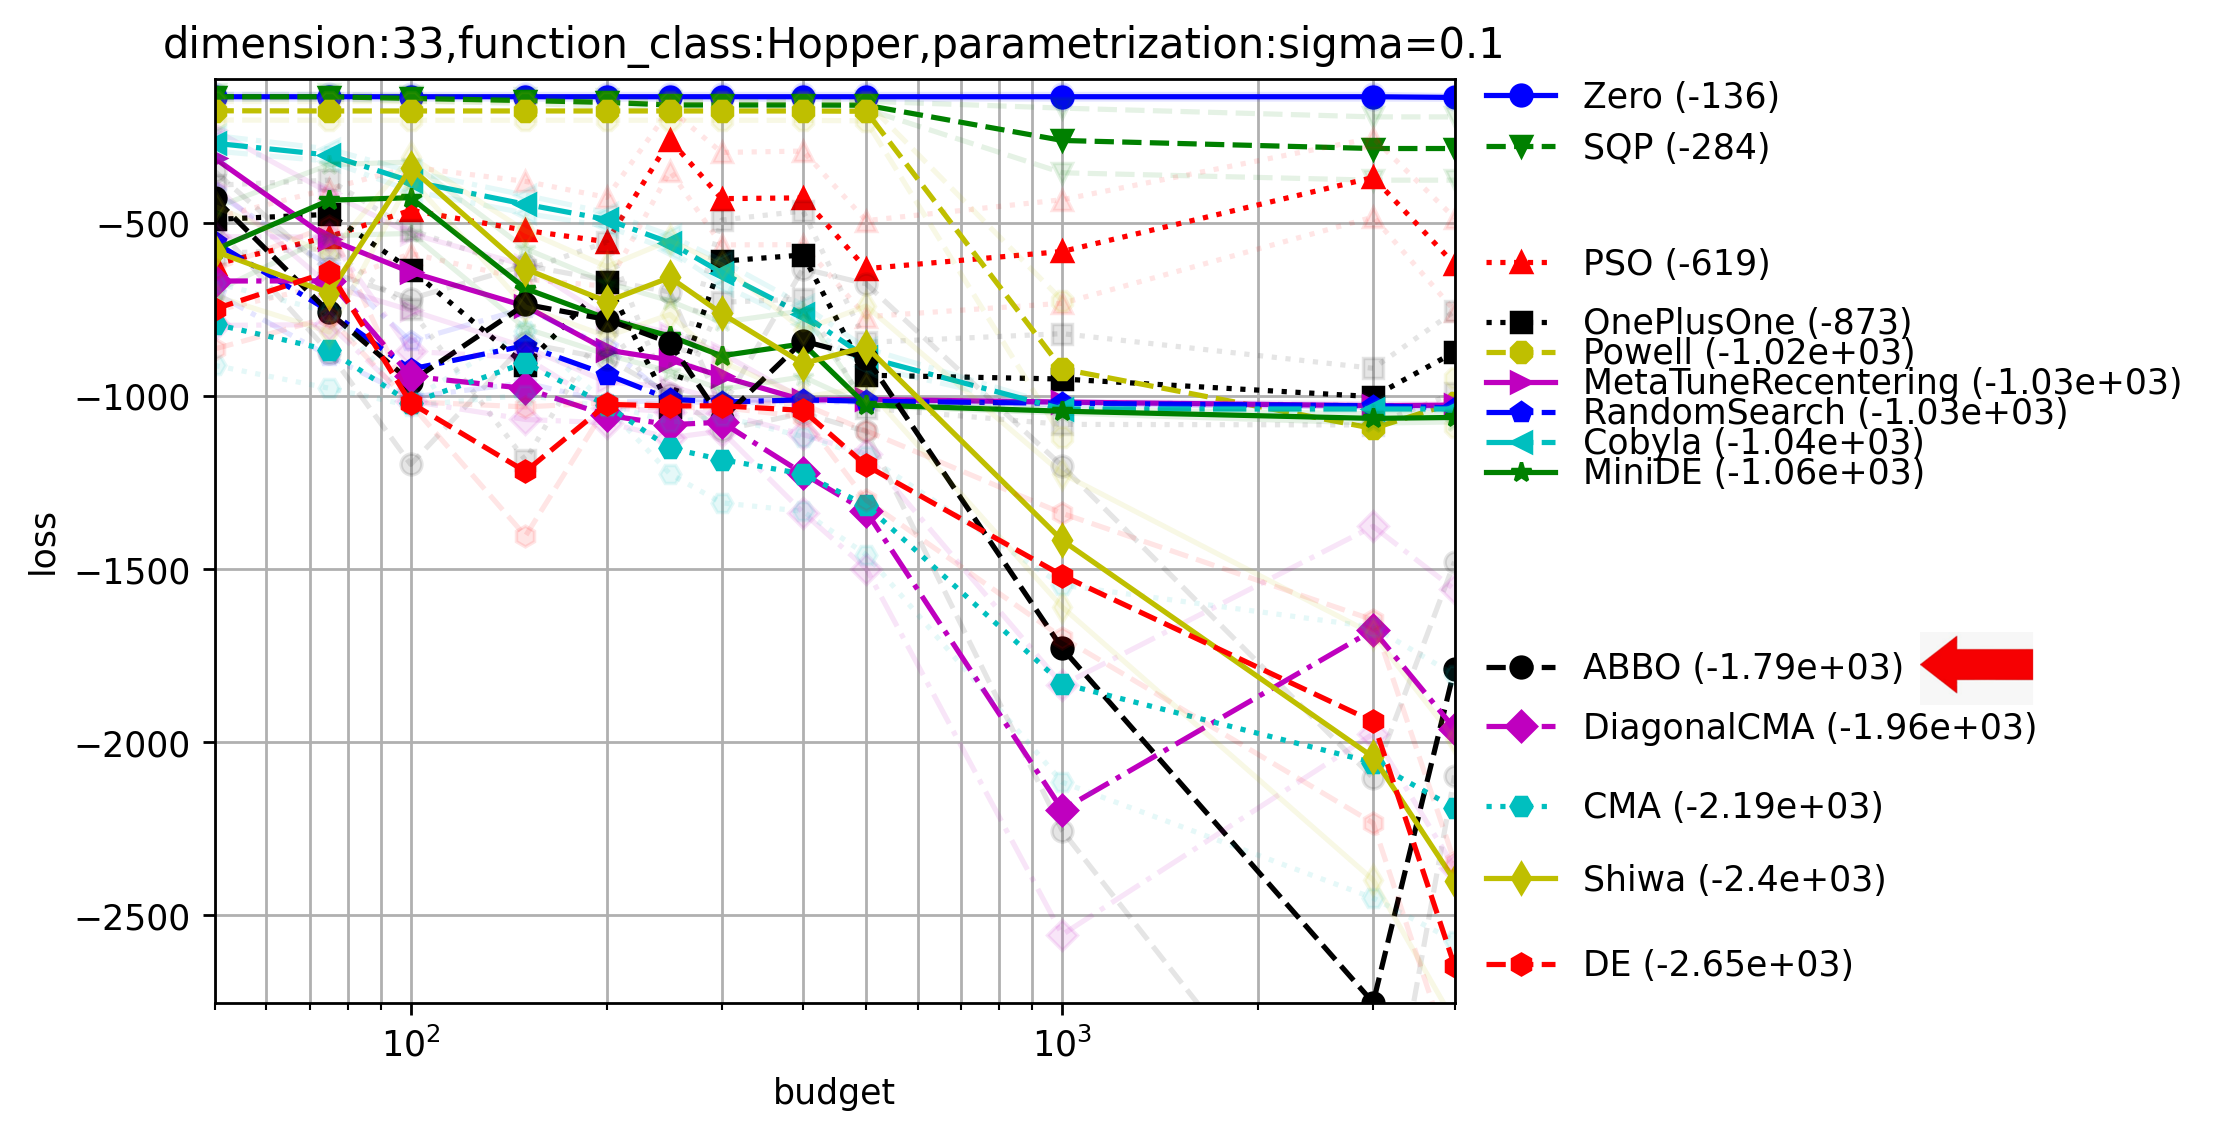
\includegraphics[width=.49\textwidth]{benchmark/control_problem/xpresults_dimension33,function_classHopper,parametrizationsigma=0.1.png}\\
%      %\twocaptions[Swimmer (dim 16)]{Hopper (dim 33)}
%     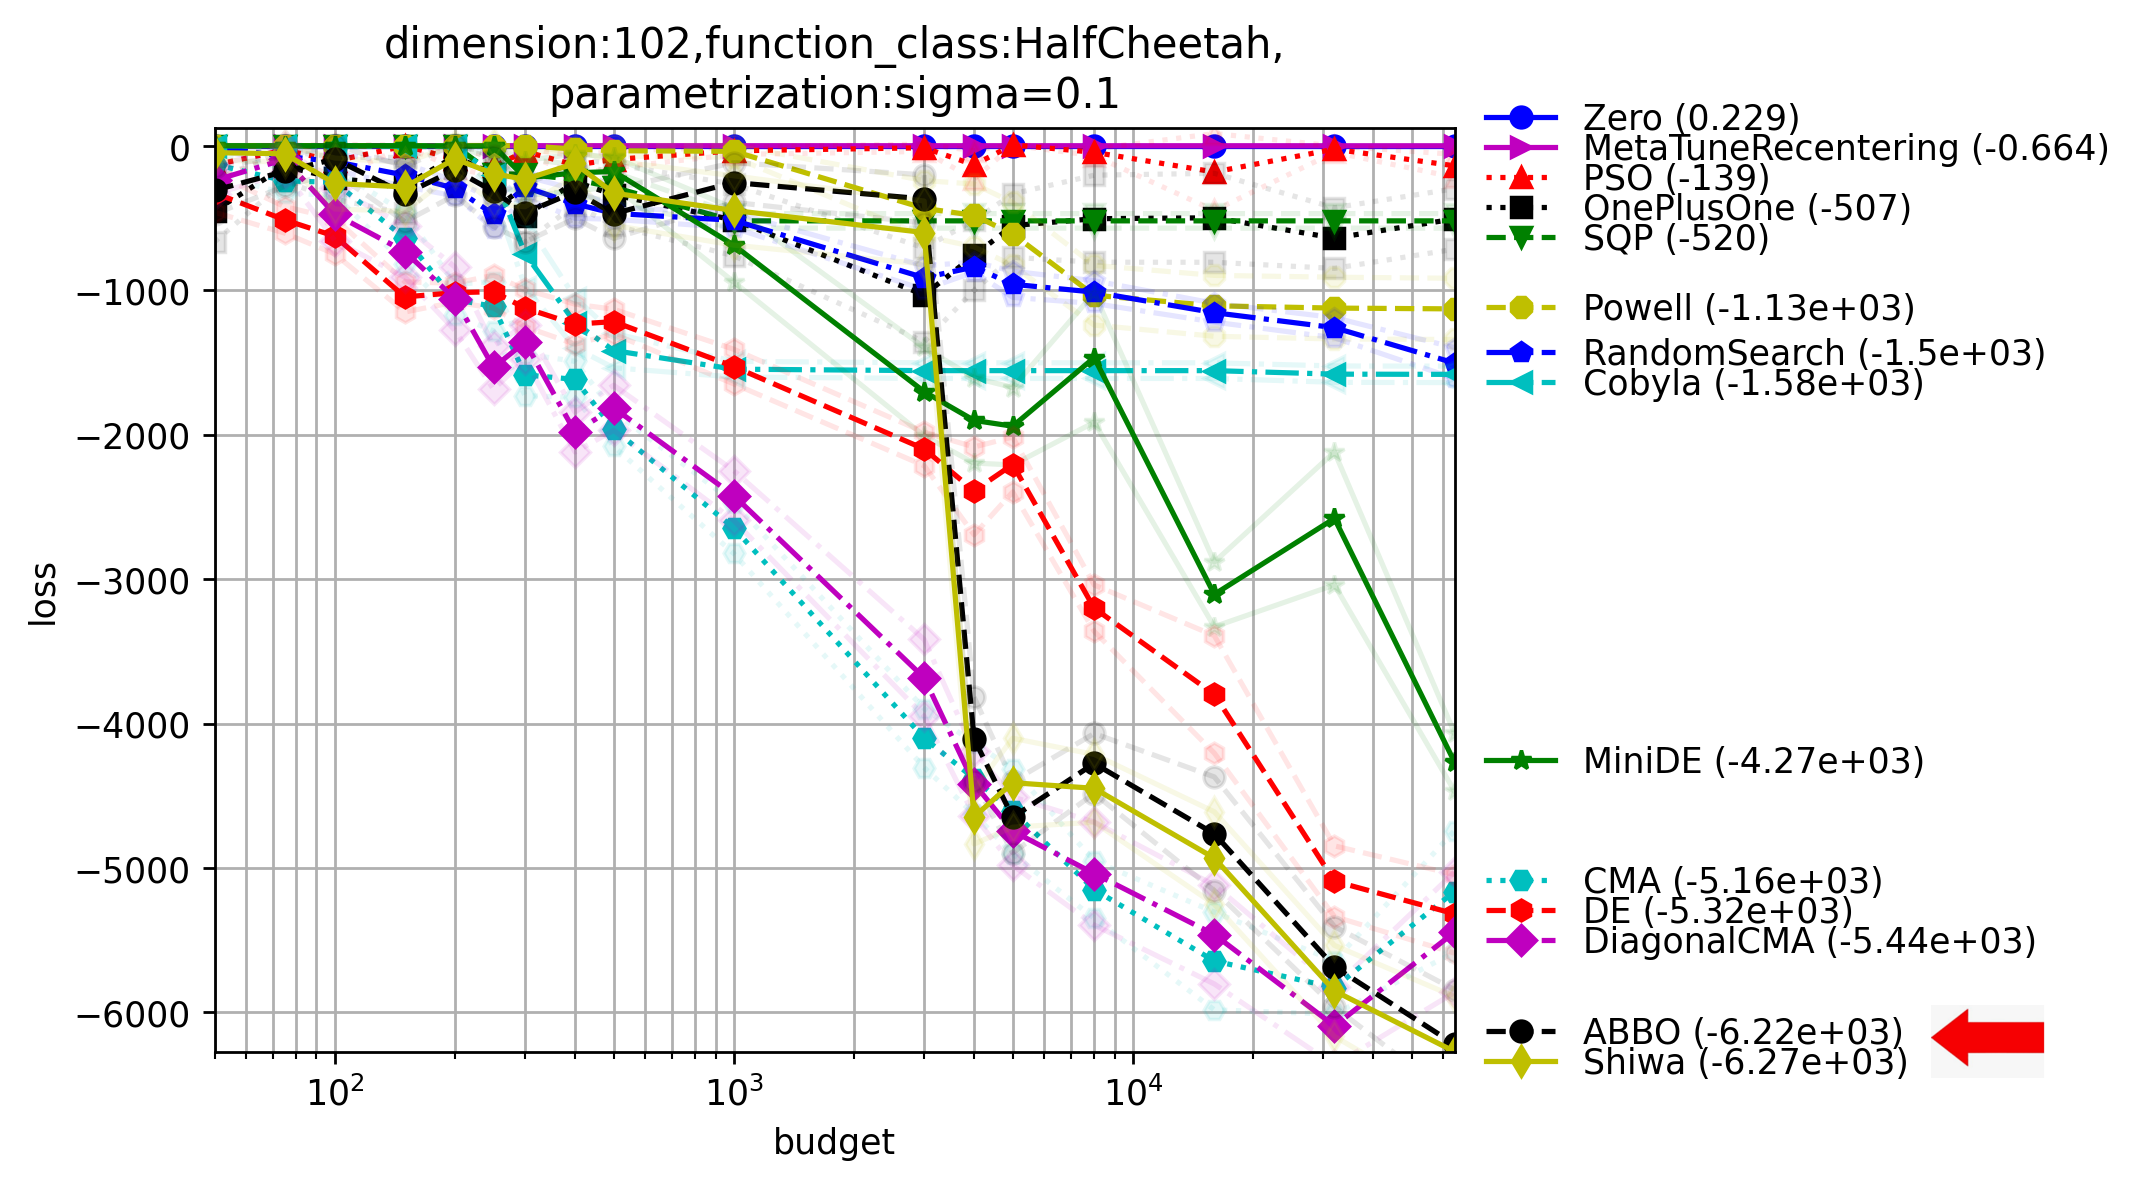
\includegraphics[width=.48\textwidth]{benchmark/control_problem/xpresults_dimension102,function_classHalfCheetah,parametrizationsigma=0.1.png}
%     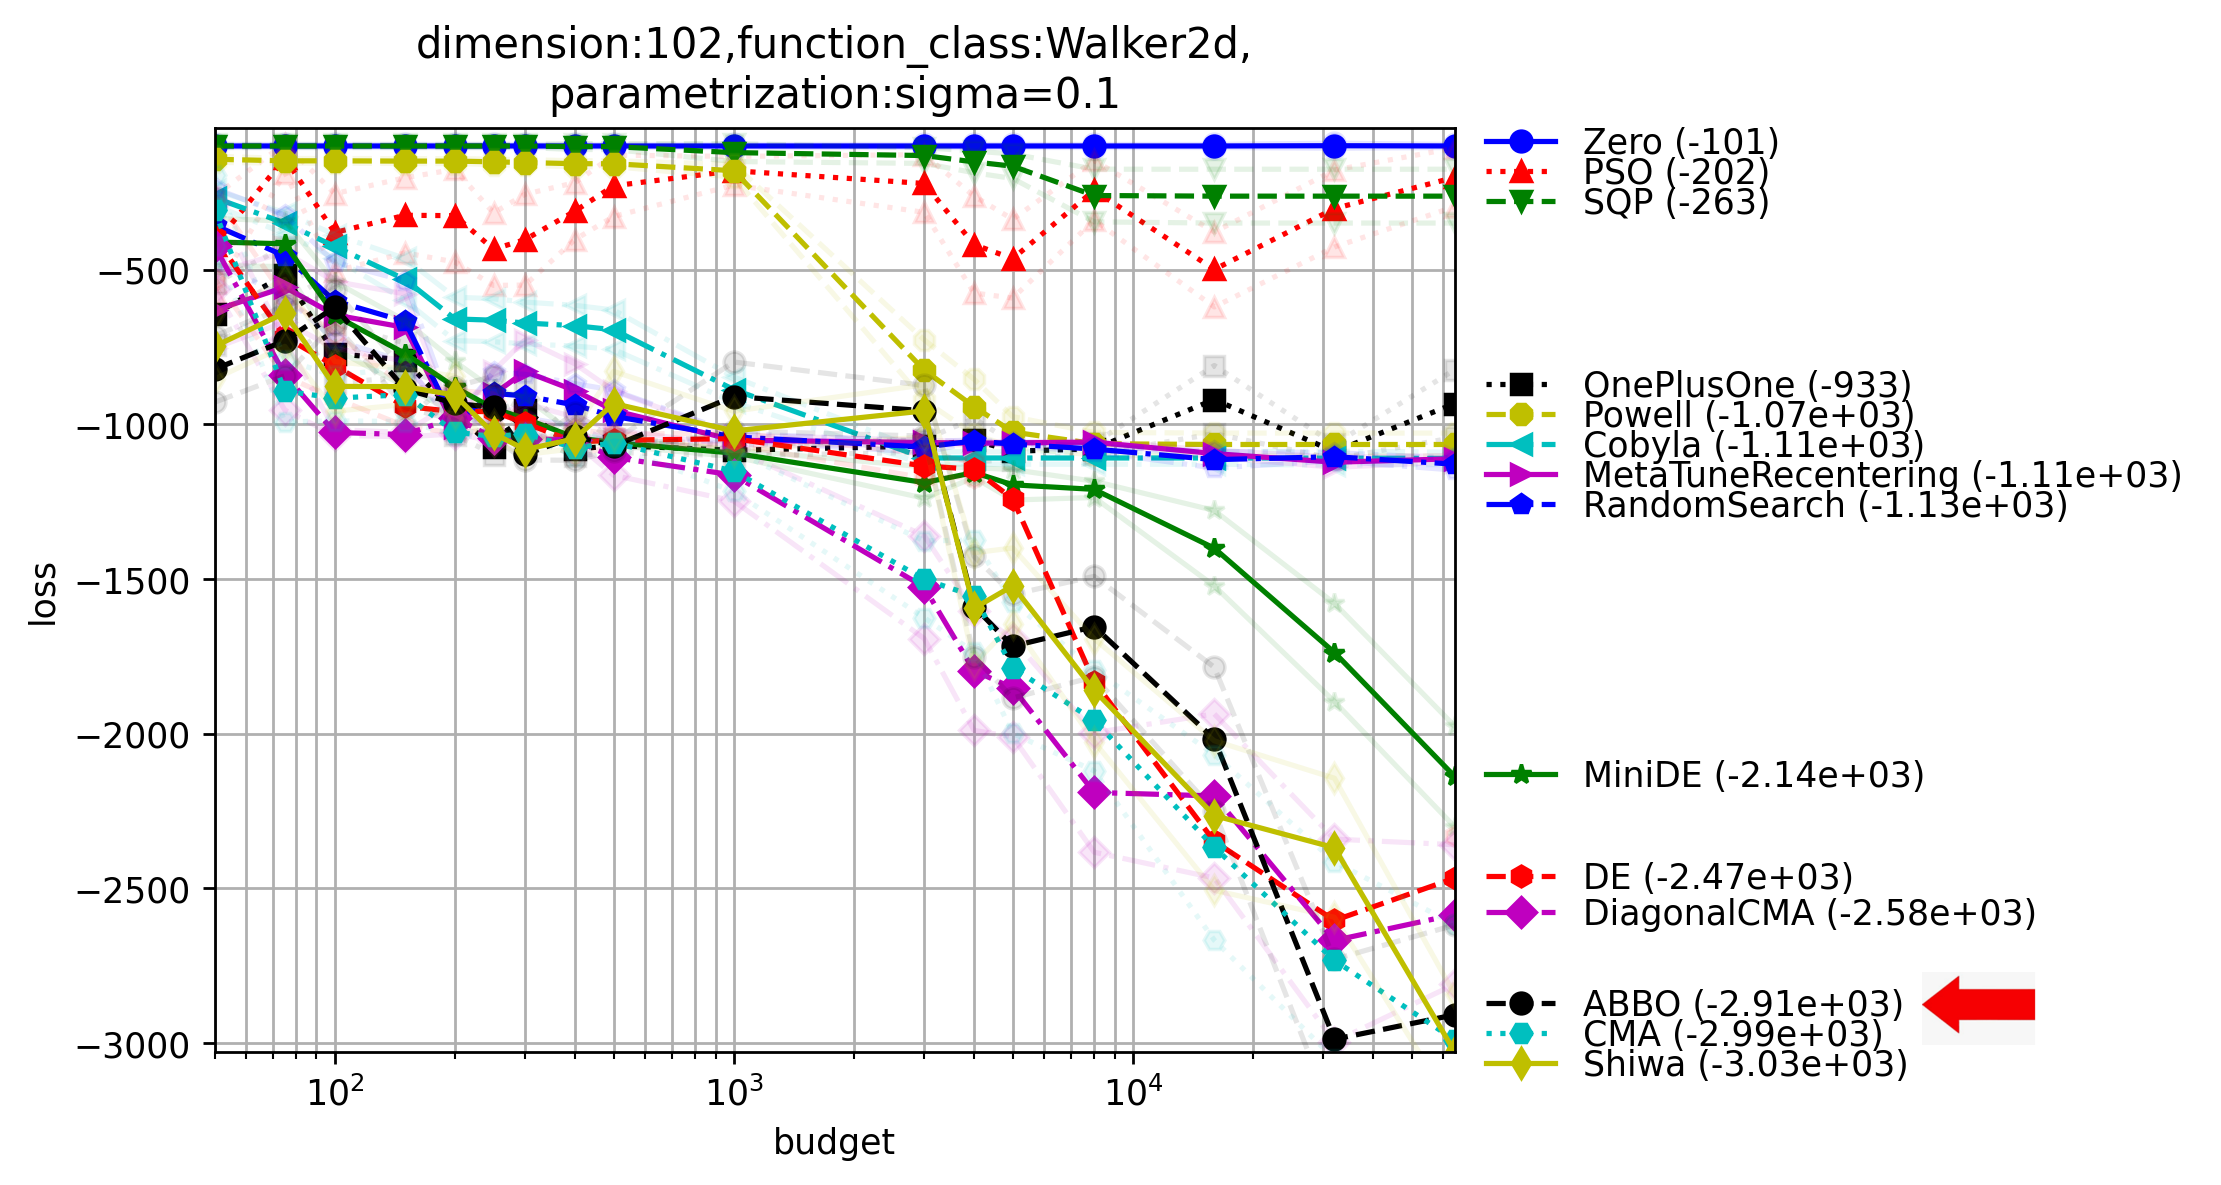
\includegraphics[width=.49\textwidth]{benchmark/control_problem/xpresults_dimension102,function_classWalker2d,parametrizationsigma=0.1.png}\\
%     %\twocaptions[Half-Cheetah (dim 102)]{Walker-2d (dim 102)}
%         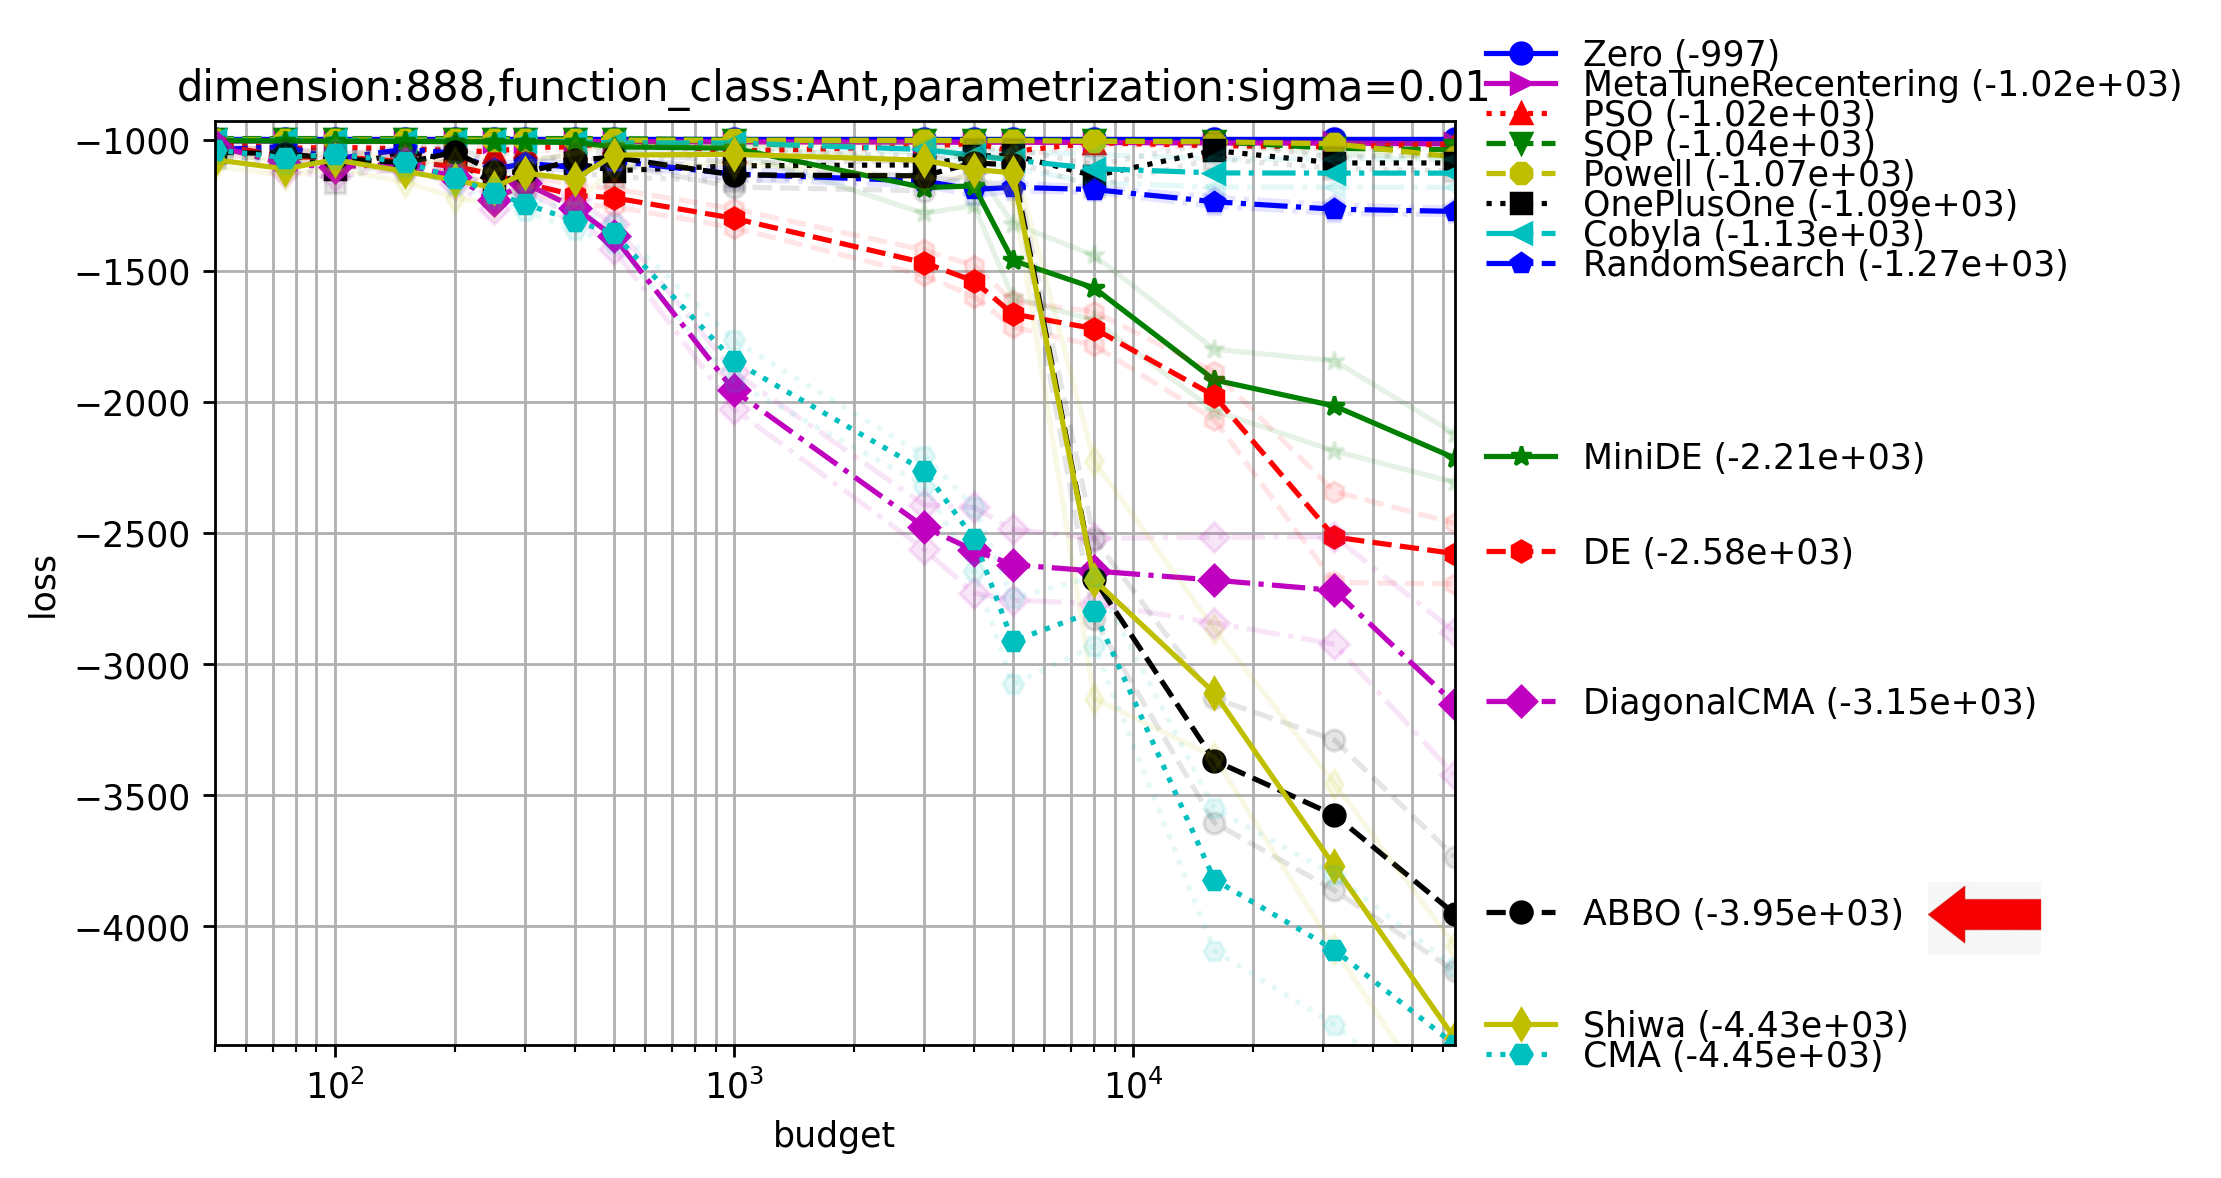
\includegraphics[width=.49\textwidth]{benchmark/control_problem/xpresults_dimension888,function_classAnt,parametrizationsigma=0.01.png}
%     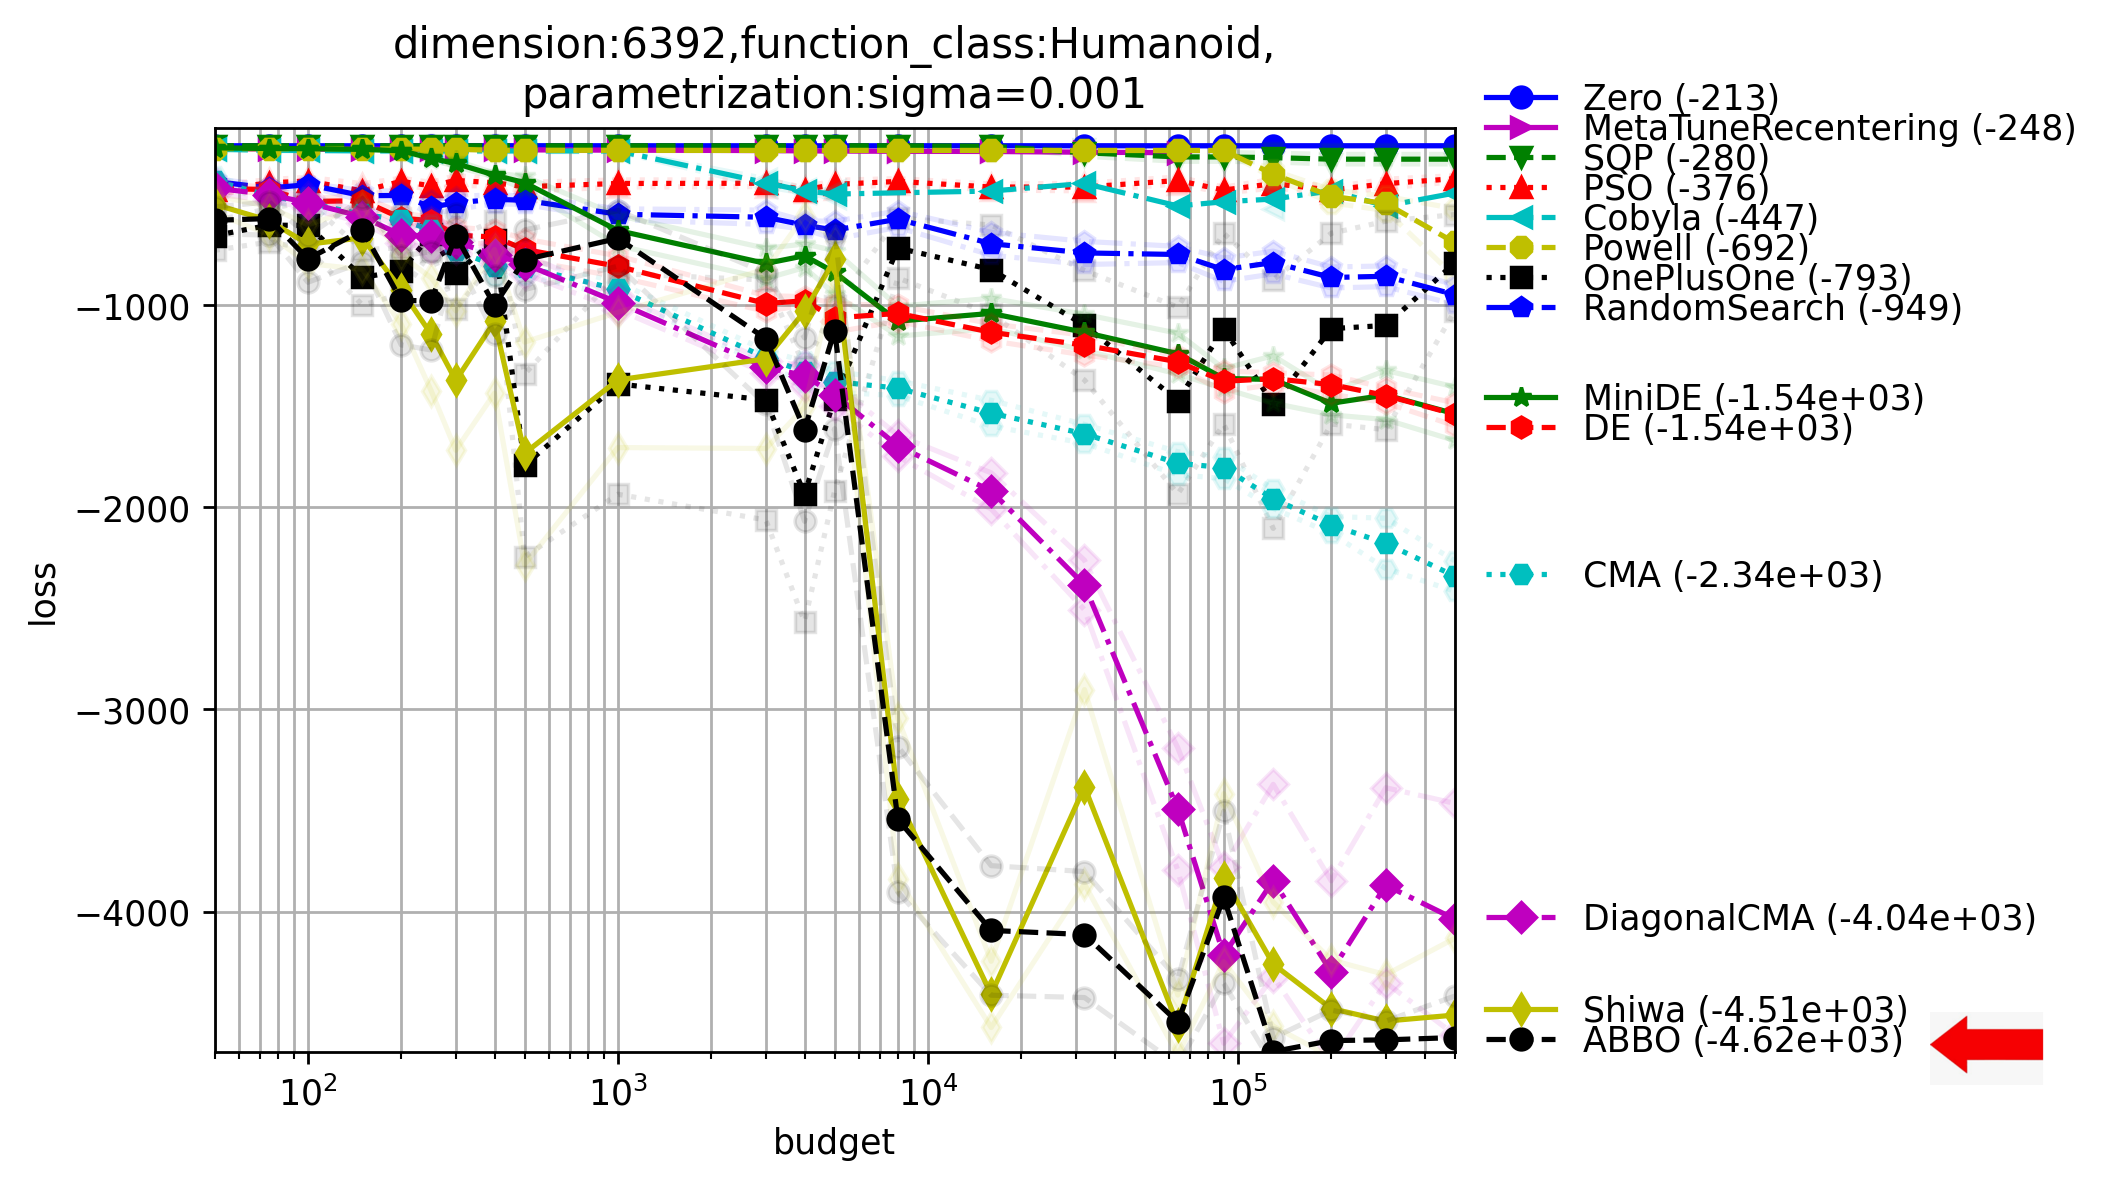
\includegraphics[width=.49\textwidth]{benchmark/control_problem/xpresults_dimension6392,function_classHumanoid,parametrizationsigma=0.001.png}\\
%     %\twocaptions[Ant (dim 888)]{Humanoid (dim 6392)}
% 	\caption{Results on the MuJoCo testbeds. Dashed lines show the standard deviation. Compared to the state of the art in \cite{lamcts}, with an algorithm adapted manually for the different tasks, we get overall better results for Humanoid, Ant, Walker, worse for Swimmer (could match if we had modified our code for the 3 easier tasks as done in \cite{lamcts}), similar for Hopper and Cheetah: we reach the target for 5 of the 6 problems, whereas previous black-box algorithms solved 3 tasks at best. }
%     \label{figMuJoCobis}
% \end{figure}


\begin{figure*}[t]
    \centering
    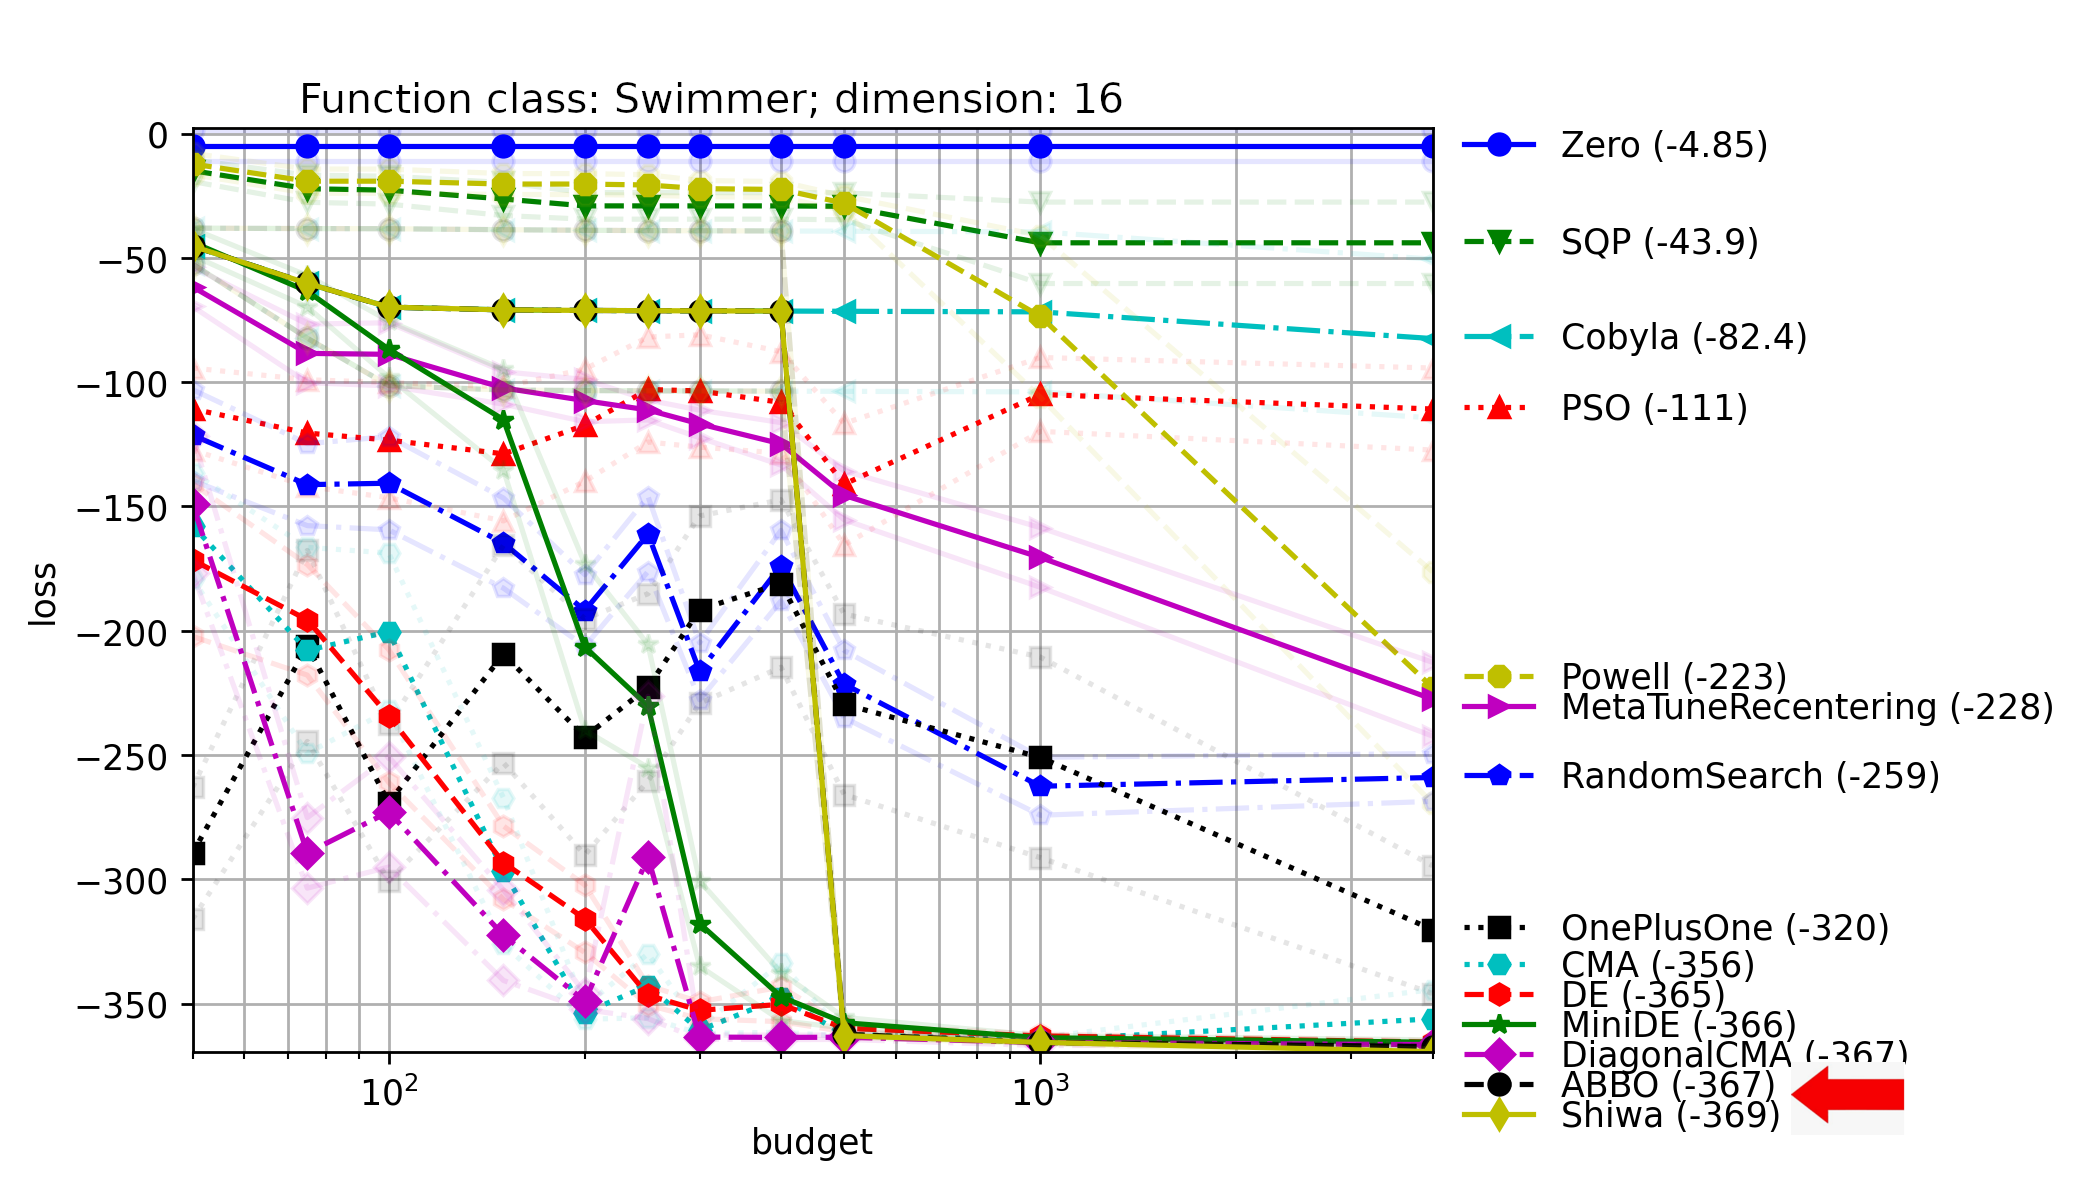
\includegraphics[width=.48\textwidth]{sections/appendix/h220benchmarks/benchmark/control_problem/xpresults_dimension16,function_classSwimmer,parametrizationsigma=0.1_edited.png}
    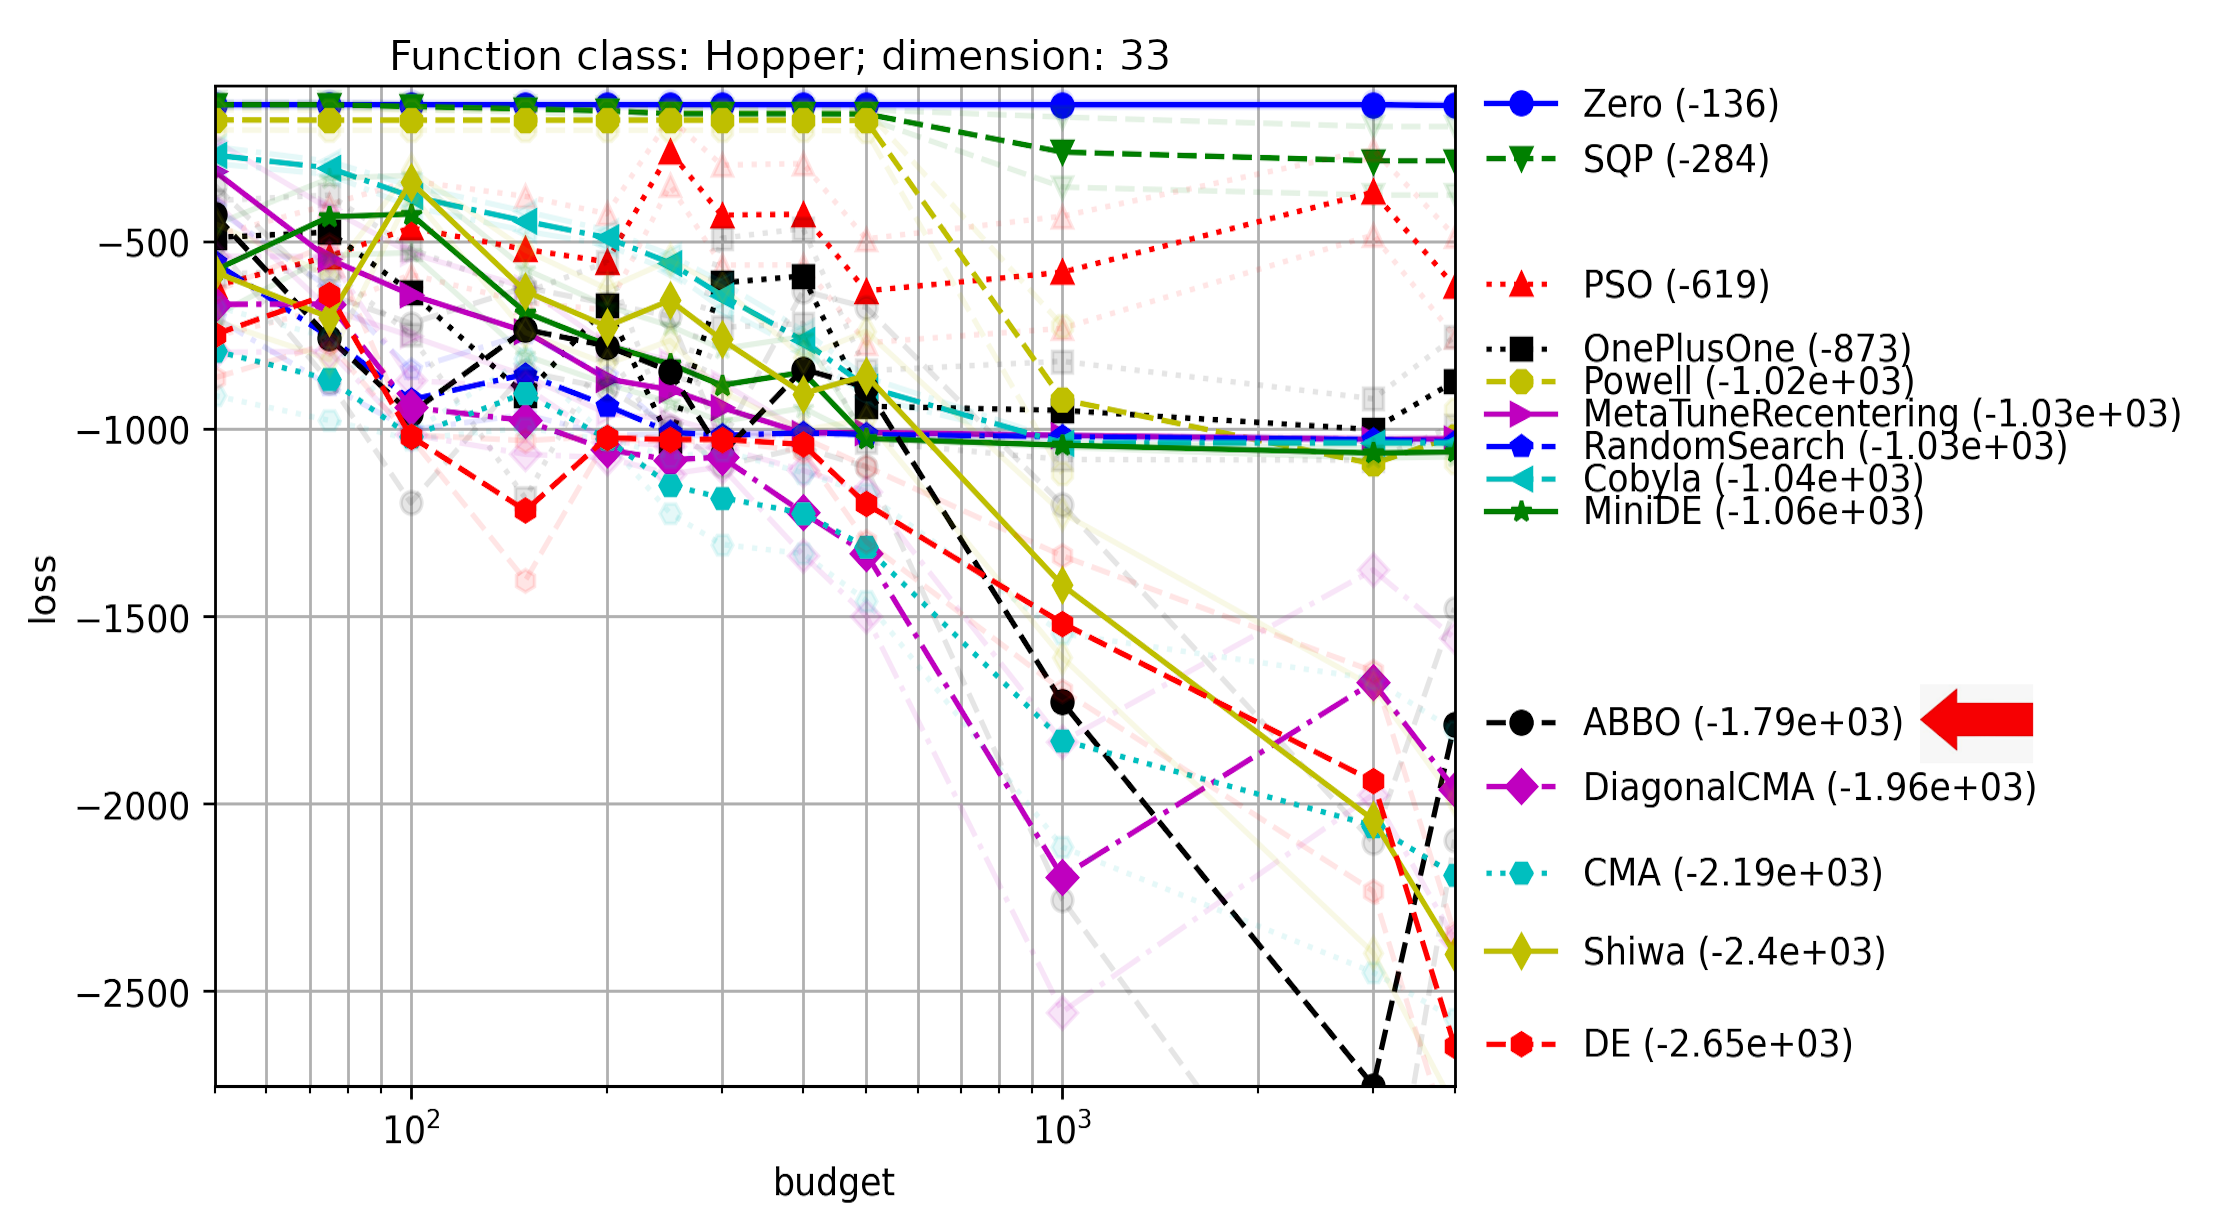
\includegraphics[width=.48\textwidth]{sections/appendix/h220benchmarks/benchmark/control_problem/xpresults_dimension33,function_classHopper,parametrizationsigma=0.1_edited.png}\\
     %\twocaptions[Swimmer (dim 16)]{Hopper (dim 33)}
    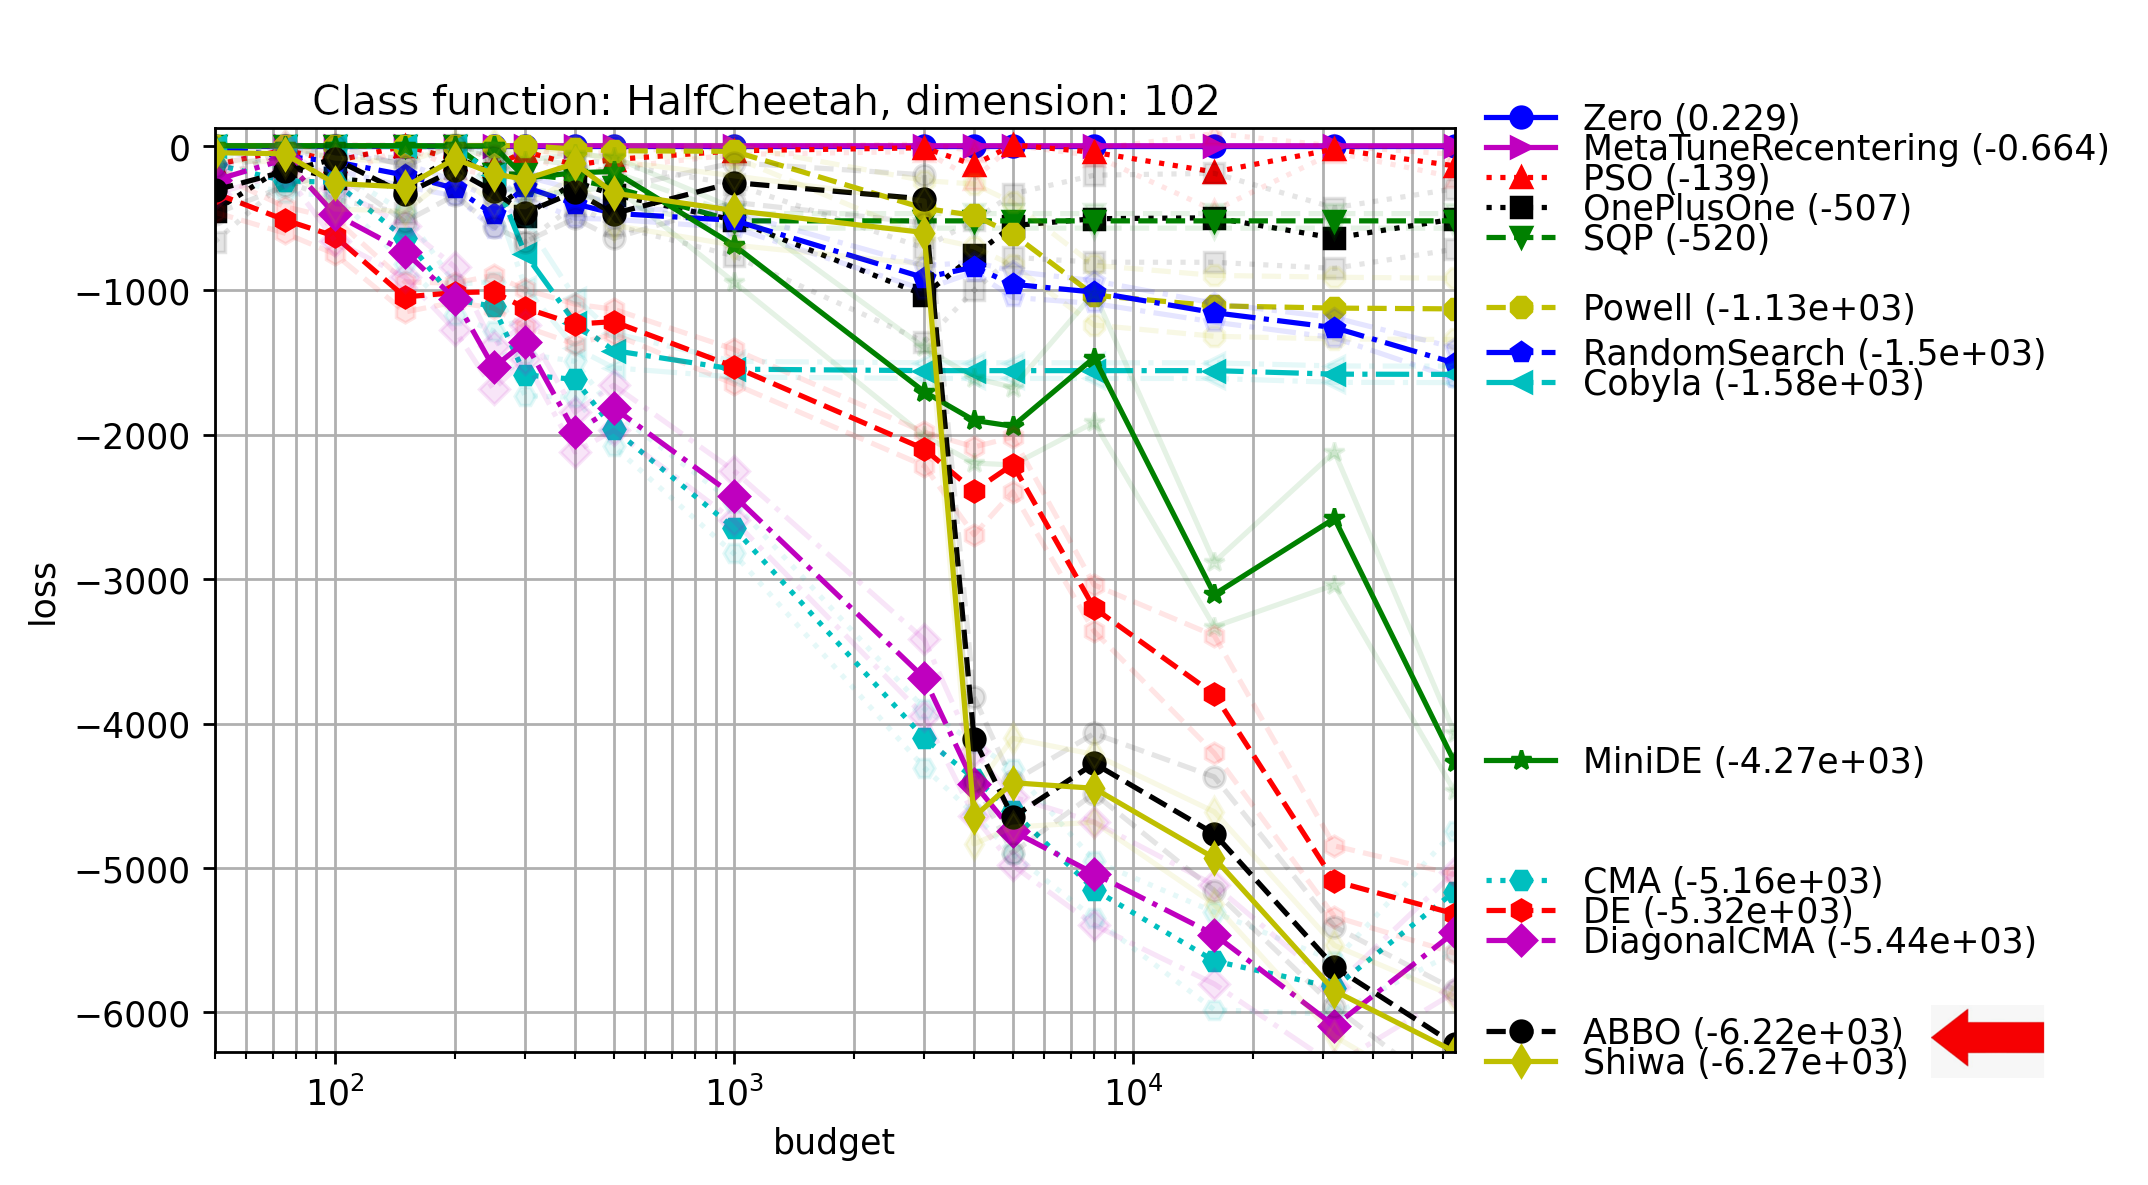
\includegraphics[width=.48\textwidth]{sections/appendix/h220benchmarks/benchmark/control_problem/xpresults_dimension102,function_classHalfCheetah,parametrizationsigma=0.1_edited.png}
    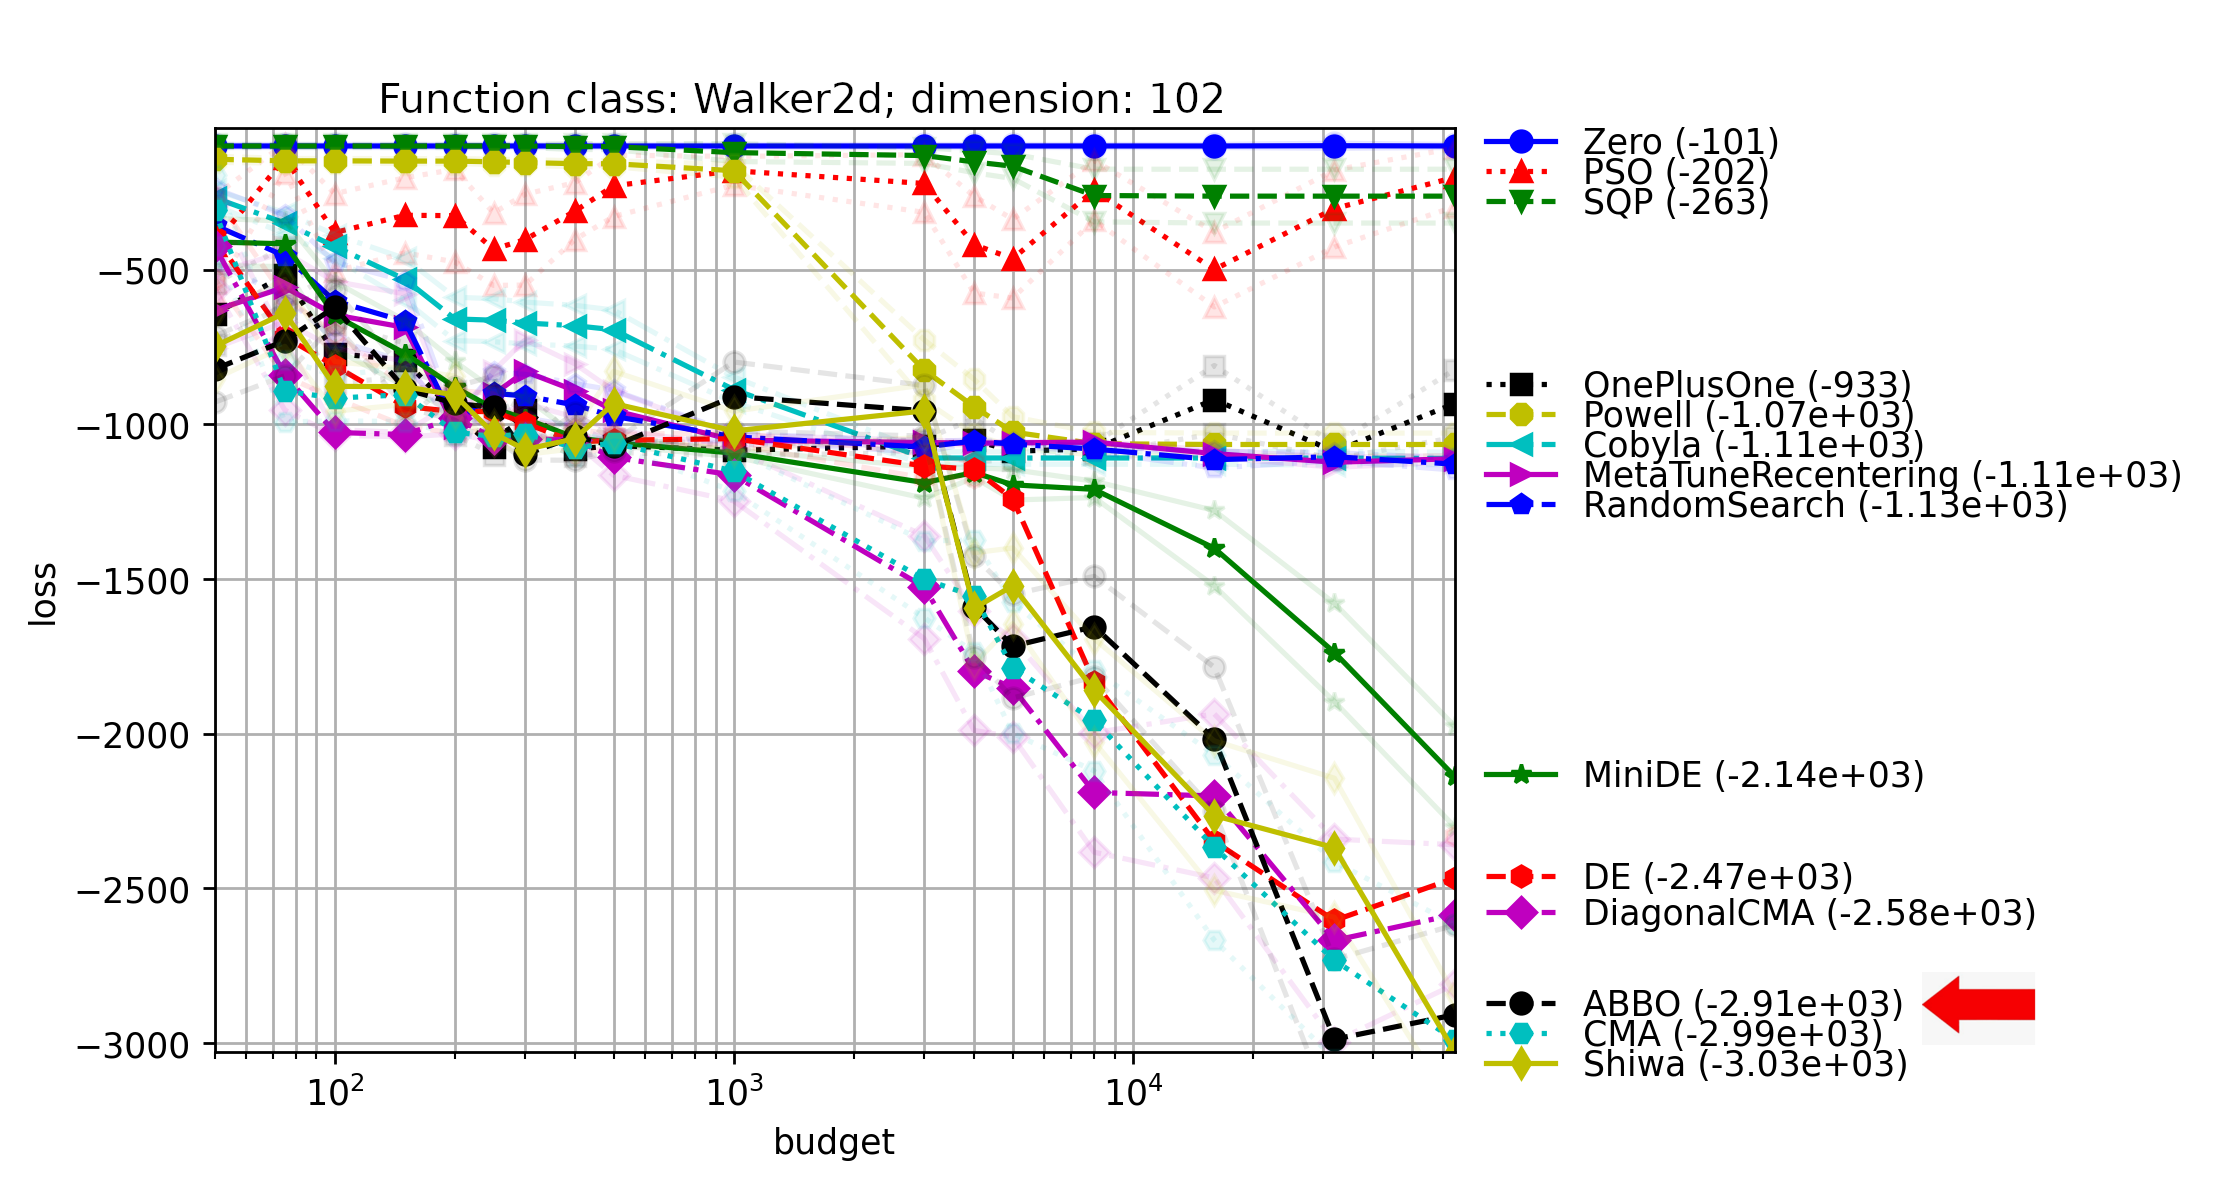
\includegraphics[width=.48\textwidth]{sections/appendix/h220benchmarks/benchmark/control_problem/xpresults_dimension102,function_classWalker2d,parametrizationsigma=0.1_edited.png}\\
    %\twocaptions[Half-Cheetah (dim 102)]{Walker-2d (dim 102)}
        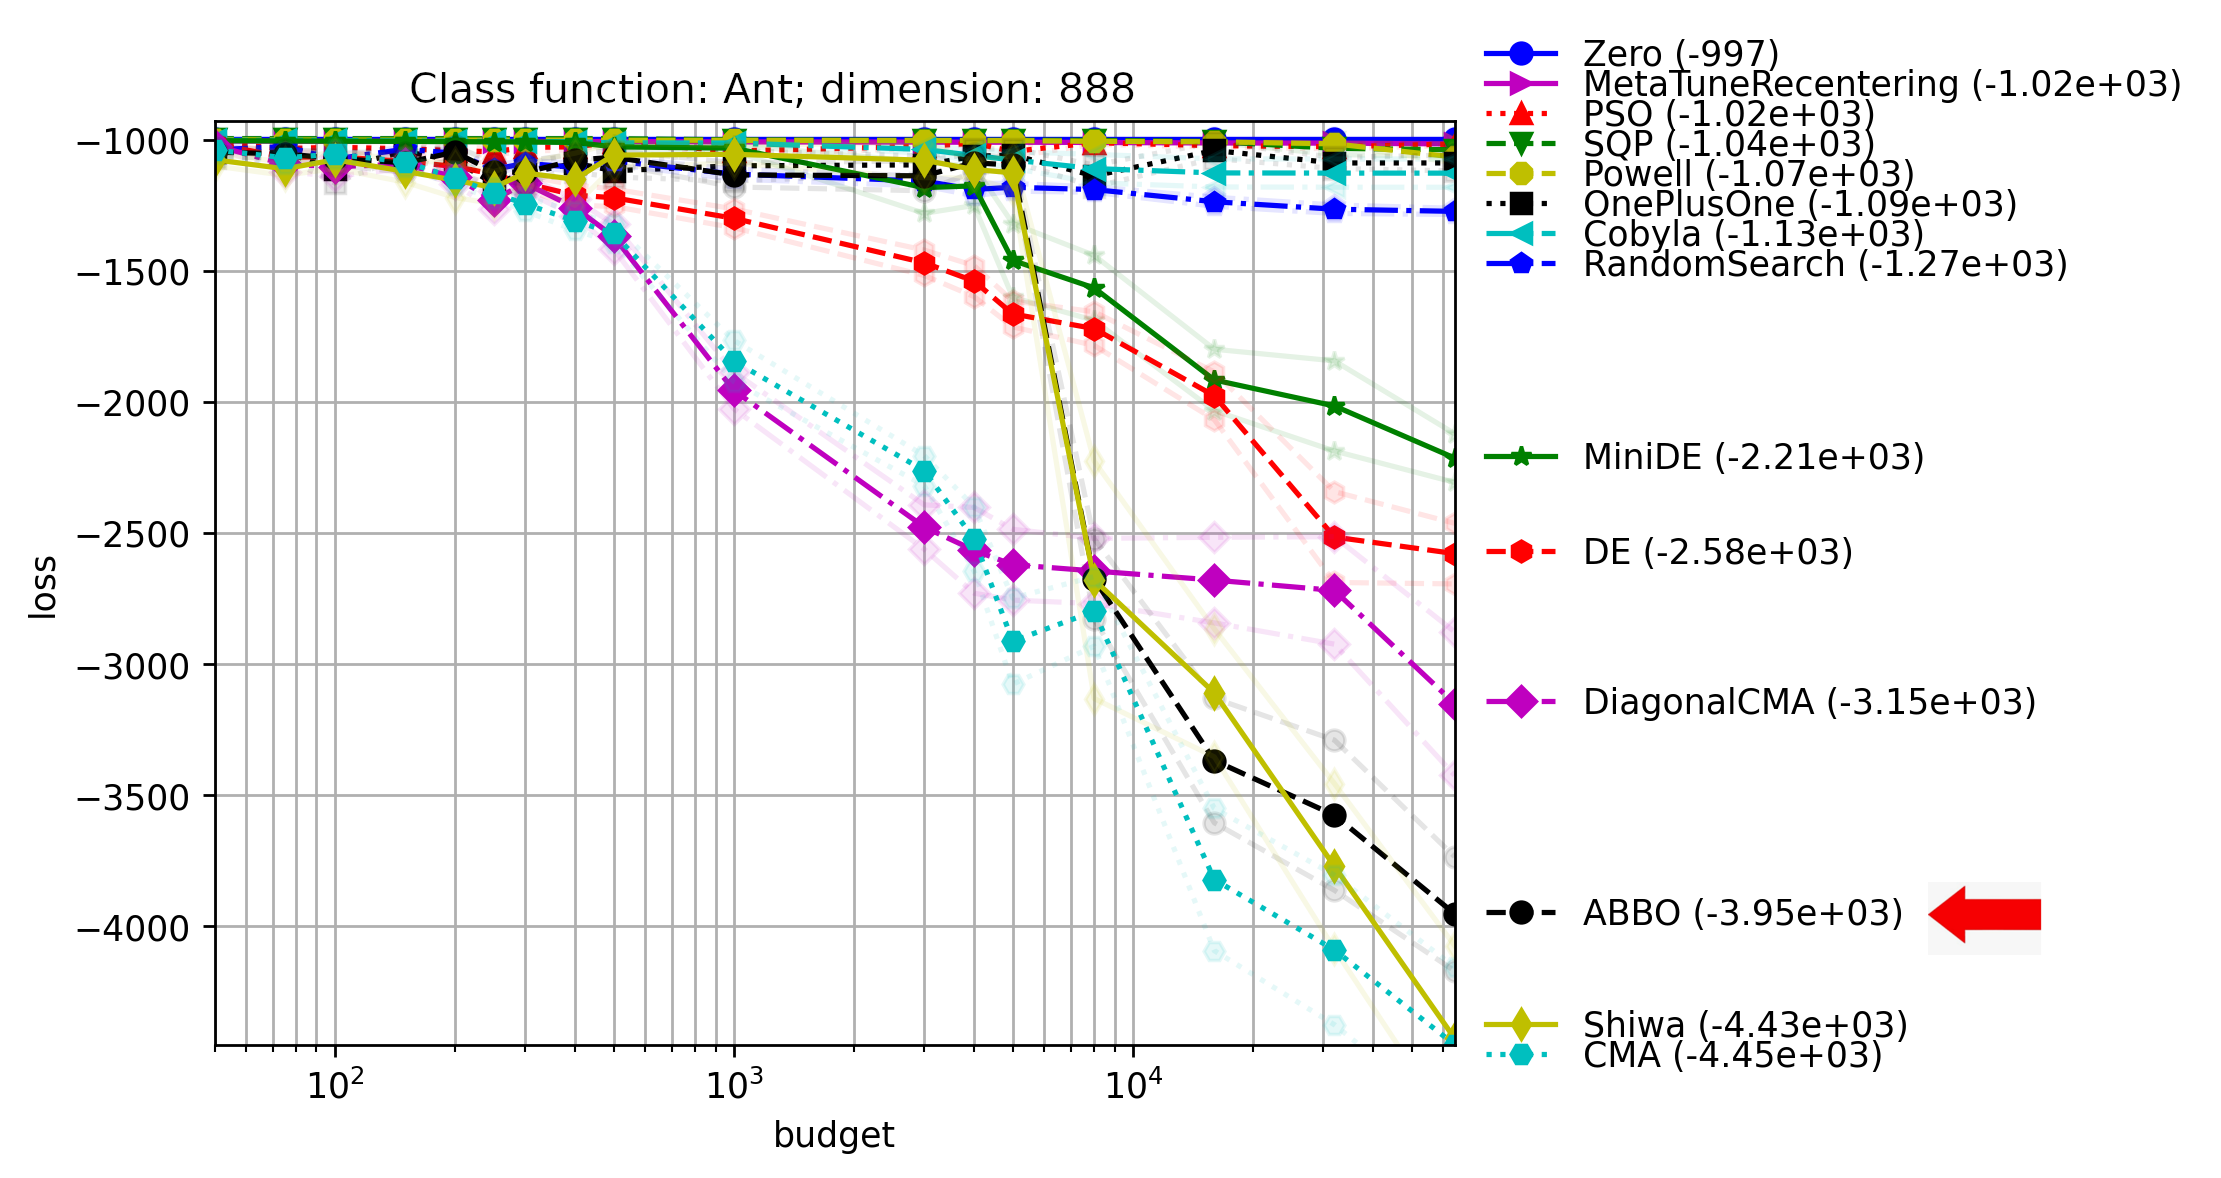
\includegraphics[width=.48\textwidth]{sections/appendix/h220benchmarks/benchmark/control_problem/xpresults_dimension888,function_classAnt,parametrizationsigma=0.01_edited.png}
    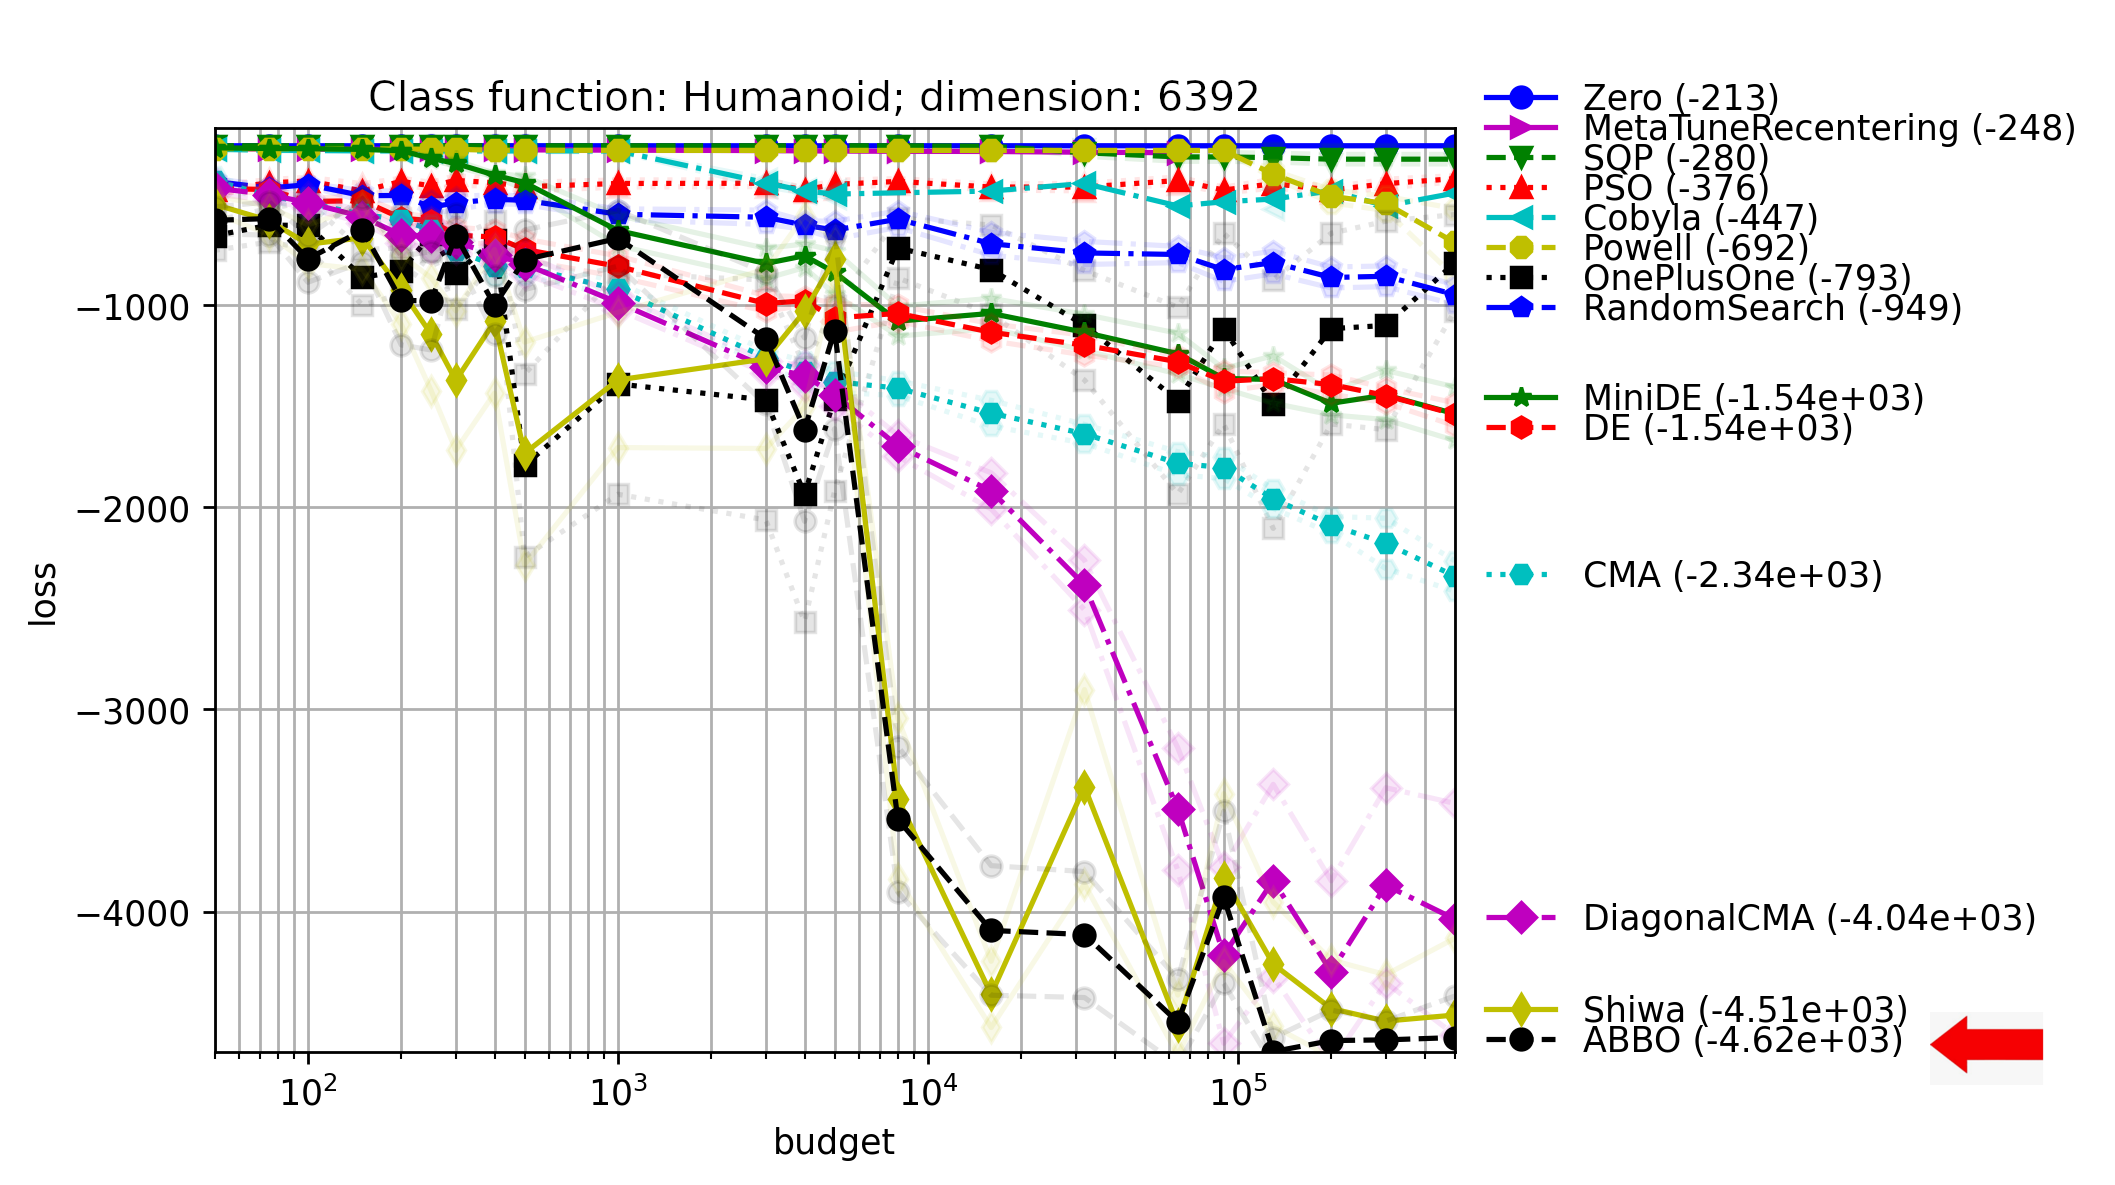
\includegraphics[width=.48\textwidth]{sections/appendix/h220benchmarks/benchmark/control_problem/xpresults_dimension6392,function_classHumanoid,parametrizationsigma=0.001_edited.png}\\
    %\twocaptions[Ant (dim 888)]{Humanoid (dim 6392)}
	\caption{Results on the MuJoCo testbeds. Dashed lines show the standard deviation. Compared to the state of the art in~\cite{lamcts}, with an algorithm adapted manually for the different tasks, we get overall better results for Humanoid, Ant, and Walker. We get worse results for Swimmer (could match if we had modified our code for the three easier tasks as done in~\cite{lamcts}), similar for Hopper and Cheetah: we reach the target for 5 of the 6 problems (see main text). Runs of Shiwa correspond to the improvement of Shiwa due to chaining, as explained in Sec.~\ref{ngopt}.}
    \label{figMuJoCobis}
\end{figure*}

{\textbf{Additional new artificial and real-world functions:}}\label{b6}
\textbf{LSGO}~\cite{lsgo} combines various functions into an aggregated testbed including composite highly multimodal functions. Correctly decomposing the problem is essential.
Various implementations of LSGO exist; in particular, {the Octave and C++ versions do not match exactly for F3/F6/F10. We match the C++ version, which is the one used in~\cite{lsgo}. For F7, there is a difference between the code and the paper and we match the code rather than the paper.} 
Following~\cite{lsgo}, our implementation comprises functions with subcomponents (i.e., groups of decision variables) having non-uniform sizes and non-uniform, even conflicting, contributions to the objective function. 
We also present experimental results on \textbf{SequentialFastgames} from the Nevergrad benchmarks, and three newly introduced benchmarks, namely \textbf{Rocket}, \textbf{Simple TSP} (a set of traveling salesman problems, {where a vector $x\in \RR^d$ is converted into a permutation $\sigma$ by letting $\sigma(i)$ be the index of the $i$-th largest element in $x$ (ties broken at random)}), and \textbf{power systems} (unit commitment problems~\cite{unitcommitment}). Experimental results are presented in Figs.~\ref{figaddrw},~\ref{figaddrwbis}, and~\ref{figaddrwbisbis}, respectively. They show that \ngoptq{} performs well on new benchmarks, never used for its design nor for that of the low-level heuristics used inside \ngoptq{}. 

 \begin{table*}
	    \caption{{ Results on MuJoCo for a linear policy in the black-box setting from~\cite{lamcts} and references therein. We compare various published results to results from \ngoptq{}.} \textcolor{black}{Two last {columns} = average reward for the maximum budget tested in~\cite{lamcts}, namely 1k, 4k, 4k, 40k, 30k, 40k, respectively.} ``ioa'' = iterations on average for reaching the target.  ``iter'' = iterations for target reached for median run. ``*'' refers to problems for which the target was not reached by~\cite{lamcts}: then BR means ``best result in 10 runs''. \ngoptq{} reaches the target for Humanoid and Ant whereas previous (black-box) papers did not; we get nearly the same ioa for Hopper and HalfCheetah (Nevergrad computed the expected value instead of computing the ioa, so we cannot compare exactly; see  Fig.~\ref{figMuJoCobis} for curves). \ngoptq{} is slower than LA-MCTS on Swimmer. Note that we keep the same method for all benchmarks whereas LA-MCTS modified the algorithm for 3 rows. On HDMULTIMODAL, \ngoptq{} performs better than LA-MCTS, as  detailed in the text, and as confirmed in~\cite{lamcts}, which acknowledges the poor results of LA-MCTS for high-dimensional Ackley and Rosenbrock.}
    \label{lamctsnumbers}
        \centering
        \setlength{\tabcolsep}{1pt}
       \scriptsize
\begin{tabular}{|l|c|c|c|c|c|}
		\hline
	%\textbf{Problem} & \textbf{Target (ioa)} & \textbf{SOTA w/o grad (ioa)} & \textbf{SOTA w grad} &  \textbf{\ngoptq{}} \\
        %\textbf{Problem} & \textbf{Target (ioa)} & \textbf{SOTA w/o grad (ioa)} & \textbf{SOTA w grad (ioa)} &  \textbf{\ngoptq{} result (ioa)} \\
        \textbf{Task} & \textbf{Target} & \textbf{LA-MCTS results} &  \textbf{\ngoptq{} result} &\textbf{\textcolor{black}{LA-MCTS avg reward}}&\textbf{\textcolor{black}{\ngoptq{} avg reward}}\\ 
%                & \cite{lamcts} & with grad &  \\
%		&  & & \\
                \hline 		  \hline
        Swimmer-v2 & 325 &  132 \textcolor{black}{ioa} &     around $ 450$ iter & {{358}} & {\textbf{365}} \\   \hline
        Hopper-v2 & 3120 &  2897 \textcolor{black}{ioa}  &    around $ 3\,000$ iter & {\textbf{3292}} & 1787 \\ \hline
        HalfCheetah-v2 &  3430 &  3877 \textcolor{black}{ioa}  &  around $ 4\,000$ iter & {{3227}} & {\textbf{4730}} \\ \hline
Walker2d-v2*  & 4390 &  BR: 3314 (not reached) &  BR: \textbf{4398}, budget $<64\,000$  & 2769 & {\textbf{2949}} \\  \hline
        Ant-v2*  & 3580 &  BR: 2791 (not reached) &    BR: \textbf{5325}, budget $<32\,000$  & 2511 & {\textbf{3532}} \\ \hline
        Humanoid-v2* & 6\,000 &  BR: 3384 (not reached)&   BR (budget 5\,00000): {\textbf{4870}}  & 2511 & {\textbf{4620}}\\
        \hline
        \end{tabular}
    \end{table*}
    
\begin{figure*}[t]
\centering
\vspace{-0.2cm}
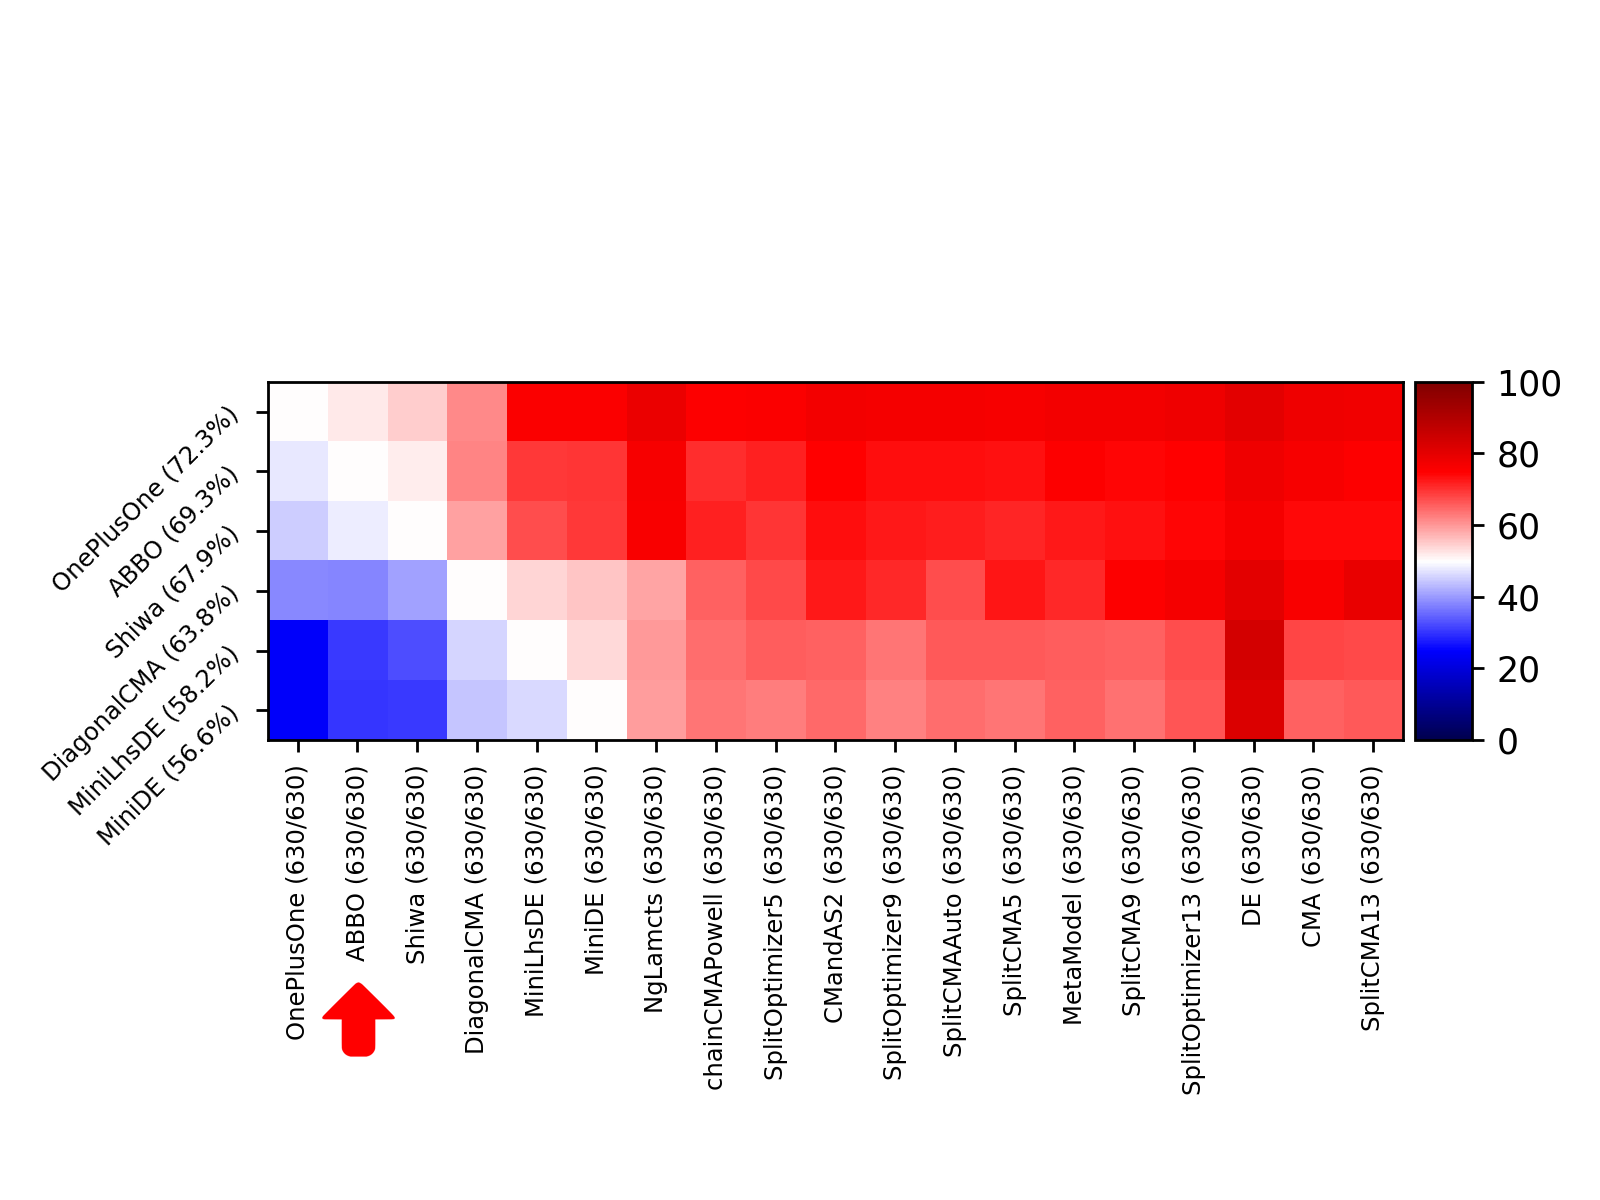
\includegraphics[trim={0 10 0 100},clip,width=.48\linewidth]{sections/appendix/h220benchmarks/benchmark/fa_yahdbbob.png}
    %\onecaption{High-dimensional (HD)}\\
    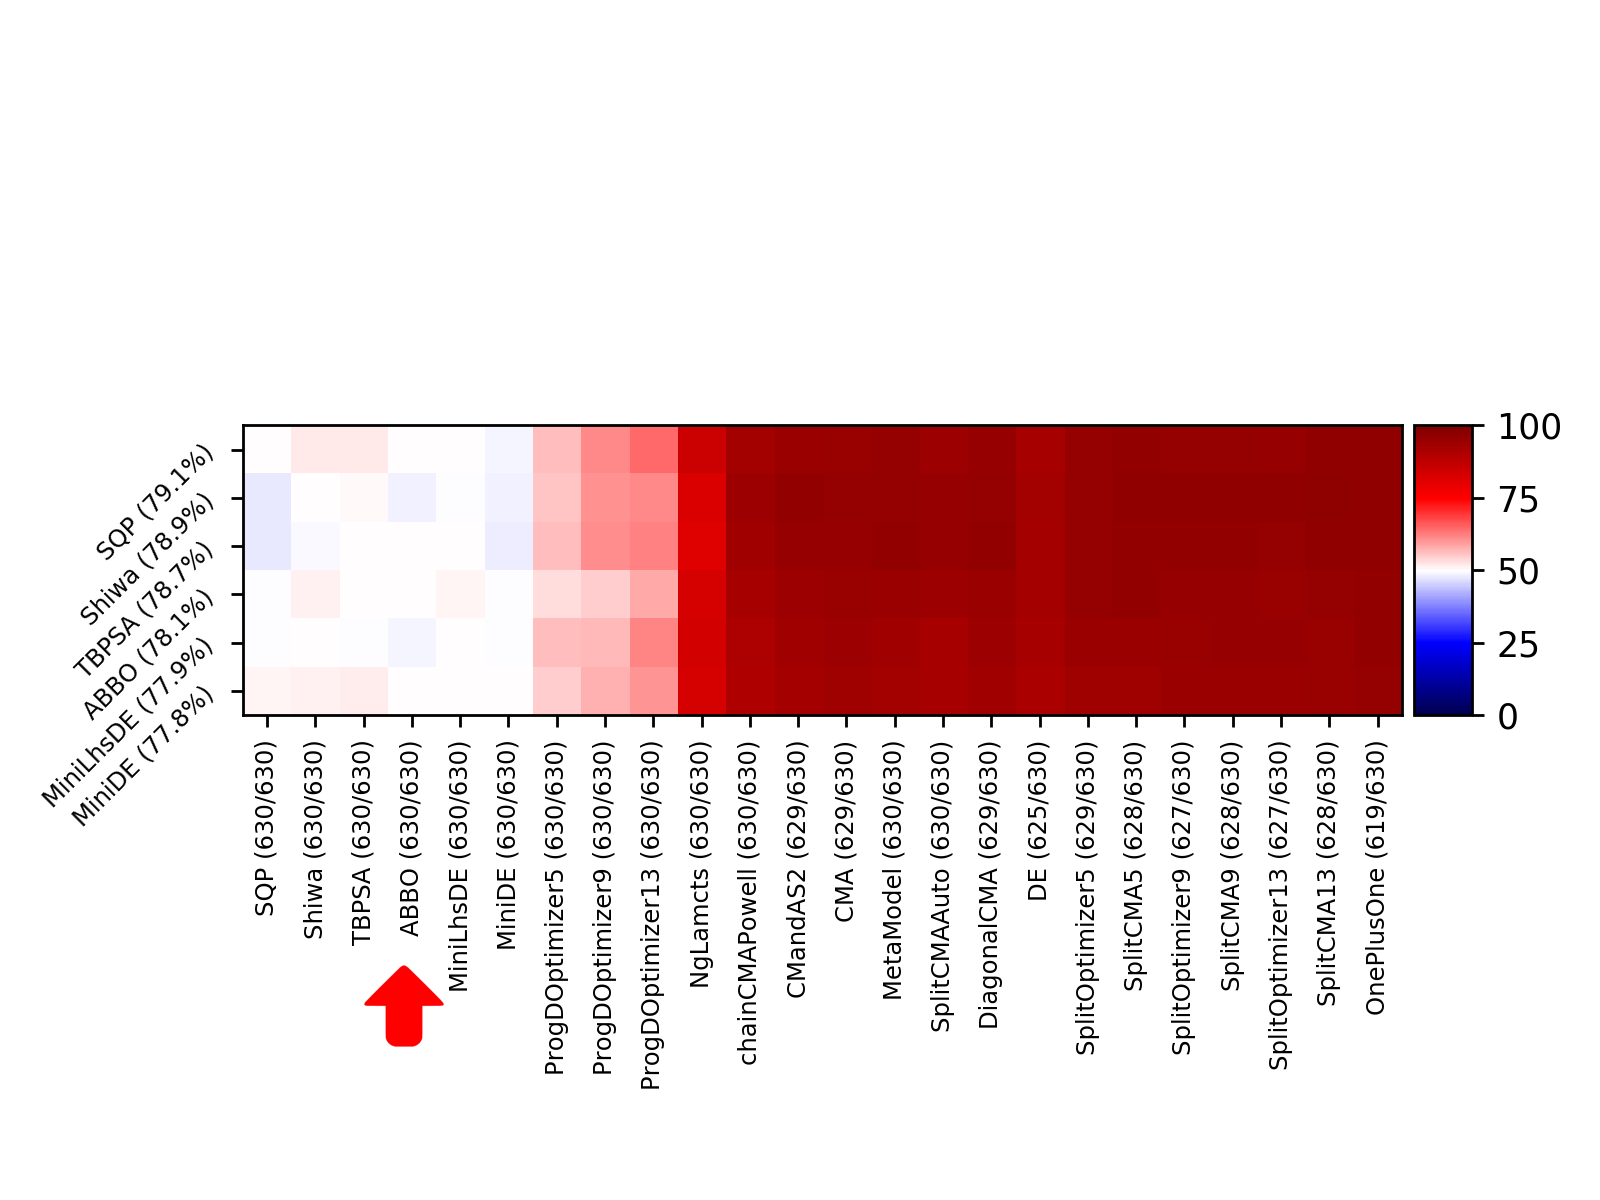
\includegraphics[trim={0 0 0 100},clip,width=.48\linewidth]{sections/appendix/h220benchmarks/benchmark/fa_yahdnoisybbob.png}
    %\onecaption{Noisy HD}\\
     %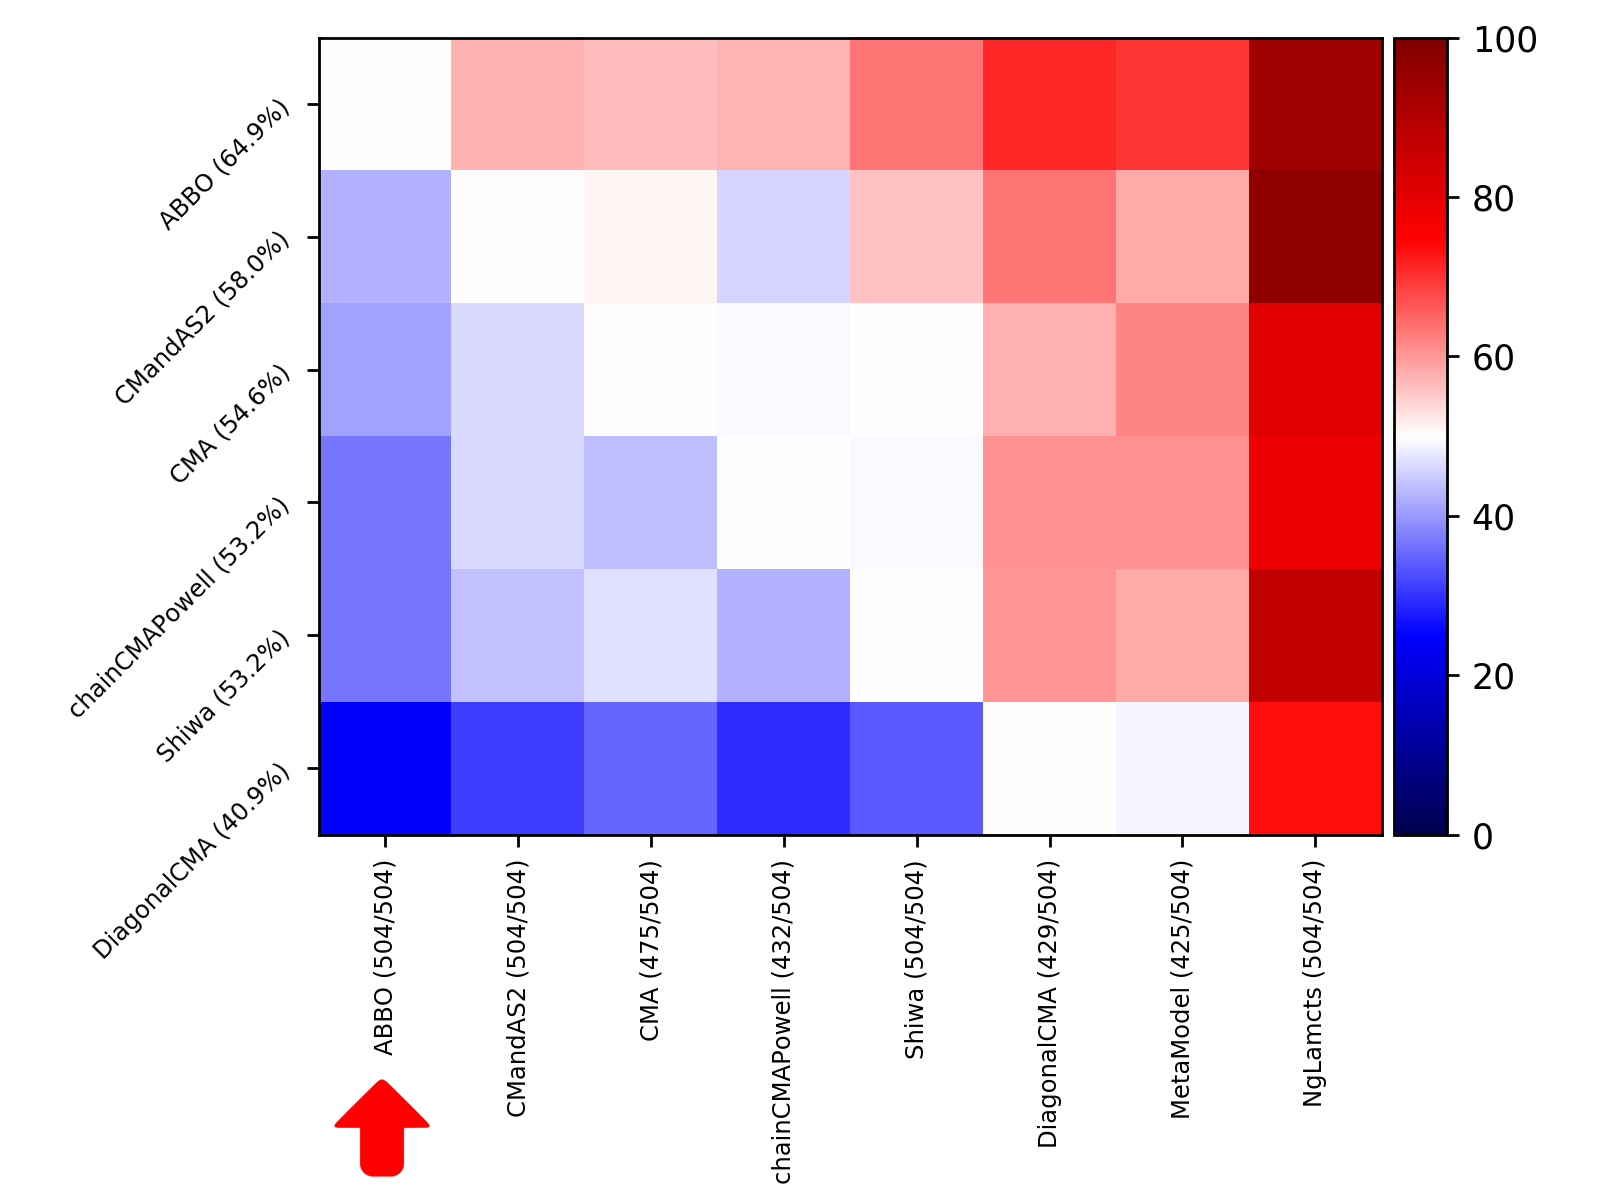
\includegraphics[trim={0 0 0 9},clip,width=.45\linewidth]{benchmark/fa_yabigbbob.png}\\
    %%\onecaption{Big budget}\\
%    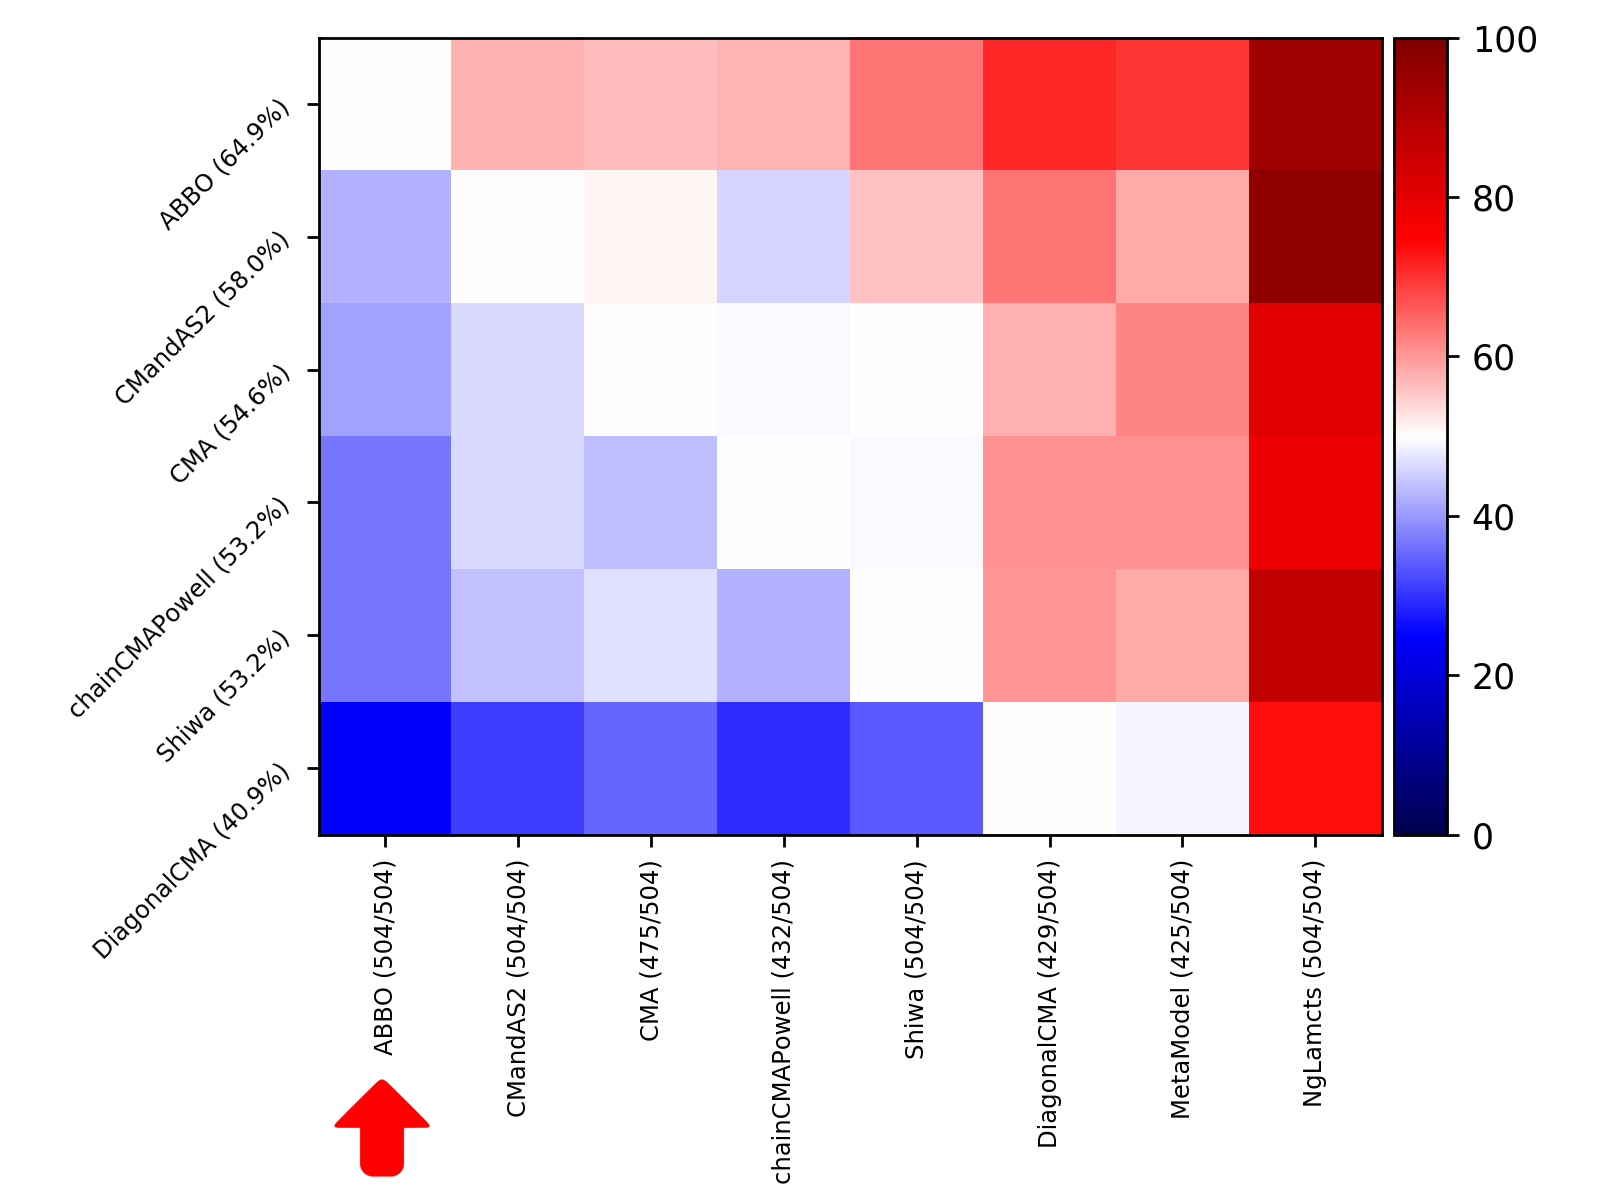
\includegraphics[width=.4\linewidth]{benchmark/fa_yabigbbob.png}
%        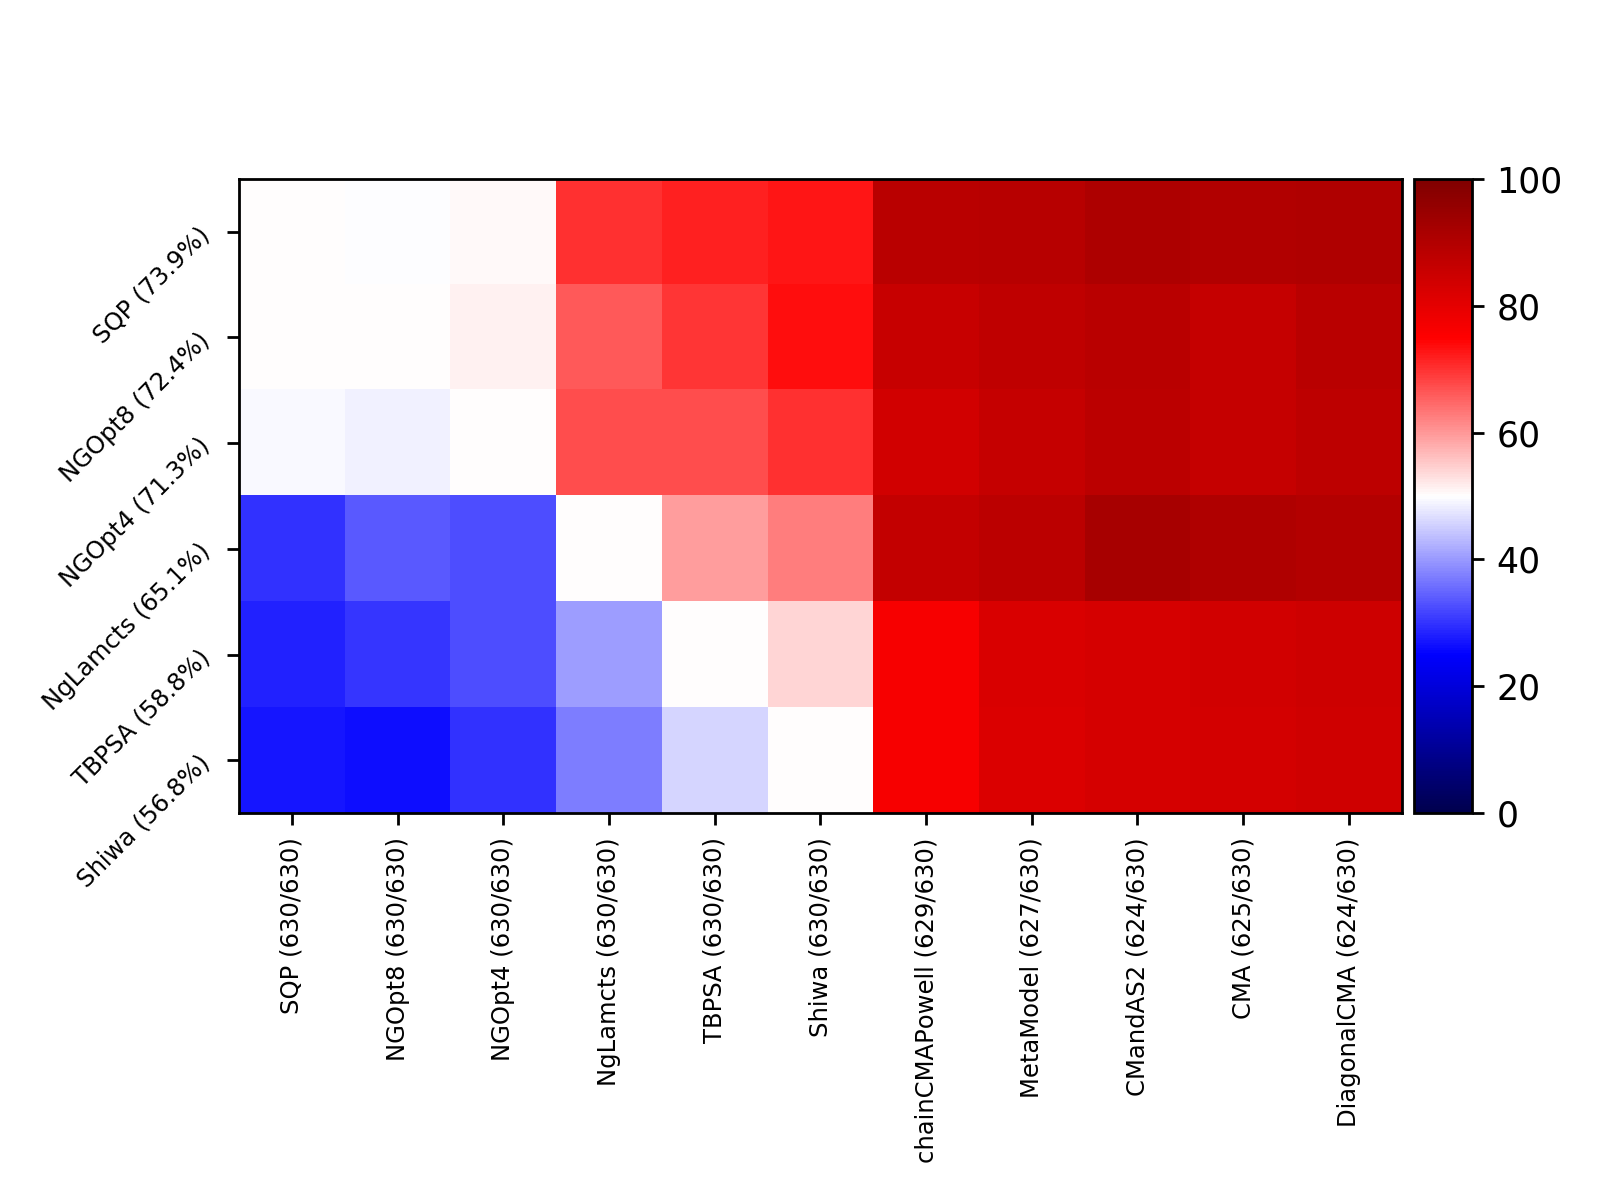
\includegraphics[width=.4\linewidth]{benchmark/fa_yanoisybbob.png}
%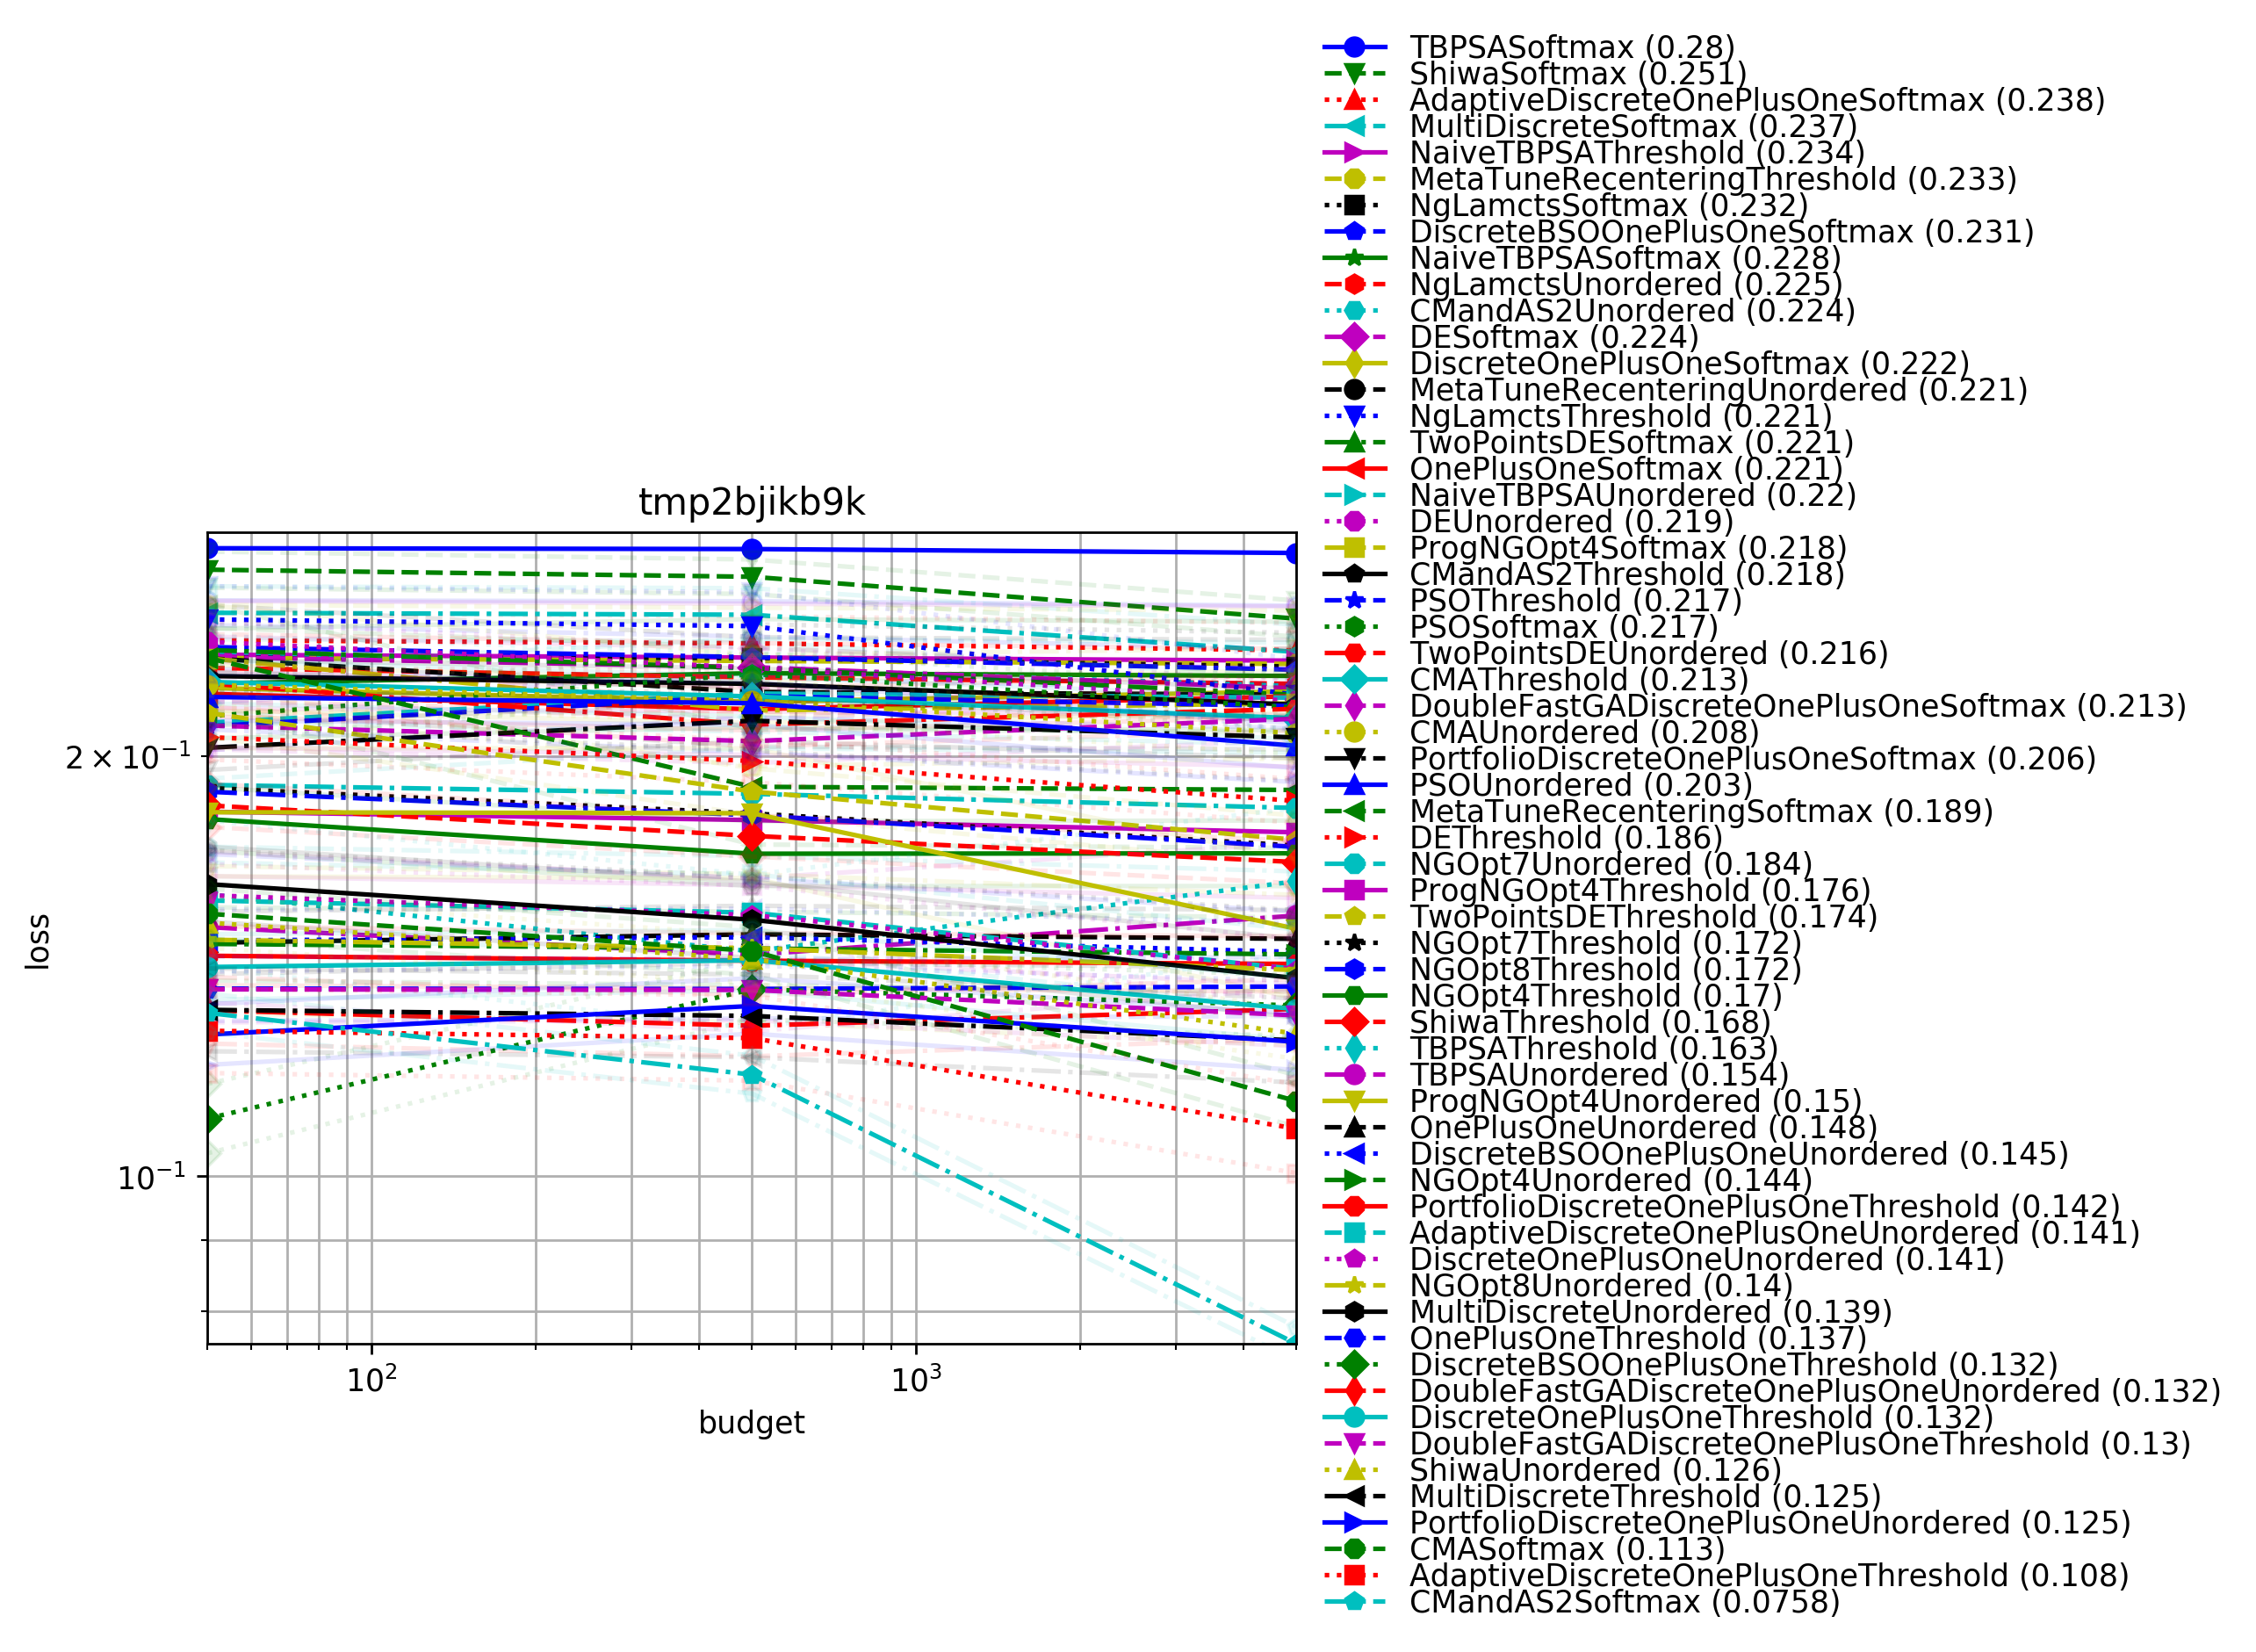
\includegraphics[width=.4\linewidth]{benchmark/xp_instrum_discrete.png}
%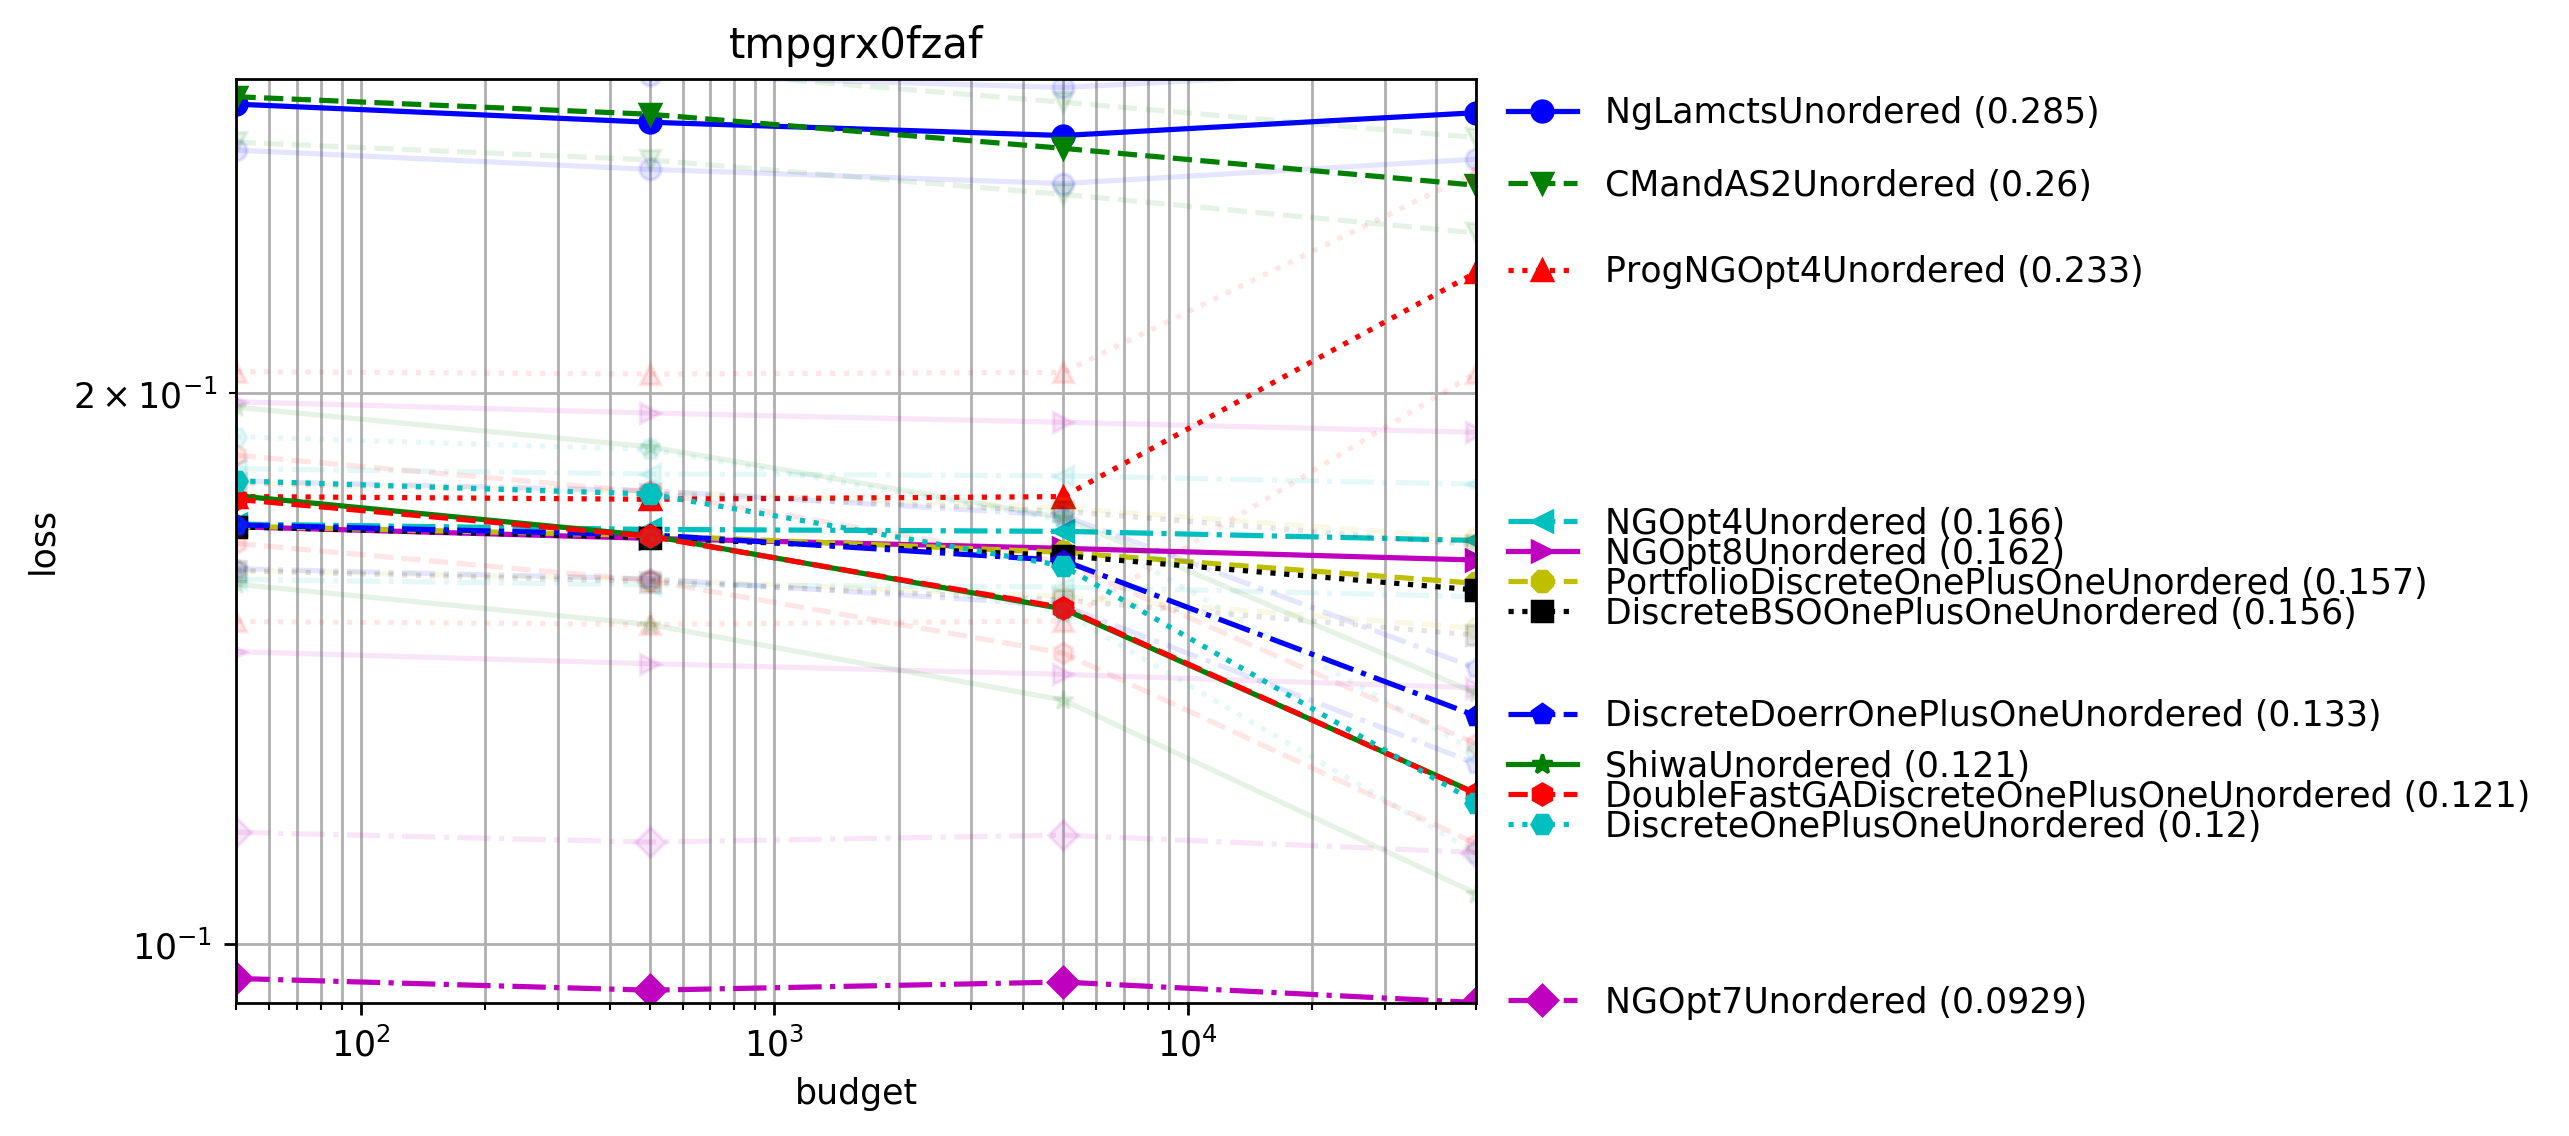
\includegraphics[width=.4\linewidth]{benchmark/xp_sequential_instrum_discrete.png}\\
%%\twocaptions[InstrumDiscrete]{SequentialInstrumDiscrete}
	\caption{YAHDBBOB (dimension $\geq 50$) and YANOISYHDBBOB (noisy + dimension $ \geq 50$)  heatmaps.}
    \label{bbobfigbis}
\end{figure*}
\begin{figure*}[ht]
    \centering
    \includegraphics[trim={0 0 0 150},clip,width=0.49\linewidth]{sections/appendix/h220benchmarks/benchmark/xp_alldes.png}
    \includegraphics[trim={0 0 0 45},clip,width=0.49\linewidth]{sections/appendix/h220benchmarks/benchmark/xp_hdbo4d.png}
	%\onecaption{HDBO ($d\in\{20,2\,000\}$)}\\
%    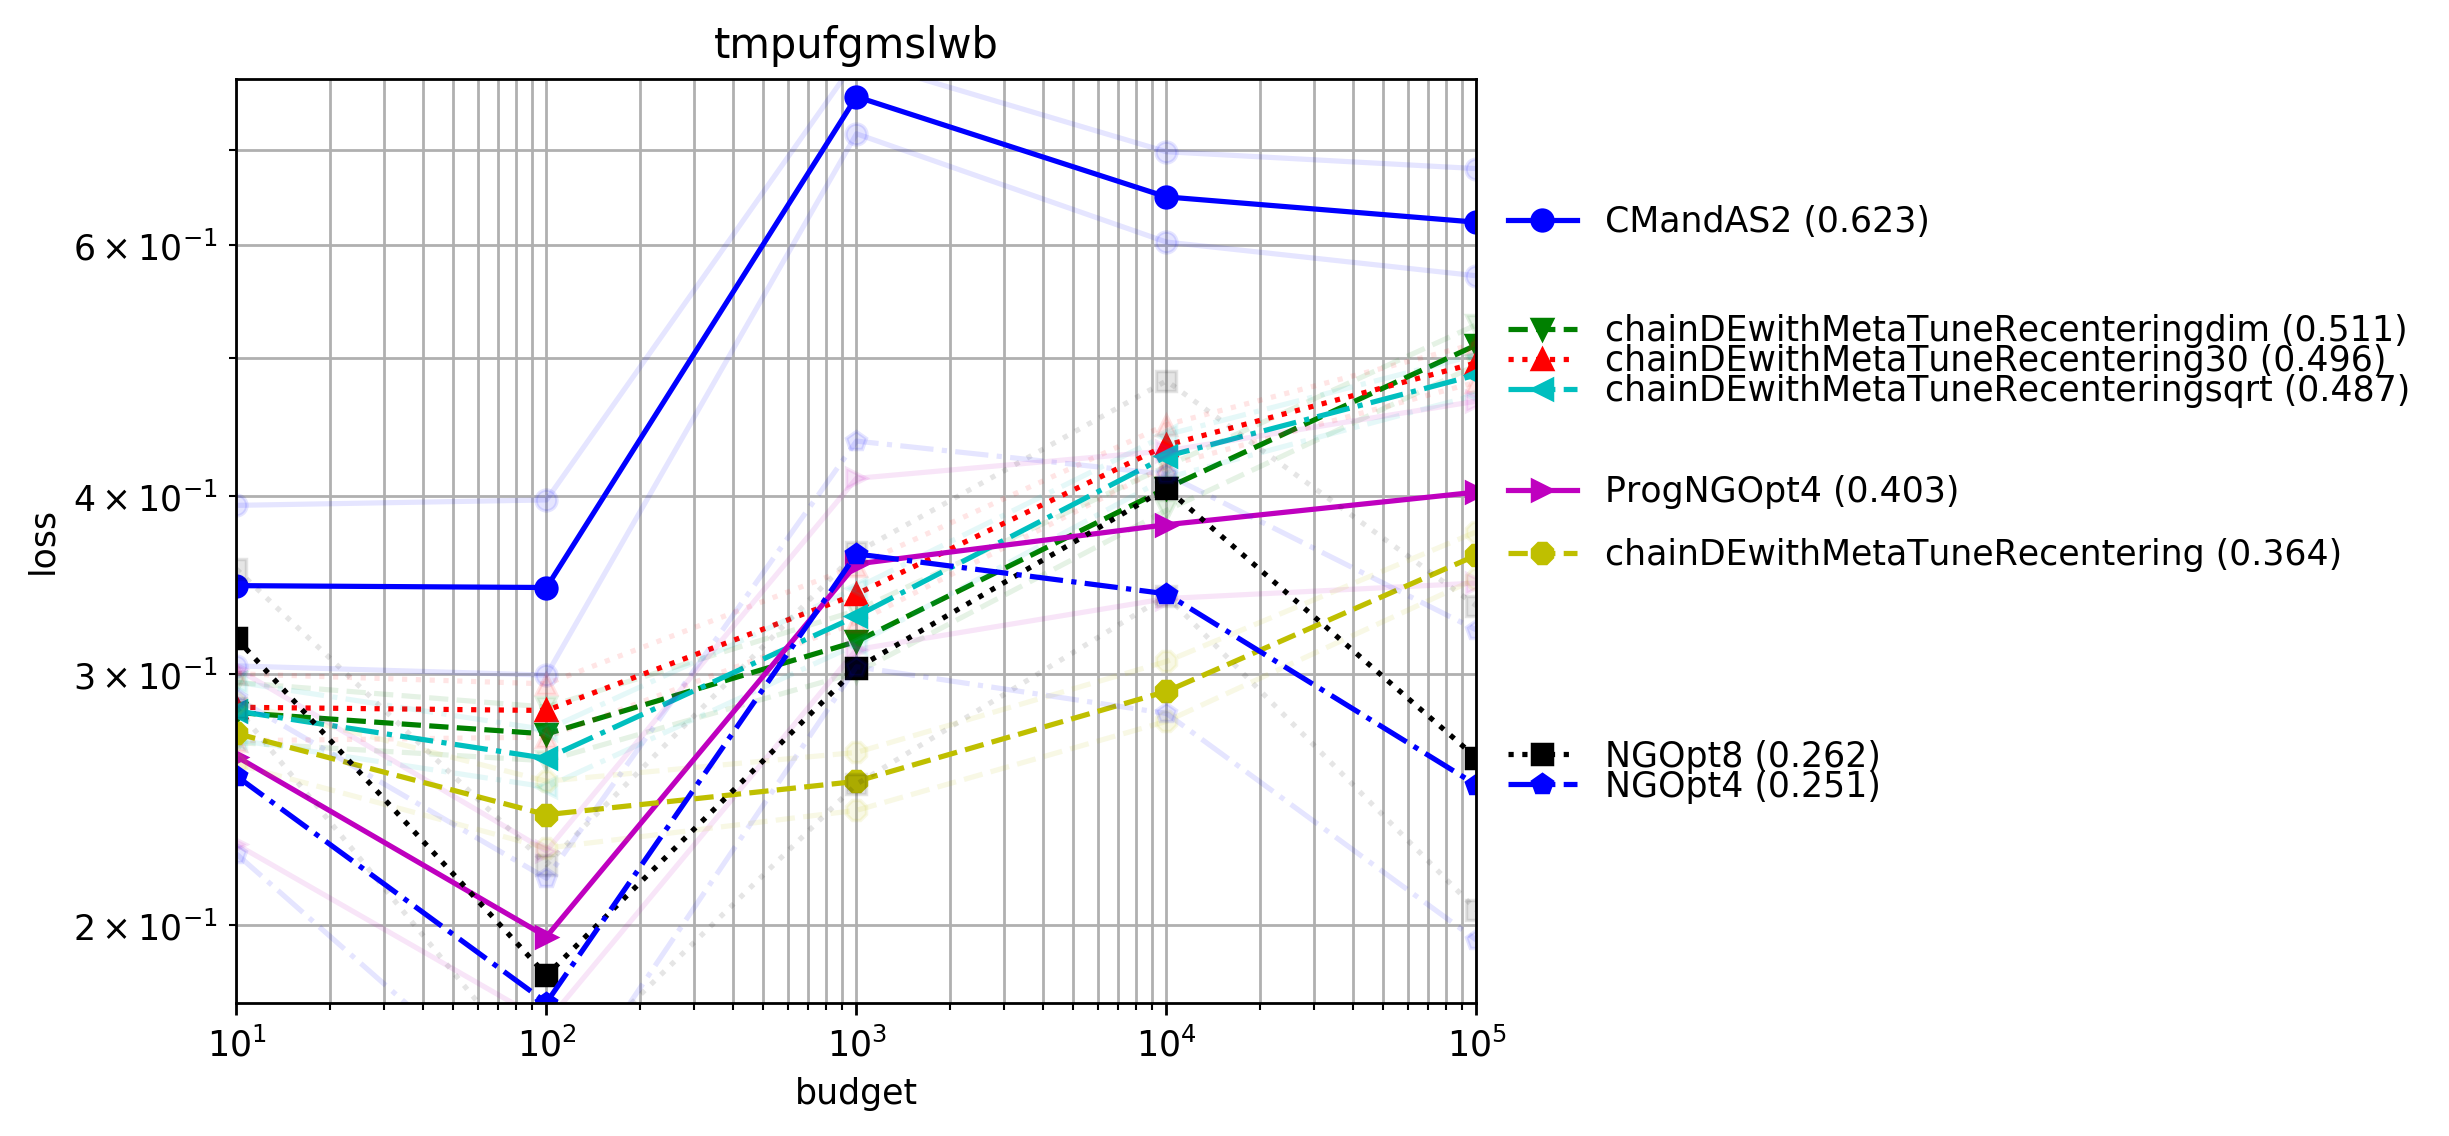
\includegraphics[width=.4\linewidth]{benchmark/xp_paraalldes.png}\\   
%    %\twocaptions[AllDEs]{Para-AllDEs}
%    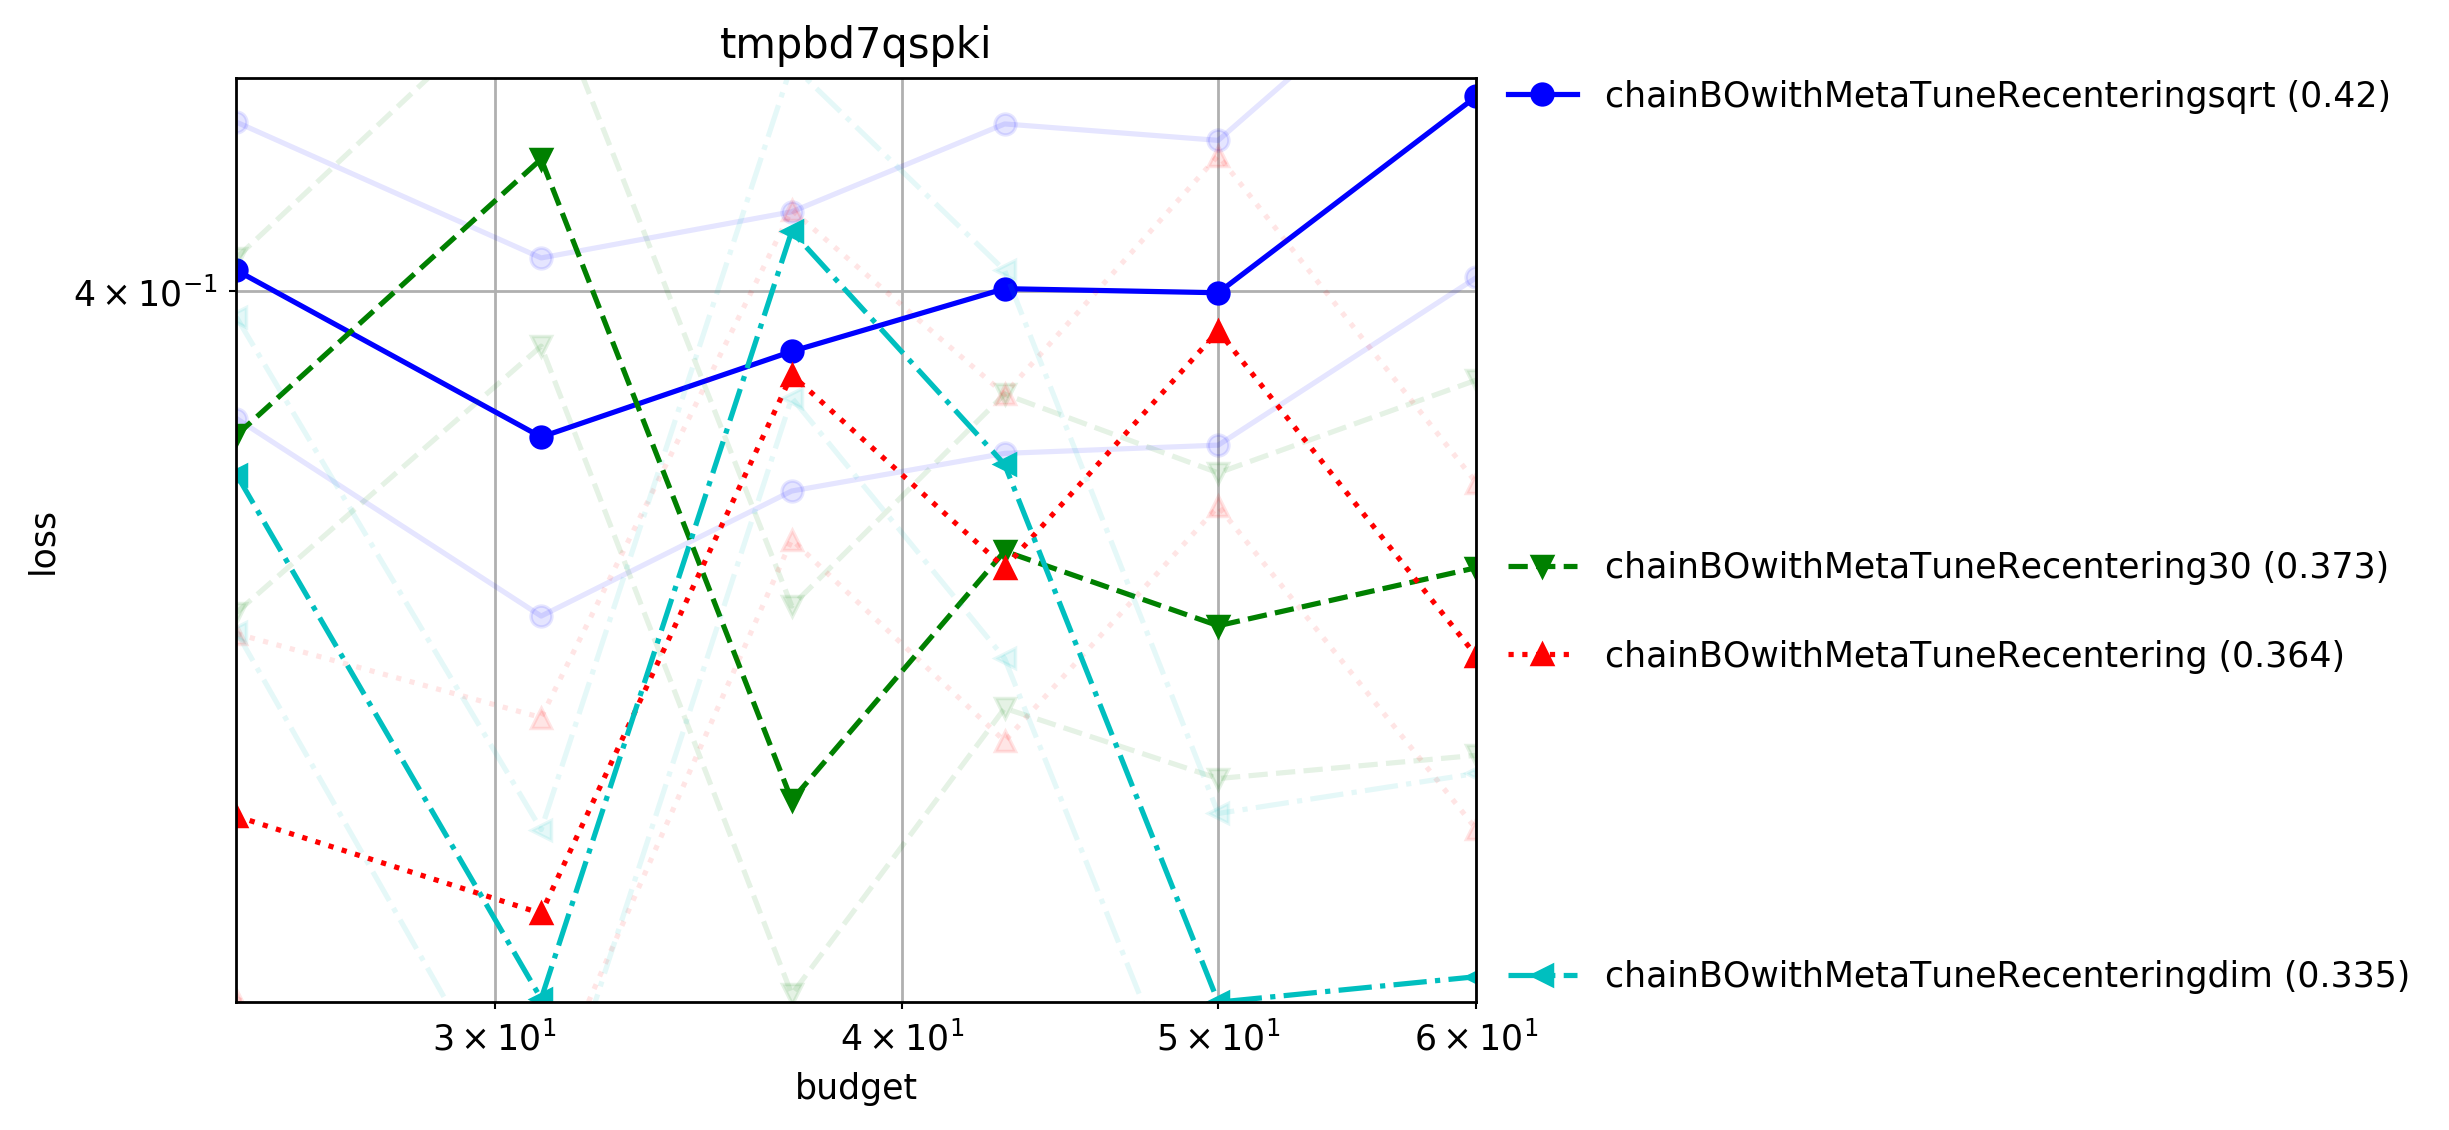
\includegraphics[width=.4\linewidth]{benchmark/xp_parahdbo4d.png}\\
%    %\twocaptions[HDBO]{Para-HDBO}
    \caption{\ngoptq{} vs specific families of optimization algorithms {(DE on the left in dimension 5, 20 and 100; and BO in dimension 20 on the right) on Cigar, Hm, Ellipsoid, Sphere functions.} Not all run algorithms are mentioned, for short. {Bayesian optimization {(Nevergrad uses~\cite{BOpython})}, often exploring boundaries first, is outperformed in high dimension}~\cite{lamcts}.}
    \label{specif}
\end{figure*}

\begin{figure*}[t!]
\centering
\includegraphics[trim={0 0 0 54},clip,width=.49\linewidth]{sections/appendix/h220benchmarks/benchmark/xp_paramultimodal.png}
\includegraphics[trim={0 0 0 21},clip,width=.49\linewidth]{sections/appendix/h220benchmarks/benchmark/xp_realworld.png}
%\includegraphics[width=.4\linewidth]{benchmark/fa_far_optimum_es.png}\\
%\onecaption{PARAMULTIMODAL}\\
%\vspace{0.5cm}
%\includegraphics[width=.4\linewidth]{benchmark/fa_realworld.png}\\ 
%\onecaption{Realworld}

	\caption{Left: experiments for the parallel multimodal setting PARAMULTIMODAL. Budget up to 100\,000, parallelism 1\,000, Ackley+Rosenbrock+DeceptiveMultimodal+Griewank+Lunacek+Hm. Right: Realworld benchmark from Nevergrad: games, Sammon mappings, clustering, small traveling salesman instance, small power systems.}\label{figrw}
\end{figure*}

\begin{figure*}[t]
    \centering
%\includegraphics[width=.4\linewidth]{benchmark/fa_pyomo.png}\\ 
\includegraphics[trim={0 0 0 21 },clip,width=.48\linewidth]{sections/appendix/h220benchmarks/benchmark/xp_rocket.png}
%\includegraphics[width=.4\linewidth]{benchmark/fa_rocket.png}\\ 
%%\onecaption{Rocket}\\
%\onecaption{Rocket}\\
%\vspace{0.5cm}
\includegraphics[trim={0 0 0 21},clip,width=.48\linewidth]{sections/appendix/h220benchmarks/benchmark/xp_simpletsp.png}
%\includegraphics[width=.4\linewidth]{benchmark/fa_powersystems.png}\\ 
%\onecaption{SimpleTSP}

	\caption{{Additional  problems (1): on left, Rocket (26 continuous variables, budget up to 1600, sequential or parallelism 30) and on right, SimpleTSP (10 to 1\,000 decision variables).}}
	\label{figaddrwbis}
\end{figure*}

\begin{figure*}[t]
    \centering
\includegraphics[trim={0 0 0 125},clip,width=.48\linewidth]{sections/appendix/h220benchmarks/benchmark/xp_powersystems.png}
%\includegraphics[width=.4\linewidth]{benchmark/fa_powersystems.png}\\ 
%\onecaption{PowerSystems}\\
\vspace{0.5cm}
%%\onecaption{Power System}\\
\includegraphics[trim={0 0 0 10},clip,width=0.48\linewidth]{sections/appendix/h220benchmarks/benchmark/xp_lsgo.png}
%\includegraphics[width=.4\linewidth]{benchmark/fa_photonics.png}\\ 
%	%\onecaption{Photonics}\\
%\onecaption{Lsgo (15 functions)}
\caption{{Additional problems (2): on left, PowerSystems (1806 to 9646 neural decision variables) and  on right, LSGO (mix of partially separable, overlapping, shifted cases as in~\cite{lsgo}).}} 
	\label{figaddrwbisbis}

\end{figure*}

{\textbf{MuJoCo:}}\label{MuJoCo}\label{b7}
% TODO Add ref to ARS paper: https://arxiv.org/pdf/1803.07055.pdf
%{choice for sigmas: 0.1 till dim 102, then 0.01 for 888 and 0.001 for 6392}
Some articles~\cite{lmrs,lamcts} studied the MuJoCo testbeds~\cite{mujoco} in the black-box setting. MuJoCo tasks correspond to control problems. Defined in~\cite{lamcts,ars}, the objective is to learn a linear mapping from states to actions. {
It turned out that the scaling of the variables is critical~\cite{ars}: following the recommendation from~\cite{ppsnrescaling} to sample close to zero in the high dimensional setting, we chose to initialize all the variables of the problem with a variance decaying with the dimension, for all methods run in Fig.~\ref{figMuJoCobis}. We remark that \ngoptq{} and Shiwa perform well, even when compared to gradient-based methods, while having the advantage of being applicable to settings in which gradients are not available. In comparison to gradient-based methods, black-box methods do not require computation of the gradient, and hence, save computational time.}

We use the same experimental setup as~\cite{lamcts} (linear policy, offline whitening of states).	We get better results than LA-MCTS, in a setting without using any expensive surrogate model (Tab.~\ref{lamctsnumbers}). Our runs with CMA-ES and Shiwa are better than those in~\cite{lamcts}. We acknowledge that LMRS~\cite{lmrs} outperforms our method on all MuJoCo tasks, using a deep network as a surrogate model: however, we point out that a part of their code is not open sourced, making the experiments not reproducible. In addition, when rerunning their repository without the closed source part, it solved Half-Cheetah within budget 56k, which is larger than ours. For Humanoid, the target was reached at 768k, which is again larger than our budget. 
The results from \ngoptq{} are comparable to, and are usually better than (for the 3 hardest problems) the results from LA-MCTS, while \ngoptq{} is entirely reproducible. In addition, it runs the same method for all benchmarks and it is not optimized for each task specifically as in~\cite{lmrs,lamcts}. In contrast to \ngoptq{}, LA-MCTS~\cite{lamcts} uses different underlying regression methods and sampling methods depending on the MuJoCo task, and it is not run on other benchmarks except for some of the HDMULTIMODAL ones. On the latter, \ngoptq{} performances are significantly better for Ackley and Rosenbrock in dimension 100 (average results around 100 and $10^{-8}$ after 10k iterations for Rosenbrock and Ackley respectively for \ngoptq{}, vs. 500 and 0.5 in~\cite{lamcts}). From the curves in~\cite{lamcts} and those presented here in this paper, we expect LA-MCTS to perform well with an adapted choice of parametrization and with a low budget, for tasks related to MuJoCo, whereas \ngoptq{} is adapted for wide ranges of tasks and budgets.

{As mentioned at the end of the introduction, videos illustrating the performance of the learnt policies are available at~\cite{zenodo}.}

\def\removedrescaledMuJoCo{
\begin{figure}[t]
    \centering
    \includegraphics[width=.4\textwidth]{sections/appendix/h220benchmarks/benchmark/rescaled_control_problem/xpresults_dimension102,function_classHalfCheetah,parametrizationArray{(6,17)}[sigma=0.09901475429766744].png}
    \includegraphics[width=.4\textwidth]{sections/appendix/h220benchmarks/benchmark/rescaled_control_problem/xpresults_dimension102,function_classWalker2d,parametrizationArray{(6,17)}[sigma=0.09901475429766744].png}\\
    %\twocaptions[Half-Cheetah (dim 102)]{Walker-2d (dim 102)}
    \includegraphics[width=.4\textwidth]{sections/appendix/h220benchmarks/benchmark/rescaled_control_problem/xpresults_dimension16,function_classSwimmer,parametrizationArray{(2,8)}[sigma=0.25].png}
    \includegraphics[width=.4\textwidth]{sections/appendix/h220benchmarks/benchmark/rescaled_control_problem/xpresults_dimension33,function_classHopper,parametrizationArray{(3,11)}[sigma=0.17407765595569785].png}\\
    %\twocaptions[Swimmer (dim 16)]{Hopper (dim 33)}
    \includegraphics[width=.4\textwidth]{sections/appendix/h220benchmarks/benchmark/rescaled_control_problem/xpresults_dimension6392,function_classHumanoid,parametrizationArray{(17,376)}[sigma=0.012507819831856498].png}
    \includegraphics[width=.4\textwidth]{sections/appendix/h220benchmarks/benchmark/rescaled_control_problem/xpresults_dimension888,function_classAnt,parametrizationArray{(8,111)}[sigma=0.033557802760701215].png}\\
    %\twocaptions[Humanoid (dim 6392)]{Ant (dim 888)}
    \caption{Results on the rescaled MuJoCo testbeds.}
    \label{figMuJoCo}
\end{figure}
}


\section{Conclusions}\label{sec:conclusions}
{
We have introduced in this paper \ngoptq{}, an improved algorithm selection wizard that significantly improves upon its predecessor Shiwa~\cite{versatile}. For the development and the evaluation of \ngoptq{} we have considerably extended the Nevergrad platform by adding several real-world and academic benchmark suites. All our work is available in the {{master branch}} of Nevergrad, where it is available for reproducible, open-source research. \ngoptq{} is listed as NGOpt8 in Nevergrad.}
% This paper proposes \nevergradnewbranch{}, a very broad benchmark suite composed of real-world and of artificial benchmark problems. \nevergradnewbranch{} is implemented as a fork of Nevergrad~\cite{nevergrad}, from which it inherits a strong reproducibility: our (Python) code is open source, tests are rerun periodically, and up-to-date results are available in the public dashboard~\cite{dash}. A whole experiment can be done as a one-liner. %, comfortably implemented in Python. 
% \nevergradnewbranch{} fixes {several issues of} existing benchmarking environments. The suite subsumes MuJoCo, Pyomo, LSGO, YABBOB, MLDA, and several new real-world problems. 

Despite its simplicity, \ngoptq{} shows very promising performance across the whole benchmark suite, often outperforming the previous state-of-the-art, problem-specific solvers. Highlights of our performance comparison include: 
(a) by solving 5 of the 6 MuJoCo cases without any task-specific hyperparameter tuning, \ngoptq{} outperforms LA-MCTS, which was specialized for each single task, 
(b) \ngoptq{} outperforms Shiwa on YABBOB and its variants, which is the benchmark suite that was used to design Shiwa in the first place,  
(c) \ngoptq{} is also among the best methods on LSGO and almost all other benchmarks.

{\textbf{Future work:}} Nevergrad implements most of the desirable features outlined in Sec.~\ref{bench}, with one notable exception, the true black-box setting, which other benchmark environments have implemented through a client-server interaction~\cite{BBCOMP2017}. A possible combination between our platform and such a challenge, using the dashboard to publish the results, could be useful, to offer a meaningful way for cross-validation. 
Further improving \ngoptq{} is on the roadmap. In particular, we are experimenting with the  automation of the still hand-crafted selection rules. Note, though, that it is important to us to maintain a high level of interpretability, which we consider key for a wide acceptance of the wizard. Another avenue for future work is a proper configuration of the low-level heuristics subsumed by \ngoptq{}. At present, some of them are merely textbook implementations, and significant room for improvement can therefore be expected. Newer variants of CMA-ES~\cite{added1,added2,added3}, of LMRS~\cite{lmrs}, recent Bayesian optimization libraries (e.g.~\cite{turbo}), as well as per-instance algorithm configuration such as~\cite{nacim} are not unlikely to result in important improvements for various benchmarks. 
We also plan on extending the benchmark collection available through Nevergrad further, both via interfacing existing benchmark collections/problems and by designing new benchmark problems ourselves. 

